\documentclass[12pt]{book}

\usepackage{fluiddynamics}
\usepackage{amsmath}
%\usepackage{showkeys}
\setlength\parindent{0pt}
\usepackage[english]{babel}
\usepackage{blindtext}
\graphicspath{{fig/}}


\usepackage[section]{placeins}
\renewcommand{\star}{{\scalebox{1.1}{*} }}
\renewcommand{\and}{{\xspace \mathrm{and}\xspace}}



\newcommand{\executeiffilenewer}[3]{%
\ifnum\pdfstrcmp{\pdffilemoddate{#1}}%
{\pdffilemoddate{#2}}>0 %
{\immediate\write18{#3}}\fi%
}
\newcommand{\includesvg}[1]{\executeiffilenewer{fig/#1.svg}{fig/#1.pdf}%
{inkscape -z -D --file=fig/#1.svg --export-pdf=fig/#1.pdf --export-latex} %
\input{fig/#1.pdf_tex} %
}


\usepackage{eso-pic,graphicx}

%Add the cover:

%%%\AddToShipoutPictureBG*{%
%%%  \AtPageLowerLeft{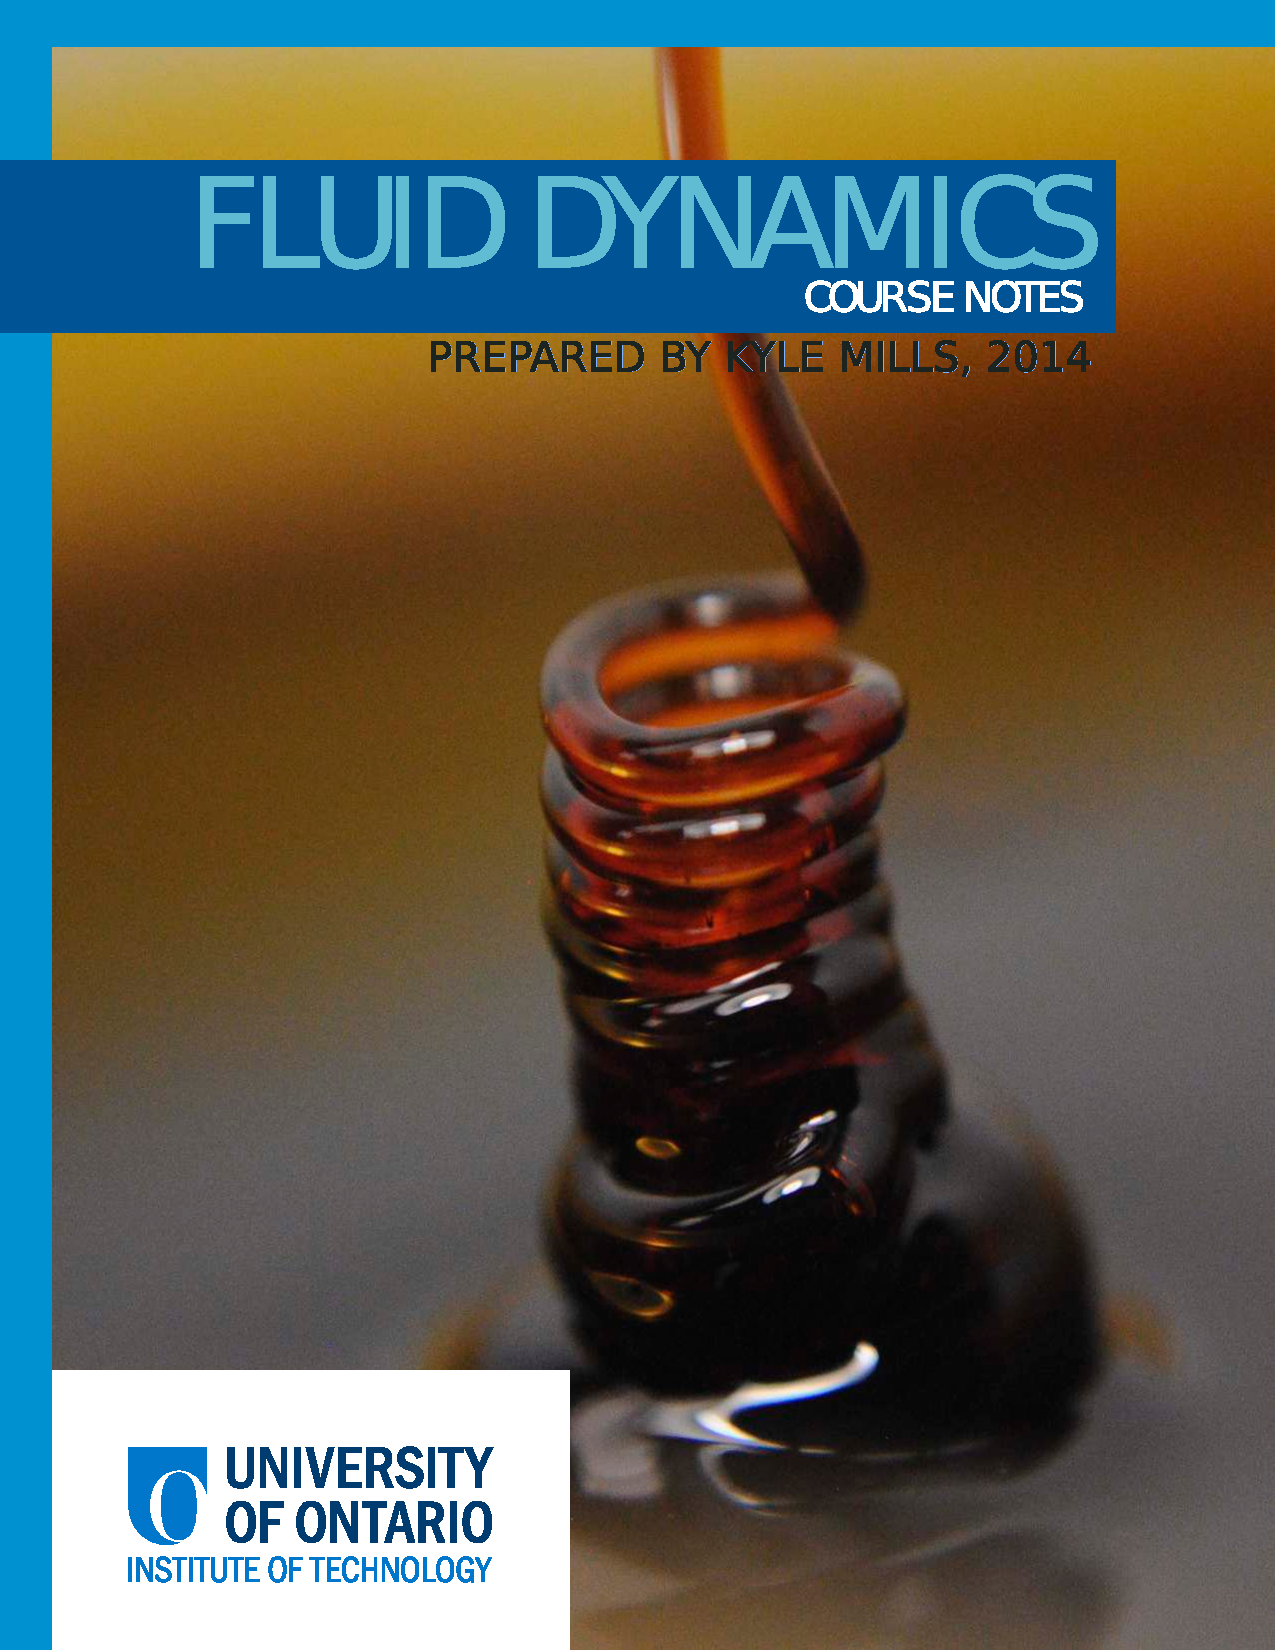
\includegraphics[width=\paperwidth,height=\paperheight]{extras/cover_compressed.pdf}}
%%%  }


%MY CUSTOM NU
\newcommand\xmysymbol{\raisebox{0.0ex}{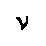
\includegraphics[height=1.1ex]{custom_symbols/nu.eps}}}
\renewcommand\nu{{\mathchoice{\xmysymbol}{\xmysymbol}{\hbox{\scriptsize\xmysymbol}}{\hbox{\tiny\xmysymbol}}}}



\begin{document}

\clearpage \mbox{}
\thispagestyle{empty}

\newpage

\newcounter{example}[chapter]
\newcounter{assignment}
\newcounter{problem}[chapter]
\newcounter{temporary}






\newpage
\tableofcontents
\newpage
\chapter{Introduction}
\section{What is a fluid?}
Before we begin our study of fluid dynamics we should look at what defines a substance as a fluid.  The simple answer is ``something that flows''.  While this may not seem satisfactory, it is true; almost anything that flows can be modeled by the equations and principles of fluid dynamics.  Examples are plentiful, the obvious choices being air and water, but even metals (when heated enough), electricity (electrons \textit{flow} through wires) and traffic flow can be modeled as fluids.


\section{Describing fluid flow}

The main goal of fluid dynamics is to determine the way in which a fluid moves.  In order to accomplish this, we need a function which describes the velocity of the fluid at every point in space and time:
\numeq{\vec u \equiv \vec u (\vec x, t)}{1velocitydefinition}
where $\vec x$ is a spatial vector, made up of three components. \Equation{1velocitydefinition} can also be written, perhaps more clearly as 
\numeq{\vec u \equiv \vec u (x,y,z,t) = [u,v,w].}{1velocityexplicit}
This function has three dimensions plus a time dependence, making it fairly complicated to model real fluids.  We'll begin by making two assumptions in order to simplify the theory:
\begin{enumerate}[i. ]
\item{$\vec u$ is not dependent on time (steady flow):\ \  $\partial \vec u / \partial t = 0$,}
\item{the flow is two-dimensional\footnote{This is not to say that every fluid flows as an infinitesimally thin sheet, but rather that there is symmetry such that we can neglect the $z$ component of $\vec u$ without a loss of information.}: \ \ $\vec u = \vec u (x,y,t)$}
\end{enumerate}
The combination of these assumptions gives rise to a simplified function 
\numeq{\vec u \equiv \vec u(x,y) = [u(x,y),\  v(x,y)]}{12dsteadyflow} modelling two-dimensional steady flow.



\section{Streamlines}
A streamline is defined as a curve that at time $t$ has the same direction as $\vec u (\vec x,t)$.  It represents an instantaneous snapshot of the fluid, representing the flow at one specific instant in time. The streamlines are parametrized by $s$, thus the slope of a streamline in the $x$ direction is given by $d x/d s$ and is proportional to the $x$-component of the velocity.  The same goes for the $y$ and $z$ components, giving
\numeq{\dd{x}{s} = ku \qquad\qquad \dd{y}{s} = kv \qquad\qquad \dd{z}{s}=kw. }{parametrizeddifferentials}
The proportionality constant $k$ is the same in each case, so 
\numeq{\frac{dx/ds}{u} = \frac{dy/ds}{v} = \frac{dz/ds}{w}.}{streamlineequation}
\Example{900626203739298376592938474629385}{
Compute the streamlines of
\unnumeq{\vec u = [x,\ \ x(x-1)(y+1)]}
}{
We know that $\vec u$ is of the general form $\vec u = [u,v,w]$, so in this case, $u=x$, $v=x(x-1)(y+1)$ and $w=0$.  \ \  \Equation{streamlineequation} reads as
\unnumeq{\frac{dx/ds}{x} = \frac{dy/ds}{x(x-1)(y+1)  }\qquad\Rightarrow\qquad dx = \frac{dy}{(x-1)(y+1) }.}
This differential equation is easy to solve using separation of variables. Integration of both sides yields
\unnumeq{\int{\!\!(x-1)\ dx} = \int{\!\!\!\frac{1}{y+1}}\ dy  \qquad\Rightarrow\qquad  \frac{1}{2}x^2 - x + C = \ln(y+1).}
Therefore the streamlines are given by
\unnumeq{y(x) = \exp\left[\frac{1}{2}x^2 - x + C\right] - 1.}
\Figure{fig/examplestreamlines.eps} shows the streamlines of 9 values of $C$. 
}
\insertfigure{fig/examplestreamlines.eps}{0.5}

\section{The total derivative and acceleration}
Let $f(x,y,z,t)$ be some quantity of interest.  It could be the a component of the velocity of the fluid, the density of the fluid or some other quantity.  If we're looking at one point in space $(x,y,z)$, then $\partial f / \partial t$ gives the rate of change of $f$ \textit{at that position}.  We don't want to be limited to one specific position; we'd rather ``move with the fluid'' and know how $f$ changes as we go along with the flow.  Rather than taking the partial derivative with respect to time, we should take the \textit{total derivative}.  The total derivative of $f$ is given by
\numeq{\frac{Df}{Dt} = \dd{}{t} \left[ f\left( x(t), y(t), z(t), t\right)\right]. }{totalderivative1}
Invoking the chain rule expands the total derivative to
\numeq{\frac{Df}{Dt} = \pp{f}{x}\pp{x}{t} + \pp{f}{y}\pp{y}{t} + \pp{f}{z}\pp{z}{t} + \pp{f}{t}.}{totalderivative2}
Looking back to \Equation{1velocityexplicit}, we can see that $\partial x / \partial t = u,\  \partial y / \partial t = v$ and $\partial z / \partial t = w$.  The total derivative is then
\numeq{\frac{Df}{Dt} = u\pp{f}{x} + v\pp{f}{y} + w\pp{f}{z} + \pp{f}{t}.}{totalderivative3}
It can be condensed to the form
\numeq{\frac{Df}{Dt} = \pp{f}{t} + \left(\vec u \cdot \grad \right)f.}{fullderivativeFinal}
It's important to note the order of operations; take the dot product of $\vec u$ with $\Nabla$ first and then operate on $f$.
In the case where $f=\vec u$, \Equation{fullderivativeFinal} can be viewed as the acceleration of the fluid, and is dependent on both space and time.

\Example{652983298267329843298732764329629209209347462}{A fluid is in uniform rotation in the $x,y$ plane with angular speed $\Omega$.  What is $\vec u$?  What is the acceleration?
}{
The linear velocity is related to the angular velocity through
\numeq{\vec u = \Omega \khat \cross \vec r}{linearangularvelocityequation}
Performing the cross product gives
\numeq{\vec u = [ -\Omega y\comma \Omega x\comma 0]}{ex2solution}
The flow is uniform (steady flow) so $\partial\vec u/\partial t = 0$, but the total derivative is
\begin{align*}
\frac{D \vec u}{Dt} &= \left(\vec u \cdot \vec\Nabla\right)\vec u \\
&= \left(u \pp{}{x} + v\pp{}{y} + w\pp{}{z}\right)\vec u \\
&= \left(-\Omega y \pp{\vec u}{x} + \Omega x\pp{\vec u}{y} \right)\vec u \\
&=-\Omega^2 y \jhat - \Omega^2 x \ihat \\
&=-\Omega ^ 2 \vec r
\end{align*}
where $\vec r$  is the position vector $\vec r = x\ihat + y\jhat$.
}

Returning for a moment to \Equation{fullderivativeFinal}, in any steady flow, the rate of change of $f$ is $(\vec u \cdot \Nabla)f$ for any fluid element.  If $(\vec u \cdot \Nabla)f = 0$, it means that $f$ is constant along a streamline.  It could be a \textit{different} constant along another streamline, but along any given streamline, $f$ is constant.  If ${Df}/{Dt} = 0$, $f$ is constant for the particular fluid element.  Again, it doesn't mean that other fluid elements will have the same value of $f$, but it does mean that for any particular fluid element, $f$ will not change.


\section{Viscosity}
As a fluid flows along a boundary, say in a pipe, it does not not slip along the surface of the pipe.  The fluid elements that are in direct contact with the boundary have zero velocity.  There exists a \textbf{boundary layer} where a velocity gradient is present.  Traversing the boundary layer, the flow speed increases rapidly and smoothly from zero to the normal flow speed $\vec u$.  Inside the boundary layer, the viscosity of the fluid cannot be neglected and the fluid follows \textbf{viscous theory}.

If a fluid is moving fast enough past an object, turbulence on the non-incident side of the object will exist.  The Reynolds Number, $R_e$ describes when turbulence will arise.  The Reynolds Number is defined as
\numeq{R_e\equiv \frac{uL}{\nu}}{ReynoldsNumber}
where $u$ is the flow speed, $\nu$ is the kinematic viscosity and $L$ is a length scale.\nopagebreak[6]  The Reynolds Number is a measure of when a fluid will become turbulent.\\




\Problem{Consider the two-dimensional flow given by
\unnumeq{\vec u = [\alpha x, -\alpha y ]}
where $\alpha$ is a positive constant. Is the flow \textit{incompressible}?  Sketch the streamlines of the flow.
Suppose a pollutant is introduced into the fluid and its concentration is given by 
\unnumeq{c(x,y,t) = \beta x^2 y e^{-\alpha t}} for $y>0$ and where $\beta$ is a constant. Does the pollutant concentration for any particular fluid element change with time?
}{
The flow is incompressible if $\vec\Nabla\cdot\vec u = 0$\ \  (\Equation{divergenceofvelocityequalszero}).
\begin{align*}
\vec\Nabla\cdot\vec u &= \pp{}{x}(u) + \pp{}{y}(v) \\
&= \pp{}{x}(\alpha x) + \pp{}{y}(-\alpha y) \\
& = \alpha - \alpha\\
&=0
\end{align*}
Therefore the flow is compressible. The streamlines can be computed by using \Equation{streamlineequation}.
\begin{align*}
\frac{dx/ds}{u} \quad&=\quad \frac{dy/ds}{v} \\
\int{\!\!\frac{dx}{\alpha x}} \quad&=\quad \int{\!\!\frac{dy}{-\alpha y}} \\
\frac{1}{\alpha}\ln\ x \quad&=\quad -\frac{1}{\alpha}\ln\ y + C \\
y(x) \quad&=\quad \frac{C}{x}\\
\end{align*}
Streamlines for $C=-4$ to $4$ are plotted in \Figure{fig/ass1/stagnation_streamlines.pdf}.  The total derivative (\Equation{fullderivativeFinal}) tells us whether the pollutant concentration for any particular fluid element changes with time.
\begin{align*}
\frac{Dc}{Dt} &= \pp{c}{t} + (\vec u \cdot \vec\Nabla ) c \\
  &= \beta x^2 y (-\alpha) e^{-\alpha t} + u \pp{c}{x} + v\pp{c}{y}\\
  &= \beta x^2 y (-\alpha) e^{-\alpha t} + \alpha x \pp{c}{x} -\alpha y \pp{c}{y}\\
  &= \beta x^2 y (-\alpha) e^{-\alpha t} + 2\beta x^2 y \alpha e^{-\alpha t} - \alpha\beta x^2 y e^{-\alpha t}\\
&= 0\\
\end{align*}
So the concentration of the pollutant in any fluid element does not change in time.
\insertfigure{fig/ass1/stagnation_streamlines.pdf}{0.8}
}



\Problem{Consider the \textit{unsteady} flow
\unnumeq{\vec u =[u_0, kt],} where $u_0$ and $k$ are constants.  Find the equation for the streamlines and show that they are straight lines at any particular point in time.  What happens as time goes on?  Show that the path a fluid particle follows is parabolic rather than a straight line.
}{
Once again we use \Equation{streamlineequation} to find the streamlines.
\unnumeq{\frac{dx/ds}{u} = \frac{dy/ds}{v} \qquad\Rightarrow\qquad \frac{dx}{u_0} = \frac{dy}{kt}}
Integration of both sides gives
\unnumeq{\frac{1}{u_0}x + C = \frac{1}{kt}y,}
so the streamlines are
\unnumeq{y(x) = \frac{kt}{u_0}x + C.}
At a particular point in time, $t$ can be considered constant, and $y$ varies linearly with $x$.  As time progresses, the slope of the streamline increases.  To find the actual path that the particle takes in the $i$ direction, we must integrate the $i$ component of velocity over time:
\unnumeq{x_i = \int{\!\!u_i dt.}}
So then the path of the particles is
\begin{align*}
\vec x &= \left[\textstyle  \int\!\! u_0 dt\comma\ \  \int\!\! ktdt \comma\ \  0  \right]\\
\vec x &= \left[u_0t+C\comma\  \ \frac{1}{2}kt^2 + D\comma\ \ K \right]\\
\end{align*}
where $C$, $D$ and $K$ are constants of integration.
}












\chapter{Ideal fluids}
\section{Properties of ideal fluids}
Now comes the time to begin looking at the physics of fluids.  We will first introduce the concept of an ideal fluid, a fluid which \textit{i)} is incompressible, \textit{ii)} is of constant density and \textit{iii)} exerts a force $p\vec n\ \delta S$ on a surface element $\vec n\  \delta S$.
\subsection{Incompressibility of ideal fluids}\label{section:Incompressibilityofidealfluids}
The incompressibility constraint can be easily thought of by considering a single fluid element, say a blob of dye.  If the fluid is incompressible, the blob is not permitted to change volume.  Mathematically, consider a fixed, closed surface $S$ within the fluid. Fluid can flow into and out of $S$, but we know the net volume cannot change, thus
\numeq{\int_{\mathcal S} \vec u \cdot \nhat \ dS=0}{fluxintout}
represents the rate of fluid flow across the surface in units of volume per time (here we took the speed of the fluid in length per time and integrated over the surface, multiplying by units of area). 
The divergence theorem states that
\numeq{\int_{\mathcal S} \vec u \cdot \nhat \  dS = \int_{\mathcal V} \vec\Nabla\cdot\vec u \  dV.}{divergencethm}
The only way this can be true and equal to zero is if 
\numeq{\vec\Nabla\cdot\vec u = 0.}{divergenceofvelocityequalszero}
\Equation{divergenceofvelocityequalszero} is known as the \textbf{incompressibility condition}.


\Problem{Consider the rate of mass flow through a fixed, closed surface $S$ drawn in the fluid. Following similar arguments made in Section \ref{section:Incompressibilityofidealfluids}, show that, even for compressible fluids, conservation of mass implies that
\numeq{\pp{\rho}{t} + \div(\rho\vec u)=0.}{conservationofMass}
}{
Similarly to how we obtained \Equation{fluxintout}, we can multiply the speed of the fluid by the density $\rho$ and integrate over the entire surface.  
\unnumeq{\int_{\mathcal S}\rho\vec u \cdot \nhat\ dS}
This gives us the mass flow rate, in kg/s.  If there is a net mass ``flux'', then the density of the enclosed fluid must change (if we're packing more mass into the same volume, the density must be changing). The mass rate will be equal to the rate of change of density integrated over the entire volume. This means that 
\unnumeq{\int_{\mathcal S}\rho\vec u \cdot \nhat\ dS = -\int_{\mathcal V} \pp{\rho}{t}\ dV}
(the negative arises since $\nhat$ points out of the surface.  If the density is increasing, the mass inside is increasing and the net flow is against $\nhat$).
Applying the divergence theorem to the first term changes it from a surface to a volume integral
\unnumeq{\int_{\mathcal V}\div (\rho \vec u)\ dV = -\int_{\mathcal V} \pp{\rho}{t}\ dV} in which both integration volumes are identical allowing us to drop the integrals, leaving only
\unnumeq{\div (\rho \vec u) =  -\pp{\rho}{t}}
or
\unnumeq{\pp{\rho}{t} + \div (\rho \vec u) =0.}

}



\subsection{Density of ideal fluids}
An ideal fluid is one that has constant density $\rho$ (mass per unit volume).  Every fluid element has the same density at all time, that is
\numeq{\dd{\rho}{t} = 0.}{constantdensityintime}

\subsection{Forces in an ideal fluid}
The force exerted by the surrounding fluid across any surface element $dS$ is given by $p\nhat\ dS$, where $p\equiv p(x,y,z,t)$ represents pressure.  There are no tangential forces which act on the surface. Mathematically, 
\numeq{d\vec F = -p\nhat dS}{infinitesimalforce}
so using the identity $\oint_{\mathcal S} \vec \varphi \nhat dS = \int_{\mathcal V}\Nabla\vec \varphi dV$  (for an arbitrary vector $\vec a$),  
\numeq{\vec F = \int_{\mathcal V}\Nabla p\   dV}{exertedforces}


\section{Euler's equations of motion}
\subsection{Gravity on an ideal fluid}
\Equation{exertedforces} gives us the force exerted on an element of the fluid by the surrounding fluid, but any fluid in a gravitational field will also experience a downward gravitational force which cannot be neglected.   The total force is then
\numeq{\vec F = \int_{\mathcal V} \Nabla p dV + m\vec g}{netforce1}
but the total mass $m$ can be represented by $\int_{\mathcal{V}}\rho d V$ so
\numeq{\vec F = \int_{\mathcal V} \left( -\Nabla p + \rho \vec g\right) dV.}{eulernetforce}
Dividing everything by $m=\rho V$ and recalling $\int_{\mathcal V} dV = V $ and $ \vec F/m  = D\vec u /Dt$ gives 
\numeq{\frac{D \vec u }{Dt} = -\frac{1}{\rho} \Nabla  p  + \vec g.}{EulersEquationPrimaryForm}
This, along with the incompressibility condition of \Equation{divergenceofvelocityequalszero} constitutes Euler's Equations.
We can represent the vector $g$ as a the gradient of the scalar potential $\chi=gz$, changing \Equation{EulersEquationPrimaryForm} into 
\numeq{\frac{D\vec u }{ Dt} = -\frac{1}{\rho}\Nabla  p  - \Nabla \chi.}{eulerwithgravitygradient}
Equating this with the left-hand side of the total derivative (\Equation{totalderivative1}) gives
\numeq{\pp{\vec u }{t} + \left( \vec u \cdot \Nabla \right)\vec u = -\frac{1}{\rho}\Nabla p  - \Nabla\chi}{962394566982764309743509245}
Using the identity $(\vec u \cdot \Nabla)\vec u = (\Nabla\cross\vec u )\cross\vec u +\frac{1}{2} \Nabla(\vec u \cdot \vec u)$
we can rewrite \Equation{962394566982764309743509245} as
\numeq{\pp{\vec u}{t} + (\Nabla \cross \vec u ) \cross \vec u + \frac{1}{2}\Nabla(\vec u ^2) = -\frac{1}{\rho}\Nabla  p  - \Nabla \chi}{527039847520}
and since the gradient is a linear operator, we can move all of them to the right hand side and obtain
\numeq{\pp{\vec u}{t} + (\Nabla \cross \vec u ) \cross \vec u  = -\Nabla \left(  \frac{1}{2}(\vec u ^2)+\frac{1}{\rho} p  +  \chi \right).}{5270398475204}
We'll define the three terms in the left parenthesis as 
\numeq{H\equiv  \frac{1}{2}(\vec u ^2)+\frac{1}{\rho} p  +  \chi}{bernoulliHdefinition}
and then \Equation{5270398475204} becomes
\numeq{\pp{\vec u}{t} + (\Nabla \cross \vec u ) \cross \vec u  = -\Nabla H.}{0928370923486530497658}

\subsection{Bernoulli streamline equation}

Why did we bother to obtain \Equation{0928370923486530497658}?  Firstly, if the flow is steady ($\partial \vec u / \partial t = 0$), then it becomes
\numeq{(\Nabla \cross \vec u ) \cross \vec u  = -\Nabla H.}{987423094820394820398475}
of which we can take the dot product with $\vec u$ and obtain
\numeq{\vec u \dot \left( (\Nabla \cross \vec u ) \cross \vec u \right)=(\vec u \dot \Nabla ) H.}{129876542309457230948720394}
The left hand side evaluates to zero\footnote{
	How?  Well, $\curl{\vec u}$ will yield a vector perpendicular to \vec u, which when crossed with \vec u will 		also inevitably be perpendicular to \vec u.  The dot product of two perpendicular vectors is zero.} 
which allows us to conclude that
\numeq{ (\vec u \dot \Nabla )H = 0,}{BernoullisStreamlineEquation}
meaning that if an ideal fluid is in steady flow, then $H$ is constant along a streamline.


\section{Irrotational Flow}
Irrotational flow is flow such that 
\numeq{\gvec \omega \equiv \Nabla\cross\vec u = 0}{irrotationalflowdefinition}
where \gvec\omega is called the \textit{vorticity}.
For steady, irrotational flow, the Euler equation reduces to
\numeq{\Nabla H = 0}{dsfsgskjsadhflkusa}
which means that $H$ is constant throughout the fluid.


\Example{93698256924396109437230928743206}{What is the vorticity of a two dimensional fluid?}{A two-dimensional fluid is given by
\unnumeq{\vec u = [u\comma v\comma 0] }
where $u = u(x,y,t)$ and $v = v(x,y,t)$.
The vorticity is then
\unnumeq{ \gvec \omega  = \Nabla\cross\vec u = \curlArray{x}{y}{z}{u}{v}{0} = \left(0-\pp{v}{z}\right)\ihat - \left(0-\pp{u}{z}\right)\jhat + \left(\pp{v}{x} - \pp{u}{y}\right)\khat}
Since $u$ and $v$ are not dependent on $z$,\ \ $\partial u/\partial z = \partial v / \partial z = 0$ and
\unnumeq{\gvec\omega = \left ( \pp{v}{x} - \pp{u}{y}\right) \khat}
We'll be dealing with two-dimensional flow so much that we'll define this result as $\omega$ (scalar) such that
\numeq{\gvec\omega \equiv \left( \dd{v}{x} - \dd{u}{y}\right) \khat = \omega \khat}{skdjhfakdshfaksjdf}

}


\Example{ExVorticityNotRotatingFluid}{   Calculate the vorticity $\omega$ for the flow
\unnumeq{\vec u = [\beta y ,0,0].}
}
{From the vector plot, we can see that the fluid is clearly not rotating, but let's calculate the vorticity anyway:
\unnumeq{\gvec\omega=\curl{\vec u} = \curlArray{x}{y}{z}{\beta y}{0}{0} = 0\ihat - \left(\pp{\beta y}{z} - 0\right)\jhat + \left(0 - \pp{\beta y }{y}\right)\khat = -\beta \khat}
There is a constant vorticity even though the flow does not rotate.  This demonstrates a very significant property of vorticity:  not all fluids that have vorticity rotate.
}

\Example{ExVorticityPolarCoordinates}{ Consider the flow
\unnumeq{\vec u  = \frac{K}{r}\gvec{\hat\theta }}
given in cylindrical coordinates ($\gvec{\hat\theta} = -\sin\theta\ihat + \cos\theta\jhat$).  Find the vorticity. What happens at the origin ($r=0$)?

}{\unnumeq{  \gvec\omega = \curl{\vec u} = \frac{1}{r}\cylindricalcurlArray{u_r}{ru_\theta}{u_z} = \frac{1}{r}\cylindricalcurlArray{0}{K}{0} = 0}
When $r=0$, $\omega=0/0$;  there is a singularity at the origin.
}
After investigating vorticity in the previous three examples we are left wondering exactly what it is.  Example \thechapter.\ref{ExVorticityNotRotatingFluid} showed that a non-rotating fluid had constant non-zero vorticity, while Example \thechapter.\ref{ExVorticityPolarCoordinates} showed that a specific fluid which is clearly rotating does not have vorticity.  It turns out that vorticity is a measure of the \textit{local rotation}, not the global rotation of the fluid.

\Example{ExFinalIdealFluidExample}{Consider an ideal fluid rotating under gravity with constant angular velocity $ \Omega$ (say, water rotating in a water bottle).  What is the fluid velocity \vec u in Cartesian coordinates?  What is the shape of the free surface (the boundary between water and air)?}
{
$\gvec \Omega = (0,\ 0,\ \Omega) = \Omega\khat$ is a vector that points along the $z$-axis.  By \Equation{linearangularvelocityequation}, the velocity is  then
\unnumeq{\vec u =\gvec \Omega \cross \vec r = \crossArray{\ihat}{\jhat}{\khat}{x}{y}{z}{0}{0}{\Omega} = \Omega y \ihat - \Omega x\jhat = (-\Omega y, \Omega x)}
The surface of the water is distinguished by being at atmospheric pressure. Everywhere along the surface, $p=p_0$.
Equating Euler's equation (\Equation{EulersEquationPrimaryForm}) with the total derivative (\Equation{totalderivative1}) gives us
\unnumeq{\frac{D\vec u}{Dt} = \pp{\vec u}{t} + \left(\vec u \dot \Nabla\right)\vec u = -\frac{1}{\rho}\Nabla  p  + \vec g.}
This is really three equations; one for $x$, one for $y$ and one for $z$.  By expanding the dot product and gradient for each coordinate, we can obtain
\begin{align*}
x&:\quad \pp{u}{t} + u\pp{u}{x} + v\pp{u}{y} + w\pp{u}{z} = -\frac{1}{\rho}\pp{ p}{x}   \\
y&:\quad \pp{v}{t} + u\pp{v}{x} + v\pp{v}{y} + w\pp{v}{z} = -\frac{1}{\rho}\pp{ p}{y}   \\
z&:\quad \pp{w}{t} + u\pp{w}{x} + v\pp{w}{y} + w\pp{w}{z} = -\frac{1}{\rho}\pp{ p}{z} -  g   
\end{align*}
Most of these terms are zero; they reduce to
\begin{align*}
x&:\quad \pp{p}{x} = \rho \left(v \pp{u}{y}\right) = -\rho\Omega y (-\Omega) = \rho\Omega^2x   \\
y&:\quad \pp{p}{y} = \rho \left(u \pp{v}{x}\right) = \rho\Omega x (\Omega) = \rho\Omega^2y   \\
z&:\quad \pp{p}{z} = -\rho g
\end{align*}
The only quantity that we don't know is the pressure, the derivative of which is
\unnumeq{dp = \pp{p}{x}dx + \pp{p}{y}dy + \pp{p}{z}dz.}
By inserting the partial derivatives we obtained for each component and integrating we get
\begin{align*}
\int\!\! dp &= \int\!\!\rho\Omega^2 x\  dx + \int\!\!\rho\Omega^2 y\ dy  -  \int\!\!\rho g\ dz \\
p - p_0 &= \frac{1}{2}\rho \Omega^2 x^2 + \frac{1}{2}\rho \Omega^2 y^2 - \rho g z \\
& = \frac{1}{2}\rho \Omega^2 (x^2 + y^2) - \rho gz
\end{align*}
We want the free surface which we know is at constant pressure. The surface will be given by the $z$-coordinate at each $(x,y)$ point, thus setting $(p-p_0)$ constant and solving for $z$ gives
\unnumeq{ z = \Omega^2(x^2 + y^2) - (p - p_0)}
as the surface of constant pressure, and the surface of the water.  \Figure{fig/ch2/paraboloid_vortex.pdf} shows  the surface and we can see that it looks much like the ``vortex'' that appears in a water bottle.\nopagebreak
\insertfigure{fig/ch2/paraboloid_vortex.pdf}{1.1}

}





\startAssignment
\Problem{Calculate the divergence and curl for each of the following vector functions:
\begin{align*}
\mathrm{(i)}\quad  &   \vec u_{1} = [x^2, 3xz^2, -2xz] \\
\mathrm{(ii)}\quad  &  \vec u_{2} = [xy, 2yz, 3zx] \\
\mathrm{(iii)}\quad  & \vec u_{3} = [y^2, 2xy + z^2, 2yz] \\
\end{align*} Prove that the curl of a gradient is always zero, and prove that the divergence of a curl is always zero.
}{
First, let's review what the divergence and curl are for any three-dimensional vector function $\vec F$ where
\unnumeq{\vec F = [u, v, w] = u\ihat + v\jhat + w\khat.}
\numeq{\mathrm{div}\ \vec F = \div\vec F = \pp{u}{x} + \pp{v}{y} + \pp{w}{z}}{divergenceOfvectorfunction}
\numeq{\mathrm{curl}\ \vec F = \curl\vec F = \curlArray{x}{y}{z}{u}{v}{w}}{curlOfvectorfunction}
$\curl \vec F$ can be expanded and written more explicitly as
\numeq{\curl{\vec F} = \left(\pp{w}{y} - \pp{v}{z}\right)\ihat + \left( \pp{u}{z}-\pp{w}{x}\right)\jhat + \left(\pp{v}{x} - \pp{u}{y}\right)\khat}{expandedcurlofarbitraryvector}
The divergence of a vector is a scalar.  The curl of a vector is a vector. So
\begin{align*}
&\div\vec u_1 = \pp{}{x}\left(x^2\right) + \pp{}{y}\left(3xz^2\right) + \pp{}{z}\left(-2xz\right) = 2x +0-2x = 0 \\
&\curl \vec u_1 = \triplecomponentvector{0 - 6xz}{0-(-2z)}{3z^2 - 0} = -6xz\ihat + 2z\jhat + 3z^2\khat  \\
&\div\vec u_2 = \pp{}{x}\left(xy\right) + \pp{}{y}\left(2yz\right) + \pp{}{z}\left(3zx\right) = y + 2z + 3x\\
&\curl\vec u_2 = \triplecomponentvector{0-2y}{0 - 3z}{0-x} = -2y\ihat - 3z\jhat -x\khat \\
&\div\vec u_3 = \pp{}{x}\left(y^2\right) + \pp{}{y}\left(2xy + z^2\right) + \pp{}{z}\left(2yz\right) = 0 + 2x + 2y = 2(x + y) \\
&\curl\vec u_3 = \triplecomponentvector{2z - 2z}{0 - 0}{2y - 2y} = 0\ihat + 0\jhat + 0\khat = \vec 0 \\  
\end{align*}
To prove that the curl of a gradient is always zero, let $f$ be a scalar function.  The gradient of $f$ is 
\numeq{\grad f = \pp{f}{x}\ihat + \pp{f}{y}\jhat + \pp{f}{z}\khat }{gradientOfArbitraryFunction}
Then
\renewcommand{\arraystretch}{1.5} %larger space in matrix
\begin{align*}\curl (\grad f) &= \curlArray{x}{y}{z}{\pp{f}{x}}{\pp{f}{y}}{\pp{f}{z}} \\
&= 
\left(\pp{^2f}{y\partial z} - \pp{^2f}{z\partial y}\right)\ihat + 
\left(\pp{^2f}{z\partial x} - \pp{^2f}{x\partial z}\right)\jhat + 
\left(\pp{^2f}{x\partial y} - \pp{^2f}{y\partial x}\right)\khat
\end{align*}
and since order of differentiation doesn't matter, as long as $f$ is twice differentiable, all of the terms cancel and 
\numeq{\curl (\grad f) = \vec 0.}{curlofagradientiszero}
To prove that the divergence of a curl is always zero, I'll take the expanded form of the curl (\Equation{expandedcurlofarbitraryvector}) and apply the divergence operator (\Equation{divergenceOfvectorfunction}):
\unnumeq{\div (\curl \vec F)  =  \pp{}{x}\left(\pp{w}{y} - \pp{v}{z}\right) + \pp{}{y}\left( \pp{u}{z}-\pp{w}{x}\right) + \pp{}{z}\left(\pp{v}{x} - \pp{u}{y}\right)}
Differentiation is a linear operator; we can expand the parenthesis:
\unnumeq{\div (\curl \vec F)  = \dpp{w}{x}{y} - \dpp{v}{x}{z} + \dpp{u}{y}{z} - \dpp{w}{y}{x} + \dpp{v}{z}{x} - \dpp{u}{z}{y}}
Again, as long as each component of $\vec F$ is twice-differentiable, order of differentiation doesn't matter and all of the terms cancel.  Therefore
\numeq{\div (\curl \vec F)  =0}{divergenceofacurliszero}
\renewcommand{\arraystretch}{1.0}
}



\Problem{Consider a fluid at rest.  Show that the free surface must be a horizontal plane.  How does the pressure change with depth within the fluid? (Hint: derive $p=p(d)$ where $d$ is the distance below the free surface)
}{
The fluid is at rest so Euler's equation is given by
\unnumeq{\frac{D\vec u }{Dt} = -\frac{1}{\rho}\grad p + \vec g = 0}
since $D\vec u / Dt = 0$.  Rearranging this gives
\unnumeq{\grad p = -\rho \vec g.}
Since $\grad p$ and $\vec g$ are both three-dimensional vectors, we have really obtained three equations. 
\begin{align*}
x:&\qquad \pp{p}{x} = -\rho g_x = 0 \\
y:&\qquad \pp{p}{y} = -\rho g_y = 0 \\
z:&\qquad \pp{p}{z} = -\rho g_z = -\rho g
\end{align*}
The $\partial p / \partial x = \partial p /\partial y = 0$ since gravity only acts in the $z$ direction.  It's for this same reason that $\partial p / \partial z$ survives as $-\rho g$.
The total derivative of pressure can be taken:
\unnumeq{dp = \pp{p}{x}dx + \pp{p}{y}dy + \pp{p}{z} dz}
This reduces to 
\unnumeq{dp = -\rho g dz}
since (from above) the first two partial derivatives are zero. Integrating both sides yields
\unnumeq{p = -\rho g z + p_0}
So the pressure \textit{difference} between the surface of the fluid and a point $-z$ below the fluid surface is
\unnumeq{p = p_0 - \rho g z.}
Additionally, we can find the surface of constant pressure by rearranging for $z$,
\unnumeq{z = - (p-p_0)/\rho g} 
Thus the surface of the fluid is a horizontal plane (all quantities on the right are constants).
}



\Problem{Consider the Rankine vortex defined by the flow
\unnumeq{u_\theta = 
\left\{\begin{array}{ll}
\Omega r & r<a \\
\frac{\Omega a^2}{r} & r>a \\ 
\end{array}
\right.}
Find the pressure both inside the radius $a$ and outside, and show that the difference in pressure between $r=0$ and $r=\infty$ is 
\unnumeq{\Delta p = \rho\Omega^2a^2.}
}{First, let's begin by examining the case when $r>a$.  For $r>a$
\unnumeq{ \vec u = [ u_r, u_\theta, u_z ] = [0,\  \Omega a^2/r,\  0].}
Now, we could use Euler's equations as we did in Example \thechapter.\ref{ExFinalIdealFluidExample}, but that is a lot of work.  We'll use a different approach; we'll calculate the vorticity of the fluid:
\unnumeq{\curl \vec u = \frac{1}{r}\cylindricalcurlArray{0}{\Omega a^2}{0} = 0}
Great!  The vorticity is zero, which means we can use \Equation{987423094820394820398475} to easily obtain the pressure. 
\unnumeq{\left(\curl\vec u\right)\cross\vec u = -\grad H}
Since $\curl\vec u = 0$,
\unnumeq{-\grad H = 0.}
We defined $H$ as 
\unnumeq{H = \frac{1}{2}\vec u^2 + \frac{1}{\rho}p + gz}
so this means that
\unnumeq{0 = -\grad \left(  \frac{1}{2}\vec u^2 + \frac{1}{\rho}p + gz    \right).} 
We can simplify this to
\unnumeq{0 = -\grad \left(  \frac{\rho \Omega ^ 2 a^4 }{2r^2} + p + \rho gz    \right)}
since $\vec u ^2 = \vec u\dot\vec u = (u_r^2 + u_\theta^2 + u_z^2) = u_\theta^2=\Omega^2 a^4 / r^2$. The gradient is a linear operator so we can move $-\grad p$ to the left and obtain
\unnumeq{\grad p = -\grad \left(  \frac{\rho \Omega ^ 2 a^4 }{2r^2} +  \rho gz    \right).} 
Integrating both sides (the ``inverse'' of the gradient) gives
\unnumeq{p(r,z) = -\frac{\rho\Omega^2a^4}{2r^2} - \rho g z + p_{0_1}}
where $p_0$ is the pressure at $r=\infty$ and $z=0$.
So we've found the pressure when $r>a$, but what about $r<a$?  If we follow the same procedure we find that
\unnumeq{\curl\vec u = \frac{1}{r}\cylindricalcurlArray{0}{\Omega r^2}{0} = \frac{1}{r}(2\Omega r \zhat) = 2\Omega\zhat.}
This time, the vorticity is nonzero!  In order to use \mbox{$\left(\curl\vec u\right)\cross\vec u = -\grad H$} we must now find the cross product on the left.  We know $\curl\vec u=(0,\ 0,\ 2\Omega)$ so 
\unnumeq{ \left(\curl\vec u\right)\cross\vec u = \frac{1}{r}\crossArray{\rhat}{\thetahat}{\zhat}{0}{0}{2\Omega}{0}{\Omega r^2}{0} = -2\Omega^2 r \rhat}
and we know that this is equal to $-\grad H$.  We can write this out in full as
\unnumeq{ -2\Omega^2 r\rhat = -\grad\left(\frac{\Omega^2 r^2}{2} + \frac{p}{\rho} + gz\right)}
since this time $\vec u ^ 2 = \Omega^2r^2$. On the left hand side we have only an $\rhat$ contribution, thus the gradient on the right must yield only $\rhat$ components; $\lpp{H}{\theta} = \lpp{H}{z} = 0$. So working  implicitly in the $\rhat$ direction, the gradient can be rewritten as \lpp{}{r} giving
\unnumeq{2\Omega^2 r = \pp{}{r} \left(\frac{\Omega^2r^2}{2} + \frac{p}{\rho} + gz\right)}
which can be integrated with respect to $r$
\unnumeq{\int\! 2\Omega^2 r\ dr = \frac{\Omega^2r^2}{2} + \frac{p}{\rho} + gz}
to give
\unnumeq{\Omega^2 r^2 = \frac{\Omega^2r^2}{2} + \frac{p}{\rho} + gz.}
Solving for the pressure gives
\unnumeq{p(r,z) = \frac{\rho \Omega^2r^2}{2} - \rho g z + p_{0_2}.}
Now that we know the pressure of the fluid at any radius (whether it be larger than $a$ or not), we can find the difference between the pressure at the centre of the fluid ($r=0$) and $r=\infty$ by subtraction.
\unnumeq{\Delta p =  p(\infty, z) - p(0, z) = \left(-\frac{\rho\Omega^2a^4}{2r^2} - \rho g z + p_{0_1}\right) - \left(\frac{\rho \Omega^2r^2}{2} - \rho g z + p_{0_2}\right)}
When we plug in $r=\infty$ into the first parentheses, the first term disappears.  Similarly, when we plug in $r=0$ into the second parentheses, the first term also vanishes.  We're left with
\unnumeq{\Delta p = -\rho g z + \rho g z + p_{0_1} - p_{0_2} = p_{0_1} - p_{0_2}.}
In order to find this quantity, we apply the boundary condition; $p$ must be continuous at $r=a$, such that
\begin{align*}
\left. -\frac{\rho\Omega^2a^4}{2r^2}\right|_{r=a} - \rho g z + p_{0_1} &= \left.\frac{\rho \Omega^2r^2}{2}\right|_{r=a} - \rho g z + p_{0_2} \\[1em]
-\frac{1}{2}\rho\Omega^2a^2 + p_{0_1} &= \frac{1}{2}\rho \Omega^2a^2 + p_{0_2} \\[1em]
 p_{0_1} - p_{0_2} &= \frac{1}{2}\rho \Omega^2a^2 - (-\frac{1}{2}\rho\Omega^2a^2) \\
 p_{0_1} - p_{0_2} &= \rho \Omega^2a^2
\end{align*}
Therefore, the difference in pressure between $r=0$ and $r=\infty$ is $\Delta p =  \rho \Omega^2a^2$.
}


\stopAssignment

















\chapter{Classical Aerofoil Theory}\label{chapter:classicalaerofoiltheory}

\section{A Brief Introduction to Complex Numbers}
Later in this chapter we will use complex numbers quite extensively.  We'll quickly go over what complex numbers are and the different operations that will be useful.  A complex number $z$ is a number that can be expressed in the form $z=x+iy$, where $x$ and $y$ are real numbers and $i$ is the imaginary unit (ie: $i = \sqrt{-1}$).  $\Re{z} = x$ is called the \textit{real part of $z$}, while $\Im{z} = y$ is called the \textit{imaginary part of $z$}.  While real numbers can be represented by a point on a number line, complex numbers are represented by a point on the two-dimensional \textit{complex plane}, with the real part of $z$ plotted on the horizontal axis and the imaginary part of $z$ plotted on the vertical axis.
\insertfigure{fig/ch3/Complex_number_illustration.eps}{0.55}
It's evident from \Figure{fig/ch3/Complex_number_illustration.eps} that $x=r\cos\theta$ and $y = ir\sin\theta$ so Euler's formula allows us to write complex numbers also in radial form as
\unnumeq{z = x + iy = r(\cos\theta + i\sin\theta) = r\e{i\theta}}
where $r=\abs{z} = \sqrt{x^2 + y^2}$ is called the \textit{modulus} of $z$ and 
\unnumeq{\theta = \mathrm{Arg}(z) =  \arctan\left(\frac{y}{x}\right) = \arctan\left(\frac{\Im{z}}{\Re{z}}\right)}
 is called the argument of $z$.   The complex \textit{conjugate} of a complex number is given by 
\unnumeq{z\star = x - iy}
and is found explicitly by replacing every $i$ in a complex number with $-i$.  The complex conjugate corresponds with a reflection of the complex number over the real axis, thus the conjugate of the conjugate is the original complex number (ie: $(z\star)\star = z$).

\subsection{Algebra of complex numbers}
In many cases, complex numbers can be thought of as ``vectors'' with the imaginary part corresponding to the vertical component and the horizontal component corresponding to the real part.  Just like with vectors, the addition of two complex numbers is the addition of the real and imaginary parts separately.  That is, if $z_1 = x_1+iy_1$ and $z_2 = x_2+iy_2$, 
\begin{align*}
z_1 + z_2 &= (x_1+iy_1) + (x_2+iy_2) = (x_1 + x_2) + i(y_1 + y_2) \ \ \mathrm{and} \\
z_1 - z_2 &= (x_1+iy_1) - (x_2+iy_2) = (x_1 - x_2) + i(y_1 - y_2).
\end{align*}

Multiplication is the same as with purely real numbers, but when we multiply two complex numbers, we must take care to recognize that $i^2  = -1$, resulting in the product of two imaginary terms being real:
\unnumeq{z_1z_2 = (x_1+iy_1)(x_2+iy_2) = (x_1x_2 - y_1y_2) + i(x_1y_2 + x_2y_1).}

When two complex numbers must be divided, it's usually best to first obtain a common denominator by multiplying the numerator and denominator by the complex conjugate:
\unnumeq{\frac{z_1}{z_2} = \frac{x_1 + iy_1}{x_2 + iy_2} = \frac{(x_1 + iy_1)(x_2 - iy_2)}{(x_2 + iy_2)(x_2 - iy_2)} = \frac{(x_1x_2 - y_1y_2) + i(-x_1y_2 + x_2y_1)}{x_2^2 + y_2^2}.}
Notice that the denominator is now real, giving
\unnumeq{\frac{z_1}{z_2} = \left(\frac{x_1x_2 - y_1y_2 }{x_2^2 + y_2^2}\right) + i\left(\frac{x_2y_1 - x_1y_2  }{x_2^2 + y_2^2}\right).}




\subsection{Complex functions}
Just as $z$ is a complex number, made up of a real and imaginary parts, a complex \textit{function} is a function with both real and imaginary parts.  A complex function $f$ is given by
\unnumeq{f(z) = f(x + iy) = u(x,y) + iv(x,y)}
where $u$ and $v$ are real-valued functions of real variables $x$ and $y$.

\Example{complexexample1}{Write the function $f(z) = |z|^2z\star + \Im{z}$ in the form $f(x+iy) = u + iv$, identifying $u$ and $v$ explicitly.
}{
First, we'll replace every instance of $z$ with $x+iy$ since $u$ and $v$ are functions of $x$ and $y$, not $z$.
\unnumeq{f(z) = |z|^2z\star + \Im{z} =|x+iy|^2(x+iy)\star + \Im{x+iy}.}
We'll look at the various parts separately:
\begin{align*}
&|z|^2 = |x+iy|^2 = \left(\sqrt {x^2 + y^2}\right)^2 = x^2 + y^2.\\
&z\star = (x+iy)\star = x-iy\\
&\Im{z} = \Im{x + iy} = y
\end{align*}

Therefore,
\begin{align*}
f(z) = f(x + iy) &= (x^2 + y^2)(x-iy) + y \\
&=x(x^2 + y^2) + y - iy(x^2 + y^2) \\
&=\left(x^3 + xy^2 + y\right) - i\left(x^2y + y^3\right) \\
&=u + iv
\end{align*}
Therefore, $u = u(x,y) = x^3 + xy^2 + y$ and $ v = v(x,y) = x^2y + y^3$.
}

Sometimes it's much easier, or more logical to consider complex functions in polar form, that is, as functions of $r$ and $\theta$ instead of $x$ and $y$.  Equivalently, 
\unnumeq{f(z) = f(r\e{i\theta}) = u(r,\theta) + iv(r,\theta)}
where $u(r, \theta)$ and $v(r, \theta)$ are real-valued functions of $r$ and $\theta$.  For example, it would be tedious to find the real part of the complex-valued function $f(z) = z^8$, but in polar coordinates, the process is trivial:


\Example{complexfunctionexample2}{Write the complex function $f(z) = z^8$ in the form $f(z) = u+iv$, and identify $u$ and $v$ explicitly.
}{As discussed, it would be tedious to expand $f(z) = (x + iy)^8$ in Cartesian coordinates, so let's use polar coordinates instead.  We'll write $z$ in polar form as $z = r\e{i\theta}$, meaning
\unnumeq{f(z) = \left(r\e{i\theta}\right)^8 = r^8\e{i8\theta}}
so using Euler's formula, this becomes
\unnumeq{f(z) = r^8\left(\cos 8\theta + i\sin 8\theta\right) = \left(r^8\cos8\theta\right) + i\left(r^8\sin8\theta\right).  }
Therefore $u(r, \theta) = r^8\cos8\theta$ and $v(r, \theta) = r^8\sin8\theta$.

}










We'll use the concept of a complex function when we define the complex potential later in this chapter.  It will be important to understand how to separate the real and imaginary parts of complex numbers and complex functions as we'll find that the real parts and imaginary parts are meaningful individually.

\section{Potential Theory}
Up until now we've described fluid flow in terms of of various vector quantities (forces, velocities), but vectors are difficult to deal with (or at least more difficult than necessary), so we'll define some additional quantities, potentials, that allow us to describe more complicated flow in an simple manner.  These potentials are scalar quantities, and thus much easier to work with than vector quantities.
\subsection{The Velocity Potential, $\phi$}
Suppose we have a flow that is irrotational, that is $\curl\vec u = 0$.  Our goal is to eliminate the vectors, so how can we simplify this?  Well, we know that the curl of a gradient is zero, so this means that \vec u must be equivalent to the gradient of some scalar function.  We'll call this scalar function $\phi = \phi(x,y)$ and define it as
\numeq{\vec u \equiv \grad \phi,}{scalarfunctionu}
naming it the \textbf{velocity potential}.  A gradient is a three-dimensional derivative, so the inverse function is a line integral, giving
\numeq{\phi = \int\!\! \vec u \dot d\vec x}{inversescalarfunctionphi}
(remember \vec u and \vec x are vector functions, so this is really the sum of three integrals).  If the fluid occupies a simply connected region,\footnote{a simply connected region is one in which \textit{any} closed path lying in the region can be contracted in on itself until the path becomes a point:  a sphere is simply connected, but a donut is not.}  then $\phi$ is single valued.  If the fluid occupies a non-simply connected region, then $\phi$ will be multi-valued.
Now we could go back and write all of Euler's equations in terms of $\phi$, but let's instead develop a different way of attacking problems now that we have this new representation.
\Example{92305965093765j203946520394765j}{Find the velocity potential of the flow
\unnumeq{\vec u = (U\comma 0\comma 0)}
}{
\Equation{inversescalarfunctionphi} gives $\phi$ simply as
\unnumeq{\phi = \int \vec u \dot d\vec x = \int Udx = Ux + C}
}

\Example{0928747jd2034jd203984h50239j}{We'll take this one step further, our standard two dimensional flow.  Find the velocity potential of
\unnumeq{\vec u = (-\alpha x\comma -\alpha y\comma 0).}
}
{
Again \Equation{inversescalarfunctionphi} gives us $\phi$, but this time, we have both horizontal and vertical components, so
\unnumeq{\phi = \int\!\!\vec u\dot d\vec x = \int \!\! udx + \int\!\! vdy =  -\frac{1}{2}\alpha x^2 - \frac{1}{2}\alpha y^2 + C} 
where $C$ is a constant of integration. Just like gravitational potential and electrical potential (all potentials for that matter), the velocity potential does not change if a scalar value is added.  Potentials are relevant by the \textit{difference} between two points, so adding a constant merely changes the reference point.  For this reason, we can neglect the constant $C$ in the above answer, giving
\unnumeq{\phi = -\frac{1}{2}\alpha x^2 - \frac{1}{2}\alpha y^2}
}
\Example{0983740529837409523465287lkshlk}{Find $\phi$ for the line vortex flow
\unnumeq{\vec u = \frac{K}{r}\thetahat.}
}{
As we've seen before, this flow is irrotational except at $r=0$, at which point there is a ``hole''.  The hole means the fluid is not simply connected; the velocity potential $\phi$ should be multi-valued.  Let's see if this is true.  In cylindrical coordinates, 
\unnumeq{\grad\phi = \pp{\phi}{r} + \frac{1}{r}\pp{\phi}{\theta} + \pp{\phi}{z}.}
The first and the last term are zero since $\vec u$ is entirely in the $\thetahat$ direction. Thus
\unnumeq{\phi = K \int\!\! d\theta = K\theta.}
We said that $\phi$ should end up being multi-valued and indeed it is.  For any value of $\theta$ that you give it, you can simply add $2\pi$ and get the exact same value for $\phi$.
}
When defining the velocity potential, we imagined a fluid such that $\curl\vec u = 0$ and it's important to remember that $\phi$ is meaningful \textit{only if} this is the case.  The velocity potential corresponds to curves of constant velocity; curves along which $\phi$ is constant have constant velocity. We can obtain one more useful equation if we further constrain our interest to \textit{incompressible} fluids. Then
\unnumeq{\div\vec u = 0}
and since $\vec u = \grad \phi$, 
\unnumeq{\div (\grad \phi) = 0 .}
This is Laplace's Equation
\numeq{\laplacian\phi = 0}{laplacianofvelocitypotentialisequaltozero}
which will prove to be very useful later since Laplace's equation is subject to the \textbf{uniqueness theorem}.  The uniqueness theorem simply states that if we find a solution for $\phi$ which satisfies Laplace's equation and a complete set of boundary conditions, then it \textit{must} be the correct solution.  We will exploit this in Section \ref{subsectionMethodOfImages} when we introduce the method of images.

\subsection{The Stream Function, $\psi$}
Now we  will imagine a flow that is \textit{incompressible} and  \textit{two-dimensional}.  We will define the stream function $\psi=\psi(x,y)$ as the volume flow rate of the fluid.  If we consider a blob of fluid flowing across our coordinate axis as shown in \Figure{fig/ch3/stream_function_derivation.eps},\insertfigure{fig/ch3/stream_function_derivation.eps}{0.6} the volume flow rate per length (ie: flux) through the line segment $dy$ is $d\psi = udy$; its the horizontal velocity of the fluid, multiplied by the length of the line over which the fluid is passing. The same volume of fluid (remember, it's incompressible so the volume can't change) passes across the \xaxis, with flux $d\psi = -vdx$.  Therefore, the stream function is a function $\psi$ such that 
\numeq{u = \pp{\psi}{y}\qquad\mathrm{and}\qquad v = -\pp{\psi}{x}.}{streamfunctiondefinition}
The fluid is incompressible, thus it must satisfy the incompressibility condition, and indeed it does:
\numeq{\div\vec u = \pp{u}{x} + \pp{v}{y} = \dpp{\psi}{x}{y} + \left(-\dpp{\psi}{y}{x}\right) = 0}{incompressibilitystreamfunction}
The stream function gets its name from the fact that it is \textit{constant along a streamline}, which is a reasonable statement.  Paths along which the stream function is constant correspond to paths of constant volume flux, and since the fluid is assumed to be constant density, mass flux.  Since the stream function is constant along a streamline, we have obtained another (and arguably more simple) way of obtaining the streamlines of a fluid: find the stream function and then set it equal to a constant.  For every value of the constant, there corresponds a streamline.  Some flows lend themselves better to cylindrical coordinates, in which the stream function can be given by
\numeq{u_r = \frac{1}{r}\pp{\psi}{\theta}\qquad\mathrm{and}\qquad u_{\theta} = -\pp{\psi}{r}.}{streamfunctionincylindricalcoordinates}





\Example{streamequationconstantalongstreamline}{Show that the stream function $\psi$ is constant along a streamline.}
{If $\psi$ is constant along a streamline, then $(\vec u \cdot \Nabla )\psi = 0$
\unnumeq{(\vec u \cdot \Nabla )\psi = u\pp{\psi}{x} + v\pp{\psi}{y} = \pp{\psi}{x}\pp{\psi}{y} - \pp{\psi}{x}\pp{\psi}{y} = 0}
Therefore $\psi$ is constant along a streamline.}


\subsection{The Complex Potential, $w$}
In order to obtain the velocity potential it was required to limit our fluid to one that was irrotational.  The stream function was obtained by imagining an incompressible and two-dimensional flow.  We can combine these constraints to model a fluid that is irrotational, incompressible and two-dimensional.  For a flow such as this, both $\phi$ and $\psi$ will describe the flow such that
\numeq{u = \pp{\phi}{x} = \pp{\psi}{y} \qquad\mathrm{and}\qquad v = \pp{\phi}{y} = -\pp{\psi}{x}.}{ComplexPotentialStep1}
These relations are the Cauchy-Riemann equations of complex analysis.  This suggests that we may introduce a complex function $w(z) = \phi(x,y) + i\psi(x,y)$, where $z=x+iy$ is a complex number.  Using the definition of the derivative, we can calculate the derivative of $w$. The definition of the derivative is
\unnumeq{\dd{w}{z} = \lim\limits_{\delta x\to 0}\frac{w(z + \delta x) - w(z)}{\delta x}}
where we are taking a small deviation\footnote{Here we take the small deviation to be purely real, that is, we use $\delta x$ instead of the expected $\delta z$.  This is acceptable since if a complex function is differentiable, it must be differentiable no matter which way we approach it.  We could have equally used $\delta y$.} in $z$ to be $\delta x$.  We know that $w(z) = \phi + i\psi$ so
\unnumeq{\dd{w}{z} = \lim\limits_{\delta x\to 0}\frac{\phi(x+\delta x, y) + i\psi(x + \delta x, y) - \phi(x,y) - i\psi(x,y)}{\delta x}}
and we can split up the limit, giving

\numeq{\dd{w}{z} = \lim\limits_{\delta x\to 0}\frac{\phi(x+\delta x, y) - \phi(x,y)}{\delta x} + i\lim\limits_{\delta x\to 0}\frac{\psi(x+\delta x, y) - \psi(x,y)}{\delta x}. }{0412394612095870325610o610234213}

By the definition of the derivative, the first term in \Equation{0412394612095870325610o610234213} is the partial derivative of $\phi$ with respect to $x$, and the second term is the partial derivative of $\psi$, thus

\numeq{\dd{w}{z} = \pp{\phi}{x} + i\pp{\psi}{x}}{complexderivativeofdoubleu}

but $\lpp{\phi}{x} = u$ and $\lpp{\psi}{x} = -v$ so
\numeq{\dd{w}{z} = u-iv.}{complexpotentialderivqative}
So now if we're given a complex potential (or the information necessary to find the complex potential), we can easily find the stream function by taking the imaginary part of $w$ (which is useful to plot the flow).  Not only that, but we can differentiate the complex potential with respect to $z$ and obtain the velocity of the fluid.  The complex potential holds all of the information about the flow of the fluid.  The further power of the complex potential is that it is additive.  For example, consider a uniform flow in the $x$ direction with complex potential $w_1(z)$.  If we then wanted to see what effect adding a line vortex at the origin with complex potential $w_2(z)$ has on the flow, we need only add the two complex potentials to find the final complex potential \mbox{$w(z) = w_1(z) + w_2(z).$}


\Example{983740529j384j750239480jd2}{Consider a uniform flow at an angle $\alpha$ from the $x$-axis.  Find the complex potential.}
{The flow in Cartesian coordinates is made up of the $x$ and $y$ components, so
\unnumeq{\vec u = [u\comma v] =  [U\cos\alpha\comma U\sin\alpha].}
Using \Equation{complexpotentialderivqative}, 
\unnumeq{\dd{w}{z} = u-iv = U\cos\alpha - iU\sin\alpha =  U(\cos\alpha - i\sin\alpha) = Ue^{-i\alpha} }
Therefore, integrating with respect to $z$ gives $w(z) = Uze^{-i\alpha}$.  From this we can also see that when $\alpha=0$ (uniform horizontal flow), the complex potential is $w(z) = Uz$.
}

\subsection{Combining $\phi$, $\psi$ and $w$}
We now have a very useful set of relations.  Using these equations (and combinations of these equations) we can relate the velocity of fluid flow to the streamlines. The ability to add complex potentials will prove very useful in the future in analyzing more complicated flows.  But the real beauty is more subtle; we no longer have any vectors to worry about. Sure, $u$ and $v$ are components of vectors, but components are scalars, and scalars are easy to work with.  Additionally, the cylindrical representations are no more cumbersome than the Cartesian versions, making it no more difficult if the situation lends itself well to a cylindrical coordinate system.  A summary of the relationships is given in \Equation{ClassicalTheoryBigSetofEquations}.

\renewcommand{\arraystretch}{2.5}
\begin{equation}\label{ClassicalTheoryBigSetofEquations}
\begin{array}{cc}
\phi:\left\{
\begin{array}{cc}
u=\dfrac{\partial \phi}{\partial x},  &  v= \dfrac{\partial \phi}{\partial y} \\
u_r = \dfrac{\partial \phi}{\partial r},  &  u_{\theta} = \dfrac{1}{r}\dfrac{\partial \phi}{\partial \theta} \\
\end{array}
\right.
&
\quad\psi:\left\{
\begin{array}{cc}
u=\dfrac{\partial \psi}{\partial y},  &  v= -\dfrac{\partial \psi}{\partial x} \\
u_r = \dfrac{1}{r}\dfrac{\partial \psi}{\partial \theta},  &  u_{\theta} = -\dfrac{\partial \psi}{\partial r} \\
\end{array}
\right.
\\
\end{array}
\end{equation}
\begin{equation*}
w:\left\{
\begin{array}{c}
w(z) = \phi + i\psi \\
\dd{w}{z} = u-iv \\
\end{array}
\right.
\end{equation*}



\Example{complexpotentiallinevortexEXAMPLE}{A line vortex is a flow in which the fluid particles move in a circular motion around the origin with speed varying with the distance from the radius.  A line of fluid particles extending out from the origin will remain a line.  A line vortex is an example of solid body rotation in a fluid, with the fluid moving as if it is a solid disk.  The line vortex has a quantity called \textbf{circulation} $\Gamma$ which determines the ``strength'' of the vortex.  Examine the line vortex with circulation $\Gamma$ and
\unnumeq{\vec u = \frac{\Gamma}{2\pi r}\thetahat.}
Find the complex potential $w(z)$ and plot the streamlines.}
{From \Equation{ClassicalTheoryBigSetofEquations}\comma\ \   $r u_{\theta} = \lpp{\phi}{\theta}$\ \ so through integration we obtain
\unnumeq{\phi = \frac{\Gamma\theta}{2\pi}.}
Also \Equation{ClassicalTheoryBigSetofEquations} tells us that $u_{\theta} = -\lpp{\psi}{r}$, thus
\unnumeq{\frac{\Gamma}{2\pi r} = -\pp{\psi}{r}}
and again we integrate to find
\numeq{\psi = -\frac{\Gamma}{2\pi}\ln(r).}{streamfunctionofalinevortex32450936}
Therefore the complex potential is
\unnumeq{w(z) = \phi + i\psi = \frac{\Gamma\theta}{2\pi} - \frac{i\Gamma}{2\pi}\ln(r).}
While it may look like we're done, we're not. $w$ is defined as a function of the complex number $z=x+iy=re^{i\theta}$ and there isn't a $z$ in the above equation.  We must get it in this form. Factoring out a $-i$ (as well as other common factors) gives
\begin{align}
w(z) &= -\frac{i\Gamma}{2\pi}\left(i\theta + \ln(r)\right)				\notag\\
 &= -\frac{i\Gamma}{2\pi}\left(\ln\left(e^{i\theta}\right) + \ln(r)\right)		\notag\\
 &= -\frac{i\Gamma}{2\pi}\ln\left(re^{i\theta}\right)								\notag\\
 &= -\frac{i\Gamma}{2\pi}\ln(z) \label{complexpotentiallinevortex}
\end{align}
Therefore, \Equation{complexpotentiallinevortex} gives the complex potential of a line vortex of circulation $\Gamma$.  We will use this result frequently. We can plot the streamlines using the stream function given by \Equation{streamfunctionofalinevortex32450936}.  Since there is only a radial dependence, this stream function corresponds to circles about the origin, as expected.  \Figure{fig/ch3/line_vortex_streamlines.pdf} shows the circular streamlines of the line vortex.

\insertfigure{fig/ch3/line_vortex_streamlines.pdf}{0.5}

}



\Example{complexpotentialofatwodflownearastagnationpoint}{Consider the 2D flow near a stagnation point (a point of zero velocity).  Find the complex potential.
}
{The first step is to expand the complex potential in a Taylor Series about the stagnation point $z_0$:
\unnumeq{w(z) = w(z_0) + (z-z_0)w'(z_0) + \frac{1}{2}(z-z_0)^2w''(z_0) + ...}
The first term $w(z_0)$ is a constant, and since we're talking about potentials, we can drop this. In the second term, $w'(z_0)=dw/dz|_{z_0} =0$ (at the stagnation point there is no velocity, thus both $u$ and $v$ are $0$ and $dw/dz = u-iv = 0$).  We can drop the higher order terms as we're assuming we're working \textit{very near} the stagnation point and $(z-z_0)^n$ becomes exponentially smaller as $n$ increases.  Thus
\unnumeq{w(z)\approx \frac{1}{2}(z-z_0)^2 w''(z_0)}
The last part of this, $w''(z_0)$ is the second derivative \textit{evaluated} at some point;  it's just a number, albeit a complex one since $w$ is a complex function.  Let's call it $\alpha e^{i\beta}$ where $\alpha$ and $\beta$ are arbitrary real constants.  We will now apply a transformation, shifting coordinates in such a way as to put the stagnation point at $z=0$ (ie: take $z_0 = 0$). Now
\unnumeq{w(z) \approx\frac{1}{2}(z)^2\alpha e^{i\beta}.}
We will now do another less intuitive transformation: let $z = z e^{-i\beta / 2}$ which gives us
\unnumeq{w(z) \approx\frac{1}{2}\left(z e^{-i\beta / 2}\right)^2\alpha e^{i\beta} = \frac{1}{2}\alpha z^2.}

}


\Example{09324650729384032480322j}{Starting with the result of Example \thechapter.\ref{complexpotentialofatwodflownearastagnationpoint}, find $u\comma v\comma \phi$ and $\psi$ and plot the streamlines.
}{
We find $\phi$ and $\psi$ by expanding $w$ into its full form using $z = x+iy$.  The real part is $\phi$ and the complex part is $\psi$ since $w(z)=\phi+i\psi$.
\begin{align*}
w(z) &= \frac{1}{2}\alpha z^2 \\
&= \frac{1}{2}\alpha(x + iy)^2 \\
&= \frac{1}{2}\alpha\left(x^2 + 2ixy + y^2\right) \\
&= \frac{1}{2}\alpha(x^2 + y^2) + i\frac{1}{2}\alpha(2xy) \\
&=\phi +i\psi
\end{align*}
Thus $\phi = \frac{1}{2}\alpha(x^2 + y^2)$  and  $\psi = \alpha xy$.  To get $u$ and $v$ we do the same thing, instead using the derivative of $w$ with respect to $z$.  
\begin{align*}
\dd{w}{z} &= \alpha z = \alpha(x + iy) =\alpha x + i\alpha y = u-iv
\end{align*}
Thus $u=\alpha x$ and $v=-\alpha y$.
In order to plot the streamlines, we could go through the process of solving \Equation{streamlineequation} like we've done before, however the stream function gives us an even simpler method.  Since $\psi$ is constant along a streamline (Example \thechapter.\ref{streamequationconstantalongstreamline}) we can set $\psi$ to a constant (ie: $\psi = C$) and solve for $y$, directly obtaining the streamlines:
\unnumeq{\psi = \alpha xy=C \quad\Rightarrow\quad y(x) = \frac{C}{\alpha x} = \frac{C}{x}}
(here we absorbed $\alpha$ into the constant $C$).  The streamlines are plotted in \Figure{fig/ch3/stagnation_streamlines.pdf}.
\insertfigure{fig/ch3/stagnation_streamlines.pdf}{0.4}
}


\section{The Method of Images}\label{subsectionMethodOfImages}
\subsection{The Method of Images}
Suppose we have a line vortex positioned a distance $d$ from the origin on the real axis. We found the complex potential of such a fluid to be 
\numeq{w(z) = \frac{-i\Gamma}{2\pi}\ln\left(z-d\right)}{complexpotentiallinevortexequation}
in Example \ref{chapter:classicalaerofoiltheory}.\ref{complexpotentiallinevortexEXAMPLE}. Here we've just shifted the line vortex to the right by replacing $z$ with $z-d$.  If we now place a boundary at the origin, how will the fluid react?  We know that the flow must satisfy Laplace's equation
\unnumeq{\grad\  ^ 2 \phi = 0}
which we know follows the uniqueness theorem.  This means that if we can come up with a solution which behaves like our fluid at the boundary and satisfies Laplace's equation, then the uniqueness theorem guarantees this is the correct solution.  So let's forget about our line vortex with a boundary and consider \textit{two} line vortexes with no boundary (\Figure{fig/method_of_images_line_vortex.eps}).  We'll place our original vortex at $d$ and our imaginary one at $-d$. \insertfigure{fig/method_of_images_line_vortex.eps}{0.8} The first thing we need to check is that the boundary conditions are satisfied.  \textit{So what do we expect to happen at the boundary?}  The fluid obviously will not pass through it so the boundary must bend the streamlines so that the fluid will flow purely in the vertical direction.  It is clear from our image drawing that the horizontal components of the velocity from each vortex will cancel leaving only a vertical trajectory.  The boundary conditions are satisfied so by the uniqueness theorem, the solution to \textit{this} problem must be the solution to the original problem of one line vortex.  Note that  the complex potential for our image vortex is
\unnumeq{w(z) = \frac{i\Gamma}{2\pi}\ln\left(z+d\right).} It is the same as the complex potential as the original vortex, however in order to match the boundary conditions we were forced to choose a vortex with opposite circulation (hence the lack of a negative out front). Also, the vortex is placed to the left of the origin so the sign inside the logarithm changes.  Since the complex potential has the useful property of being additive, the complex potential of the entire system is 
\begin{align*}w(z) &= \frac{-i\Gamma}{2\pi}\ln\left(z-d\right) + \frac{i\Gamma}{2\pi}\ln\left(z+d\right) \\
& = -\frac{i\Gamma}{2\pi}\left[\ln\left(z-d\right) - \ln\left(z+d\right)\right]\\
&= -\frac{i\Gamma}{2\pi}\ln\left(\frac{z-d}{z+d}\right).
\end{align*}
which because of the uniqueness theorem must be the complex potential of our single line vortex with a boundary along the vertical axis.  The method of images allowed us to change the problem and solve an entirely different situation; it's a very powerful tool that we will exploit more later on.  Problem \thechapter.1 explores this result further by finding and plotting the streamlines.


\subsection{Flow within a circular boundary}
Now we'll examine the flow of a line vortex inside of a circular boundary, say, a bucket of radius $a$.  If the line vortex was placed at the centre of the bucket, the boundary would have no effect on the fluid flow.  This is hardly interesting, so let's place the line vortex inside the bucket a distance $c$ from the centre of the boundary.  Now we'll forget about the boundary and imagine the flow if there was another vortex at $z=a^2/c$ with opposite circulation $-\Gamma$.  \Figure{fig/bucket_vortex_image.eps}\insertfigure{fig/bucket_vortex_image.eps}{0.6} shows the real vortex in red, along with the image in black.  At the boundary, the streamlines combine and the fluid flow exactly follows the blue ``bucket'' (\Figure{fig/bucket_vortex_zoom.eps} \insertfigure{fig/bucket_vortex_zoom.eps}{0.7}shows a large-scale view of the boundary; the vector sum of the streamlines at the boundary can clearly be seen to add to form the blue boundary curve).  The boundary conditions are met; we must, and do, have a streamline flowing exactly over the path of the circular boundary.  Recall the complex potential for a line vortex a distance $c$ away from the origin is
\unnumeq{w(z) = -\frac{i\Gamma}{2\pi}\ln(z-c),} so the image vortex has complex potential
\unnumeq{w(z) = \frac{i\Gamma}{2\pi}\ln\left(z-\frac{a^2}{c}\right).}
We can then find the total complex potential by adding the potentials of both the real and imaginary vortexes:
\begin{align*}
w(z) &= -\frac{i\Gamma}{2\pi}\ln(z-c) + \frac{i\Gamma}{2\pi}\ln\left(z-\frac{a^2}{c}\right)\\
&= \frac{i\Gamma}{2\pi}\ln\left[\frac{z + \frac{a^2}{c}}{z-c}\right].\\
\end{align*}\insertfigure{fig/bucket_vortex_stream2.eps}{0.5}\Figure{fig/bucket_vortex_stream2.eps} shows the plot of these streamlines. Notice that there is a streamline exactly on the boundary; this is expected as the fluid cannot diverge outward from the bucket.  The mathematical equations do not constrain the streamlines to the inside of the boundary, but none of the streamlines outside of the circular boundary matter since there is no fluid there anyway.  The only thing that we care about is the flow of the fluid inside the boundary, which matches our expectations.

\Problem{Consider the flow
\unnumeq{u_r = \frac{Q}{2\pi r}\comma u_\theta = 0;}
if the constant $Q>0$, the flow is called a line source and if $Q<0$ it is called a line sink. Show that the flow is irrotational.  Is it incompressible?  Show that the complex potential is given by
\unnumeq{w(z) = \frac{Q}{2\pi}\ln z.}  Find the velocity potential and stream function and plot the streamlines.  Now add a plane boundary a distance $d$ from the line source/sink. Find the complex potential for this flow and plot the streamlines.
}{
The flow is irrotational if $\curl\vec u = 0$. 
\unnumeq{\curl\vec u = \frac{1}{r}  \cylindricalcurlArray{\frac{Q}{2\pi r}}{0}{0} = 0\rhat + 0\thetahat + 0\zhat = 0}  Therefore the flow is irrotational.  The flow is incompressible if $\div \vec u = 0$.
\begin{align*}
\div\vec u &= \frac{1}{r}\left(\pp{ru_r}{r}\right) + \frac{1}{r}\pp{u_\theta}{\theta} + \pp{u_z}{z} \\
&= \frac{1}{r}\pp{}{r}\left(r\frac{Q}{2\pi r }\right) + \frac{1}{r}\pp{}{\theta}\left(0\right) + 0 \\
&= 0 \\
\end{align*}
Thus, the flow is incompressible.  The complex potential is given by 
\begin{align*}
w(z) = \phi + i\psi 
&= \int{\!\!u_r dr} + i\!\!\int{\!\!\!r u_r d\theta} \\
&= \int{\!\!\frac{Q}{2\pi r} dr} + i\!\!\int{\!\!\!r\frac{Q}{2\pi r} d\theta} \\
&= \frac{Q}{2\pi}\ln(r) + \frac{iQ\theta}{2\pi} \\
&= \frac{Q}{2\pi}\left(\ln(r) + i\theta\right) \\
&= \frac{Q}{2\pi}\left(\ln(r) + \ln\left(e^{i\theta}\right)\right) \\
&= \frac{Q}{2\pi}\ln\left(re^{i\theta}\right) \\
&= \frac{Q}{2\pi}\ln\left(z\right) \\
\end{align*}
In the process of finding the complex potential, we obtained the velocity potential $\phi$ and the stream function $\psi$:
\unnumeq{\phi = \frac{Q}{2\pi}\ln(r) \comma\quad \psi = \frac{Q\theta}{2\pi} } \\
The streamlines can be plotted by setting $\psi$ equal to a constant.  Thus, we need to plot the function $\theta = C$, where $C$ is a constant.  This plot is given in \Figure{fig/ass3/3-2b.eps}.  If arrows indicating direction were drawn on the plot, the arrows would point inward if $Q<0$, indicating a sink, and outward if $Q>0$, indicating a source.  The thicker the streamline, the higher the velocity at that point.  We will now add the boundary described in the question.  We will place the boundary on the imaginary axis and place the line source/sink a distance $d$ away on the real axis at point $z=d$. We'll then place an image of the source/sink on the other side of the boundary at point $z = -d$.  \insertfigure{fig/ass3/3-2c_methodOfImages.eps}{0.8} \Figure{fig/ass3/3-2c_methodOfImages.eps} shows this image as well as the real source/sink.  We ensure that the boundary conditions are satisfied by both flows; along the imaginary axis there will be contribution from both sources, but the horizontal components will cancel so long as the image is an exact mirror of the real source. The flow will be purely vertical, just as it would be with a single source and a boundary. We have matched the boundary conditions of the original flow, so by the uniqueness theorem, this must be a valid solution. The complex potential is now just the sum of the complex potential from the real source and the image:
\begin{align*}
w(z) &= \frac{Q}{2\pi}\ln\left(z+d\right) + \frac{Q}{2\pi}\ln\left(z-d\right) \\
& = \frac{Q}{2\pi}\ln\left[\left(z+d\right)\left(z-d\right)\right] \\
& = \frac{Q}{2\pi}\ln\left(z^2 - d^2\right) .\\
\end{align*}
Now we need to obtain the streamlines.  We know $\psi = \Im{w(z_1)}$ where in our case 
\begin{equation}
\begin{aligned}\label{problem3-2realcomplexZ}
z_1 &\equiv z^2 -d^2 \\
&= (x + iy)^2 - d^2 \\
&= x^2 + 2ixy - y^2 - d^2 \\
&= (x - y^2 - d^2) + i(2xy). \\
\end{aligned}
\end{equation}
(I've separated the real and imaginary parts of $z_1$ for use later).  Using the complex logarithm, 
\unnumeq{w(z) = \frac{Q}{2\pi}\ln\left(z_1\right) = \frac{Q}{2\pi}\ln\left|z_1\right| + i\frac{Q}{2\pi}\arg{(z_1)}}
so
\unnumeq{\psi = \Im{w(z_1)} = \frac{Q}{2\pi}\arg (z_1).}
We can find the argument of $z_1$ using the real and imaginary parts of \Equation{problem3-2realcomplexZ} and the definition of the argument of a complex number
\unnumeq{\arg(z_1) = \mathrm{atan}\left(\frac{\Im{z_1}}{\Re{z_1}}\right)  =  \mathrm{atan}\left(\frac{2xy}{x^2 - y^2 - d^2} \right) }
So the stream function is
\unnumeq{\psi = \frac{Q}{2\pi}\ \mathrm{atan}\left(\frac{2xy}{x^2 - y^2 - d^2} \right)}
and is plotted in \Figure{fig/ass3/3-2c.eps} for $Q>0$.
\twofigure{0.375}
{fig/ass3/3-2b.eps}
{fig/ass3/3-2c.eps}
}

\section{Irrotational Flow Past a Cylinder}\label{sectionFlowPastACylinder}
\subsection{Milne-Thomson's Circle Theorem}
Milne-Thomson's Circle Theorem (``the circle theorem'') gives us a way to quickly find the complex potential of an arbitrary circular boundary provided two conditions are satisfied.  Suppose we have a flow with complex potential $w=f(z)=f(x+iy)$.  The circle theorem states that
\numeq{w = f(z) + f{\scalebox{1.1}{*} } (a^2 / z\star)}{milnescircletheorem}
is the flow that i) has the same singularities as $f(z)$ in $|z|>a$ (or rather $x^2 + y^2 > a^2$),  and ii)  has $|z|=a$ (or rather $x^2 + y^2 = a^2$) as a streamline.  In words, this means that if the singularities are outside of the circle of radius $a$ and there is a streamline that follows the boundary, then you can take the complex potential, plug in $a^2 / z\star$, find the complex conjugate and then add this to the original complex potential to find the new complex potential.  The circle theorem will allow us to easily find the flow of fluid past a cylinder.
\subsection{Irrotational Flow Past A Cylinder}
Now we'll consider a uniform flow with speed $U$ at infinity.  How will the fluid flow change when we place a cylinder $a^2 = x^2 + y^2$ at the origin\footnote{In complex notation, $|z| = |x + iy| = \sqrt{x^2 + y^2} = a$, so a cylinder can more conveniently be represented by $a = |z|$.}?  At infinity the flow is unaffected by the cylinder, thus $w(z) = f(z) = Uz $.  We can use the circle theorem since there are no singularities inside the cylinder and we know there needs to be a streamline along the cylinder.  Thus the complex potential is
\begin{align}
w(z) &= f(z) + f\star(a^2 / z\star) \notag\\
& = Uz + \left[Ua^2 / z\star\right]^{\!_\star} \notag \\
& = Uz + Ua^2/z \notag\\
&= U\left(z + \frac{a^2}{z}\right) \label{complexpotentialflowpastcylinder}
\end{align}
Converting to polar coordinates gives
\begin{align*}
w(z)& = Ure^{i\theta} + \frac{Ua^2}{r}e^{-i\theta} \\
& = Ur\left(\cos\theta + i\sin\theta\right) + \frac{Ua^2}{r}\left(\cos\theta - i\sin\theta\right) \\
&=  U(r + a^2 / r)\cos\theta + iU(r-a^2/r)\sin\theta \\
&= \phi + i\psi 
\end{align*}
Thus the velocity potential and the stream function are
\unnumeq{\phi =U(r + a^2 / r)\cos\theta \qquad \qquad\psi = U(r-a^2/r)\sin\theta.}
These results are plotted in Problem \thechapter.1.  Using the circle theorem we have taken a simple uniform flow and added in a cylindrical obstruction, generating the equations that govern its flow.


\subsection{The Effect of Circulation at the Boundary}
Now let us examine what happens at the boundaries of the cylinder. By taking the derivatives of the above equations we can find the actual velocity of the fluid.
\unnumeq{ u_r = \pp{\phi}{r} = \pp{}{r}\left(U(r + a^2 / r)\cos\theta\right) = U\left(1 - \frac{a^2}{r^2}\right)\cos\theta}
\unnumeq{ u_\theta = \frac{1}{r}\pp{\phi}{\theta} = \frac{1}{r}\pp{}{\theta}\left(U(r + a^2 / r)\cos\theta\right) = -U\left(1 + \frac{a^2}{r^2}\right)\sin\theta}

Everywhere along the boundary where $r=a$, the radial component of velocity is non-existent ($u_r = 0$). This makes sense; we can't have any fluid entering or leaving the solid cylinder.  Also at the boundary $u_\theta = -2U\sin\theta$.  At angles $\theta=0$ and $\pi$ the flow stops altogether since $\sin\theta=0$; these are called \textbf{stagnation points}.  The velocity of the fluid is at a maximum at the top and bottom of the cylinder when $\theta=\pi/2$ and $3\pi/2$; it flows past this region at twice the speed at infinity ($u_\theta = 2U$).\\

Up until now we assumed that there was no circulation.  Let's now examine what happens if we ``place'' a line vortex inside the cylinder.  Exploiting the beauty of complex potentials, we need only add the complex potential of a line vortex centered at the origin (\Equation{complexpotentiallinevortex}) to the complex potential of the flow past a cylinder (\Equation{complexpotentialflowpastcylinder}) to obtain the new flow.
\unnumeq{w(z) = U\left(z + \frac{a^2}{z}\right)-\frac{i\Gamma}{2\pi} \ln(z)}
The streamlines for the flow past a cylinder have been plotted in Figures \ref{fig/cylinder/cylinder_no_circulation.eps}-d for varying values of $\Gamma$. \Figure{fig/cylinder/cylinder_no_circulation.eps} is the normal flow past a cylinder where $\Gamma=0$.  The stagnation points are on the horizontal axis.  \Figure{fig/cylinder/cylinder_min_circulation.eps} has a small mount of circulation, $\Gamma\approx \pi U a$.  The stagnation points have risen to an angle above the horizontal axis.  \Figure{fig/cylinder/cylinder_mod_circulation.eps} shows the critical amount of circulation, $\Gamma = 4\pi Ua$.  At this point the two stagnation points converge at the top of the cylinder.  Any more circulation and the flow begins to circulate around the cylinder (as in \Figure {fig/cylinder/cylinder_max_circulation.eps}).
\fourfigure{0.4}{fig/cylinder/cylinder_no_circulation.eps}
{fig/cylinder/cylinder_min_circulation.eps}
{fig/cylinder/cylinder_mod_circulation.eps}
{fig/cylinder/cylinder_max_circulation.eps}


\subsection{Force of a fluid on a cylinder}
Now that we know the flow of a fluid around the cylinder, surely the force exerted on the cylinder is an important quantity.  How can we find the actual force that the fluid exerts on the cylinder?  We can find the pressure quite easily; we know that $H = p + \frac{1}{2}\rho \vec  u^2$ is constant along a streamline (\Equation{BernoullisStreamlineEquation}).  We know that there is definitely a streamline at the boundary where $r=a$, so we need to find $\vec{u}^2$ on $r=a$.  $\vec u ^2$ is just the dot product of \vecu with itself, so
\begin{align}
\vec u ^2 &= u_r^2 + u_{\theta}^2 \notag\\
&= 0 + \left(-2U\sin\theta + \frac{\Gamma}{2\pi}\frac{1}{a}\right)^2 \notag\\
& = 4U^2\sin^2\theta + \frac{\Gamma^2}{4\pi^2a^2} - \frac{2U\Gamma}{\pi a}\sin\theta. \notag \\
\end{align}
We can absorb the middle term into a constant (no $\theta$ dependence), and thus
\unnumeq{\frac{p}{\rho} = const - 2U^2\sin^2\theta + \frac{U\Gamma}{\pi a}\sin\theta.}
Let's now think about the above equation. $\theta$ only appears inside of a sine function, so what happens if we replace replace $\theta$ with $\pi - \theta$, a mirrored point on the other side of the vertical axis?  Because sine is odd, the pressure will be symmetrical across the vertical axis ($\sin\theta = \sin(\pi - \theta)$), thus the $x$ components will cancel.  Contrastingly in the $y$-direction, no forces will cancel since $\sin(-\theta) = -\sin(\theta)$. There will be a net vertical force on the cylinder.  The magnitude of the force will be equal to the pressure $p$ on a small segment multiplied by the area element $rd\theta$, thus
\unnumeq{dF = pad\theta}
where $a=r$ is the radius of the cylinder, so the $y$-component of the force is simply
\begin{align}
dF_y &= \sin\theta(pa d\theta) \\
F_y &= -\int^{2\pi}_{0} pa\sin\theta d\theta \notag\\
& = \int^{2\pi}_{0} \left( c - 2\rho U^2\sin^2\theta + \frac{\rho U \Gamma}{2\pi}\sin\theta\right)a\sin\theta d\theta \notag\\
&=\rho\int^{2\pi}_{0}\left(2U^2\sin^2\theta + \frac{U\Gamma}{\pi a}\sin\theta\right)a\sin\theta d\theta \notag\\
&=-\rho U \Gamma.
\end{align}
If $\Gamma < 0$, the circulation is counterclockwise and we get a positive force; this is \textbf{lift}!

\insertfigure{fig/ch3/force_on_cylinder.eps}{0.7}



\startAssignment
\Problem{Find and plot the streamlines (and any boundaries present) for the following flows: \\
(a) A line vortex a distance $d$ from a plane boundary.\\
(b) a line vortex a distance $c$ from the centre of a circular boundary\\
(c) uniform flow past a circular boundary (no circulation).}{ \textbf{(a) A line vortex a distance $d$ from a plane boundary}.\\
  We know the complex potential for a line vortex a distance $d$ from a plane boundary is 
\unnumeq{w(z) = -\frac{i\Gamma}{2\pi}\ln\left(\frac{z-d}{z+d}\right).}
Since $w = \phi + i\psi$, we know that $\psi = \mathrm{Im}(w)$.  There is an explicit $i$ in $w$ so the real part of the natural logarithm will combine with the constants to make the imaginary part of $w$.  We need to find the real part of $\ln(z-d / z+d)$.  The complex logarithm of a complex number $z$ is 
\numeq{\ln{(z)} = \ln|z| + i\arg{(z)}}{complexlogarithm}
thus, letting $z=x+iy,$ the stream function is
\begin{align*}
\psi = \mathrm{Re}(\ln{w} ) = \ln|z| &= - \frac{\Gamma}{2\pi}\ln\left|\frac{z-d}{z+d}\right| \\
 & = -\frac{\Gamma}{2\pi}\ln\frac{|x + iy - d|}{|x + iy +d|} \\
 & = -\frac{\Gamma}{2\pi}\ln\left(\frac{(x - d)^2 + y^2}{(x+d)^2 + y^2}\right)^{\frac{1}{2}} \\
 & = -\frac{\Gamma}{4\pi}\ln\frac{(x - d)^2 + y^2}{(x+d)^2 + y^2}. \\
\end{align*}
From the second to third line above, I took the modulus of both the numerator and denominator using
\unnumeq{|z_1| = \sqrt{\Re{z_1} ^ 2 + \Im{z_1}^2}}
and wrote the square root as an exponent.  Then the exponent could be moved down and absorbed into the coefficient.  By setting $\psi$ constant (stream function is constant along a streamline), computer software can be used to plot this result.  The streamline plot is shown in \Figure{fig/ass3/3-1a.eps}.  On the plot, the thicker the streamline, the faster the fluid is moving at that point.\\

\textbf{(b) a line vortex a distance $c$ from the centre of a circular boundary}\\
We know the complex potential for a line vortex a distance $c$ from the centre of a circular boundary is given by
\unnumeq{w(z)= -\frac{i\Gamma}{2\pi}\ln\left(\frac{z +a^2 / c}{z-c}\right).}
Following the same process as (a), we obtain the stream function
\begin{align*}
\psi = \mathrm{Re}(\ln{w} ) = \ln|z| 
&= \frac{\Gamma}{2\pi}\ln\left|\frac{z +a^2 / c}{z-c}\right| \\
 & = \frac{\Gamma}{2\pi}\ln\frac{|x + iy + a^2 / c|}{|x + iy -c|} \\
 & = \frac{\Gamma}{4\pi}\ln\frac{(x + a^2 / c)^2 + y^2}{(x-c)^2 + y^2}. \\
\end{align*}
This has been plotted in \Figure{fig/ass3/3-1b.eps}\\

\textbf{(c) uniform flow past a circular boundary (no circulation).}\\

We have already determined $\psi$ to be
\unnumeq{\psi = U\left(r - a^2 / r\right)\sin\theta }for this flow.  This was plotted in \Figure{fig/ass3/3-1c.eps} (taking into consideration the polar coordinates).


\threefigure{0.30}{fig/ass3/3-1a.eps}{fig/ass3/3-1b.eps}{fig/ass3/3-1c.eps}
}

\renewcommand{\arraystretch}{1.25}








\Problem{Show that the velocity potential $\phi$ satisfies Laplace's equation:
\unnumeq{\grad\ ^2 \phi = 0}
Solve Laplace's equation for $\phi$ for the case of uniform flow past a circular cylinder and show that you
get the same result as the Milne's Circle theorem method we used in class. (Hint: Think carefully about
boundary conditions; use cylindrical coordinates and apply separation of variables.)
}{
\unnumeq{\grad\ ^2\phi = \pp{^2}{x^2}\phi + \pp{^2}{y^2}\phi = \pp{}{x}\left(\pp{\phi}{x}\right) + \pp{}{y}\left(\pp{\phi}{y}\right) = \pp{}{x}\left(\pp{\psi}{y}\right) + \pp{}{y}\left(-\pp{\psi}{x}\right) = 0}

In polar coordinates Laplace's equation is
\unnumeq{\grad\ ^2 \phi = \frac{1}{r}\pp{}{r}\left(r\pp{\phi}{r}\right) + \frac{1}{r^2}\left(\pp{^2\phi}{\theta ^ 2}\right) = 0.}
Using the product rule, I'll expand the first term, giving
\numeq{\grad\ ^2 \phi = \frac{1}{r}\pp{\phi}{r} + \frac{r}{r}\pp{^2\phi}{r^2} +  \frac{1}{r^2}\left(\pp{^2\phi}{\theta ^ 2}\right) = 0.}{problem3-3-laplacianchainruled}
I'll now assume that $\phi$ is a separable function, that is
\unnumeq{\phi = R(r)T(\theta)}
and then differentiating this expression we get
\unnumeq{ \pp{\phi}{r} = T\pp{R}{r};\quad \pp{^2\phi}{r^2} = T \pp{^2R}{r^2}\qquad\mathrm{and}\qquad \pp{\phi}{\theta} = R\pp{T}{\theta};\quad \pp{^2\phi}{\theta^2} = R \pp{^2T}{\theta^2}.}
Substituting these into \Equation{problem3-3-laplacianchainruled} gives
\unnumeq{0 = \frac{T}{r}\pp{R}{r} + T\pp{^2R}{r^2} + \frac{R}{r^2}\pp{^2 T}{\theta ^ 2}.}
Next I'll multiply by $r^2 / TR$ which will aid in separating the functions of $\theta$ and $r$.
\unnumeq{0 = \frac{r}{R}\pp{R}{r} + \frac{r^2}{R}\pp{^2 R }{r^2} + \frac{1}{T}\pp{^2 T}{\theta ^ 2}}
Moving all functions of $\theta$ to the left side gives
\unnumeq{-\frac{1}{T}\pp{^2 T}{\theta ^ 2} = \frac{r}{R}\pp{R}{r} + \frac{r^2}{R}\pp{^2 R }{r^2}}
Now, looking at this, I'll conclude that both sides must be equal to the same constant.  Otherwise, if I were to change $\theta$ by some arbitrary amount the left side would change and the right side would not, breaking the inequality.  I will call this constant $\kappa^2$.  This gives two completely separate differential equations, 
\unnumeq{\pp{^2T}{\theta^2} = -\kappa^2 T}
and
\unnumeq{0 = \pp{^2R}{r^2} + \frac{1}{r}\pp{R}{r} - \frac{\kappa^2 R}{r^2}.}
The general solution for the first (we'll come back to the second later) is a linear combination of sinusoidal functions:
\unnumeq{T = A\sin\left(\kappa \theta\right) + B\cos\left(\kappa \theta\right)}
Now we apply the boundary condition as $r\rightarrow \infty$.  At very large $r$, the fluid is moving only horizontally and has no angular velocity component $(u_\theta = 0)$.  It does, however, have a radial component $u_r = U\cos\theta$.  The velocity potential is thus
\unnumeq{\phi = \int\!\! u_r dr = Ur\cos\theta.}
This tells us that at large $r$, the velocity potential must contain only a cosine term. Since $T$ depends only on $\theta$, we can immediately conclude that the sine term must disappear, thus $A=0$.  Also, the argument of the cosine function must be solely $\theta$, so we conclude that $\kappa = 1$. 
Thus $T = B\cos\theta$ and $\phi = R(r)B\cos\theta$.  Now we need only find $R(r)$ by returning to the second differential equation we found.  We now know that $\kappa = 1$ so the differential equation is now
\unnumeq{0 = \pp{^2R}{r^2} + \frac{1}{r}\pp{R}{r} - \frac{R}{r^2}}
which is a second-order linear homogeneous ordinary differential equation with general solution
\unnumeq{ R(r) = Cr + \frac{D}{r}}
We again apply a boundary condition; at the boundary of the cylinder, the radial component is nonexistent (clearly there's no fluid entering or leaving the cylinder through the boundary) so we can say $dR/dr|_{r=a} = 0$.  From this
\unnumeq{0 = Ca - \frac{D}{a}  \qquad\Rightarrow\qquad D = Ca^2.}
Therefore,
\unnumeq{R(r) = C \left( r + \frac{a^2}{r}\right)}
and combining with the solution for $T$ gives
\numeq{\phi = BC \left( r + \frac{a^2}{r}\right) \cos\theta.}{problem3-3phiintermediatestep}
We need to apply one final boundary condition to find the value of $BC$.  At large $r$ we already found that $\phi = Ur\cos\theta$.  Looking at \Equation{problem3-3phiintermediatestep}, as $r\rightarrow\infty$, the $a^2 / r$ term shrinks to a negligible size compared to the $r$ term, so 
\unnumeq{\phi = BCr\cos{\theta} = Ur\cos\theta \qquad\Rightarrow\qquad BC=U}
and the complex potential is
\unnumeq{\phi = U \left( r + \frac{a^2}{r}\right)\cos\theta.}
This is the same result as the one obtained using Milne's Circle Theorem.  While the circle theorem is easier in this case, it is useful to be familiar with the process of solving Laplace's equation for situations where the circle theorem cannot be used.

}

\stopAssignment


\section{Conformal Mapping}
We now introduce the idea of conformal mapping which will allow us to use easy-to-work-with shapes (like circles) to find the flow around more complicated objects.  The mathematical definitions are somewhat tedious, but we'll introduce them anyway for completeness.  Don't worry too much about the definitions--using the result is what we're interested in.  Suppose we have an \textbf{analytic}\footnote{\textbf{analytic function:}  a function whose derivative exists within an arbitrary region.} function of $z$ such that $Z = f(z)$ which has an inverse $z = F(Z)$.  It is said that $Z$ is a mapping which maps all complex numbers on the $z$ plane onto a ``new'' $Z$ plane.   Then the complex potential $W(Z) = w(F(Z))$ is an analytic function of $Z$.  We can write $Z$ as a combination of its real and imaginary parts, just like before;
\unnumeq{Z = X + iY}
and split $W$ up into its real and complex functions;
\unnumeq{W(Z) = \Phi(X,Y) + i\Psi(X,Y).}
Since $W$ is analytic, $\Phi$ and $\Psi$ satisfy the Cauchy-Riemann conditions. 
\unnumeq{\mathcal{U}(X,Y) = \pp{\Phi}{X} = \pp{\Psi}{Y}\qquad\mathrm{and}\qquad \mathcal{V}(X, Y) = \pp{\Phi}{Y} = -\pp{\Psi}{X}}
represent the velocity components of an irrotational, incompressible flow in the $z$-plane.  Because $W(Z)$ and $w(z)$ take the same value at corresponding points, it follows that $\Phi$ and $\Psi$ are the same at corresponding points.  This means that streamlines get mapped to streamlines and because there is always a streamline hugging a boundary, boundaries get mapped to boundaries. So when we're faced with a problem we can use a known flow and use a conformal mapping to map it to a flow for which we want to solve.  Once we've solved the flow, we know that the complex potential obtained in the mapped plane is the same as the complex potential in the unmapped plane, thus we have solved the problem.


\section{Irrotational Flow Past an Elliptical Cylinder}
How can we find the flow past an elliptical cylinder?  We're familiar with the flow past a circular cylinder from the previous sections so let's exploit this knowledge.  We'll use the complex mapping
\numeq{Z = z + \frac{c^2}{z},}{Joukowskitransformation}
known as the \textbf{Joukowski transformation} (with conformal mapping, the challenge is to come up with a suitable mapping).  What effect does this mapping have on the circle $z = ae^{i\theta}$ in the complex plane (assuming $0\le c\le a$)?  Substituting our circle into our mapping gives
\unnumeq{Z = X + iY = ae^{i\theta} + \frac{c^2}{ae^{i\theta}} =  ae^{i\theta} + \frac{c^2}{a}e^{-i\theta}, }
which using Euler's formula expands to
\begin{align*}
Z &= a\left(\cos\theta + i\sin\theta\right) + \frac{c^2}{a}\left(\cos\theta - i\sin\theta\right) \\
X + iY& = \left(a + \frac{c^2}{a}\right)\cos\theta + i\left(a-\frac{c^2}{a}\right)\sin\theta. 
\end{align*}

Thus, the real part and imaginary parts are separate and
\unnumeq{X = \left(a + \frac{c^2}{a}\right)\cos\theta \qquad\and\qquad Y = \left(a-\frac{c^2}{a}\right)\sin\theta.}

This is just a parametrization of the ellipse\footnote{The ellipse $\frac{x^2}{a^2} = \frac{y^2}{b^2} = 1$ can be parametrized by $x=a\cos\theta$, $y=b\sin\theta$.   } 

\unnumeq{\frac{X^2}{\left(a + \frac{c^2}{a}\right)^2} + \frac{Y^2}{\left(a - \frac{c^2}{a}\right)^2} = 1.} \textit{The Joukowski transformation maps circles in $z$ to ellipses in $Z$} (\Figure{fig/ch3/conformal_map_circle_ellipse.eps}).\insertfigure{fig/ch3/conformal_map_circle_ellipse.eps}{0.70} So how can we actually use the Joukowski transformation with fluid dynamics?  Consider a fluid with constant flow at an angle $\alpha$ to the real axis.  The complex potential, as we've seen before is 
\unnumeq{w(z) = Uze^{-i\alpha}.}
We will then superimpose a circular cylinder onto this flow and add a line vortex at the origin to provide circulation giving the complex potential
\numeq{w(z) = U\left(ze^{-i\alpha} + \frac{a^2}{z}e^{i\alpha}\right) - \frac{i\Gamma}{2\pi}\ln\left(z\right).}{cylinderwithsourceatanangle} Solving \Equation{Joukowskitransformation} for $z$ gives the inverse Joukowski transformation 
\numeq{z = \tfrac{1}{2}Z + \left(\tfrac{1}{4}Z^2 - c^2\right)^{1/2}.}{inversejoukowski}
Substituting \Equation{inversejoukowski} into \Equation{cylinderwithsourceatanangle} gives
\begin{equation}
\begin{split}
W(Z) = \left[\tfrac{1}{2}Z + \left(\tfrac{1}{4}Z^2 - c^2\right)^{1/2}\right]Ue^{-i\alpha} + \frac{a^2}{c^2}\left[\tfrac{1}{2}Z - \left(\tfrac{1}{4}Z^2 - c^2\right)^{1/2}\right]Ue^{i\alpha}\\ - \frac{i\Gamma}{2\pi}\ln\left[\tfrac{1}{2}Z + \left(\tfrac{1}{4}Z^2 - c^2\right)^{1/2}\right]
\end{split}
\label{biiiigjowkowskicylinderellipse}
\end{equation}
as the complex potential of the flow past an elliptical cylinder.  As always, we could separate the imaginary and real parts in order to find the stream function and plot the flow, however this is a tedious task and we'll leave it like this.  Like always, the imaginary part of \Equation{biiiigjowkowskicylinderellipse} gives the streamlines.  They are plotted in \Figure{fig/ch3/flow_past_cylinder.eps}.\insertfigure{fig/ch3/flow_past_cylinder.eps}{0.75}





\section{Irrotational Flow Past a Flat Plane}

For a flat plate, we'll use the same mapping, except this time we'll set $c=a$, transforming the circle into an infinitely thin plate of length $4a$ lying on the $X$-axis. The complex potential for an ellipse (\Equation{biiiigjowkowskicylinderellipse}) becomes
\begin{equation}
\begin{split}
W(Z) = \left[\tfrac{1}{2}Z + \left(\tfrac{1}{4}Z^2 - a^2\right)^{1/2}\right]Ue^{-i\alpha} + \left[\tfrac{1}{2}Z - \left(\tfrac{1}{4}Z^2 - a^2\right)^{1/2}\right]Ue^{i\alpha}\\ - \frac{i\Gamma}{2\pi}\ln\left[\tfrac{1}{2}Z + \left(\tfrac{1}{4}Z^2 - a^2\right)^{1/2}\right].
\end{split}
\label{biiiigjowkowskiflatplate}
\end{equation}
Let's now find the speed of the fluid, $\mathcal U$ and $\mathcal V$.  We know that 
\unnumeq{\mathcal U - i\mathcal V = \frac{dW}{dZ}}
but that derivative would be laborious to compute so let's use a trick to make the process easier.  Since $w$ and $W$ are equivalent (just in a different space), we can differentiate $w$ with respect to $z$ and divide our result by the derivative of $Z$ with respect to $z$:
\numeq{\mathcal U - i\mathcal V = \frac{dW}{dZ} = \frac{dw/dz}{dZ/dz} = \frac{Ue^{-i\alpha} - Ue^{i\alpha}\left(a^2 / z^2\right) - i\Gamma/2\pi z}{1 - \left(a^2 / z^2\right)}.}{speedoffluidaroundplate}
At the ends of the plate ($z=\pm a$, or rather $Z=\pm 2a$), the denominator goes to zero; the speed of the fluid is infinite that this point.  This mathematical problem is a consequence of modeling the plate as infinitely thin and arises because at the end of the plate, the fluid must curve around from one side of the plate to the other in an infinitely small amount of time. In a real life situation the plate would have some finite thickness and this would not occur. Nonetheless we need to get rid of the singularities. We can do this by introducing a very specific circulation which forces the numerator of \Equation{speedoffluidaroundplate} to zero at the right (trailing) edge of the plate. We'll choose
\unnumeq{\Gamma = -4\pi U a \sin\alpha}
which successfully makes the numerator zero at $z=a$.  The zero in the numerator keeps the zero in the denominator under control. Now we can go back to \Equation{speedoffluidaroundplate} and calculate the speed at the trailing edge. We'll replace $\Gamma$ with our chosen $\Gamma$ and take the limit as $z\to a$.
\numeq{\mathcal U - i\mathcal V = \lim\limits_{z\to a} \frac{Ue^{-i\alpha} - Ue^{i\alpha}\left(\frac{a^2}{z^2}\right) + 2iU\sin\alpha\left(\frac{a}{z}\right)}{1 - \left(\frac{a^2}{z^2}\right)}.}{35234591236419236419827354198276354}
We'll use Euler's formula to obtain
\unnumeq{\mathcal U - i\mathcal V = U\lim\limits_{z\to a} \frac{\cos\alpha - i\sin\alpha - \left(\frac{a^2}{z^2}\right)\cos\alpha - i\left(\frac{a^2}{z^2}\right)\sin\alpha + 2i\sin\alpha\left(\frac{a}{z}\right)  }{1-\frac{a^2}{z^2}}}
and factoring the numerator gives
\unnumeq{\mathcal U - i\mathcal V = U\lim\limits_{z\to a}\frac{\cos\alpha\left(1-\frac{a^2}{z^2} \right) - i\sin\alpha\left(1+\frac{a^2}{z^2}-2\left(\frac{a}{z}\right)\right)}{1-\frac{a^2}{z^2}}.}
Notice that if we plug in $z=a$, the numerator \textit{and} denominator go to zero.  Thus we can use L'H\^opital's rule; differentiating the numerator and denominator gives
\begin{align*}
\mathcal U - i\mathcal V &= U\lim\limits_{z\to a}\frac{\frac{2ia^2\cos\alpha}{z^3} + \frac{2a(a-z)\sin\alpha}{z^3}}{\frac{2a^2}{z^3}} \\
&= U\lim\limits_{z\to a} \left(\cos\alpha +\frac{2i(a-z)\sin\alpha}{a}\right).
\end{align*}
Now we can evaluate the limit; plugging in $z=a$ kills the imaginary term and we're left with\unnumeq{\mathcal U - i\mathcal V = \mathcal U = U\cos\alpha.}
At the trailing edge of the plate the flow is purely horizontal, coming off the plate at speed $\mathcal U = U\cos\alpha$.  Choosing that specific circulation has gotten rid of one singularity.  The left singularity, however, remains unaffected.  We could again choose a circulation which gets rid of this singularity, but doing so would reintroduce the other one; we are always stuck with one or the other.  In order to get rid of this one we must make a modification. We'll see this in the next section.\insertfigure{fig/ch3/flat_plate.eps}{1.0} \Figure{fig/ch3/flat_plate.eps} shows the streamlines for both the flow with no circulation and the flow with the very specific circulation $\Gamma = -4\pi Ua\sin\alpha$.  The singularities are circled; with no circulation, there is one singularity at each end of the plate.  When we add this specific circulation, the fluid leaves the trailing edge of the plate smoothly.




\section{Irrotational Flow Past an Aerofoil}\label{12834612837451289357239485610234}
Recall our original circular cylinder from Section \ref{sectionFlowPastACylinder}.  Now we will expand it to a radius $a+\lambda$ and shift it to the left a distance $\lambda$. An arbitrary point on the new circle is given in polar form by $z = (a+\lambda)\e{i\gamma}-\lambda$, where $\gamma$ is the new polar angle (the additional $-\lambda$ occurs because we shifted the point over along the real axis to be centered at $-\lambda$).  We can obtain the complex potential of this new circle without much work using the circle theorem:
\numeq{w(z) = U\left[(z+\lambda)\e{-i\alpha} + \frac{(a+\lambda)^2}{z+\lambda}\e{i\alpha}\right] - \frac{i\Gamma}{2\pi}\ln\left(z+\lambda\right)}{418927364198273649q1823541982734198237691}
To obtain this, we've just taken the complex potential for a cylinder (\Equation{cylinderwithsourceatanangle}) and added $\lambda$ to every variable representing a position, effectively shifting the cylinder to the left.  The Joukowski transformation maps this modified cylinder to an aerofoil as seen in \Figure{fig/ch3/mapped_aerofoil.eps}.\insertfigure{fig/ch3/mapped_aerofoil.eps}{1.0}
Now we use the Joukowski transformation by substituting the inverse Joukowski $z=\frac{1}{2}Z+\left(\frac{1}{4}Z^2 - a^2\right)^{\frac{1}{2}}$ into \Equation{418927364198273649q1823541982734198237691}:
\begin{equation}
\begin{split}
W(Z) = U\left[\left(\frac{1}{2}Z+\left(\frac{1}{4}Z^2 - a^2\right)^{\frac{1}{2}}+\lambda\right)\e{-i\alpha} + \frac{(a+\lambda)^2}{\frac{1}{2}Z+\left(\frac{1}{4}Z^2 - a^2\right)^{\frac{1}{2}}+\lambda}\e{i\alpha}\right] \\ - \frac{i\Gamma}{2\pi}\ln\left(\frac{1}{2}Z+\left(\frac{1}{4}Z^2 - a^2\right)^{\frac{1}{2}}+\lambda\right)
\end{split}
\label{90q2836129836749182356491823769281476592387465918276}
\end{equation}
It would clearly be very complicated and tedious to find the streamlines, but as always, the imaginary part of \Equation{90q2836129836749182356491823769281476592387465918276} will give us $\Psi$, and since streamlines map to streamlines,  $\psi$ (\Figure{fig/ch3/aerofoil_streamlined.eps}).  We'll use the same trick as with the flat plate to find the fluid velocity:
\numeq{\mathcal U - i\mathcal V = \dd{W}{Z} = \frac{dw/dz}{dZ/dz} = \frac{U\left[\e{-i\alpha} - \left(\frac{a+\lambda}{z+\lambda}\right)^2\e{i\alpha}\right]-\frac{i\Gamma}{2\pi(z+\lambda)}}{1-\frac{a^2}{z^2}},}{191824369182365419287365923841789276315}
again choosing a very specific circulation
\numeq{\Gamma = -4\pi U(a+\lambda)\sin\alpha}{KuttaConditionCirculation}
in order to eliminate the trailing edge singularity at $z=a$. Looking at \Equation{191824369182365419287365923841789276315} you might ask what we've actually accomplished, after all, the equation still blows up at $z=-a$.  The answer is clear when looking at \Figure{fig/ch3/mapped_aerofoil.eps}; the point $z=-a$ is now inside of the aerofoil--there isn't any fluid there so it doesn't matter that there is a mathematical singularity.  As long as the circulation is $-4\pi U(a+\lambda)\sin\alpha$ the flow will be physically viable at both ends of the aerofoil.  Another interesting thing to consider is the irrotationality of the fluid.  The flow past the aerofoil is indeed irrotational.  The vorticity equation
\numeq{(\vecu\dot\grad)\vec\omega = 0}{vorticityequation24i1728310947620}
tells us that $\vec \omega$ is constant along a streamline.  Since the flow at infinity is irrotational (ie: $\vec \omega = 0$ at infinity), $\vec \omega$ must be zero along all streamlines.

\insertfigure{fig/ch3/aerofoil_streamlined.eps}{0.65}


\startAssignment\newpage
\Problem{
Consider the flow described by the complex potential
\unnumeq{w(z) = \frac{A}{2}\left(z^2 - 2cz\right),}
where $A$ and $c$ are constants.  Find the velocity potential $\phi$ and stream function $\psi$ and plot the streamlines.   Describe the motion of the fluid; does something interesting happen at $x=c$? Add a circular cylinder to the flow and find the stream function.}{
We know that $\psi$ is the imaginary part of $w$, so plugging in $z=x+iy$ we can obtain $\psi$:
\begin{align*}
\psi 	&= \Im{w(z)} \\
 		&= \Im{\frac{A}{2}\left(x ^ 2 + 2ixy - y^2 - 2cx - 2icy\right)} \\
		&= \frac{A}{2}\left(2xy - 2cy\right) \\
		&= Ay(x-c).
\end{align*} Similarly, $\phi$ is the real part of $w$ so\begin{align*}
\phi 	&= \Re{w(z)} \\
 		&= \Re{\frac{A}{2}\left(x ^ 2 + 2ixy - y^2 - 2cx - 2icy\right)} \\
		&= \frac{A}{2}\left(x^2 - y^2 - 2cx\right) \\
		&= \frac{Ax^2}{2} - \frac{Ay^2}{2} - cx.
\end{align*}
\Figure{fig/ass4/FD_A4_Q1a.eps} shows the streamlines.  The flow acts as if there is a boundary at $z=c$, with a stagnation point at the point $z=c$.  As for the addition of the cylinder, we'll utilize the circle theorem
\unnumeq{w'(z) = f(z) + f\star(a^2 / z\star)}
where $f(z)=\frac{A}{2}\left(z^2 - 2cz\right)$ is our original complex potential and $w'(z)$ is the complex potential of the new flow.  Thus
\begin{align*}
w'(z) &= \frac{A}{2}\left(z^2 - 2cz\right) +\frac{A}{2} \left[\left(\frac{a^2}{z\star}\right)^2 - 2c\left(\frac{a^2}{z\star}\right)\right]^\star \\
&= \frac{A}{2}\left[  \left(z^2 - 2cz\right) + \left(\frac{a^2}{z\star}\right)^2 - 2c\left(\frac{a^2}{z\star}\right)\right]^\star
\end{align*}
The complex conjugates cancel out and
\begin{align*}
w'(z) &= \frac{A}{2}\left[  \left(z^2 - 2cz\right) + \left(\frac{a^2}{z}\right)^2 - 2c\left(\frac{a^2}{z}\right)\right] \\
&= \frac{A}{2}\left[  z^2 - 2cz + \frac{a^4}{z^2} - \frac{2ca^2}{z}\right].
\end{align*}
Noting that $z=x+iy$ and rationalizing the denominators gives
\begin{align*}
w'(z) &= \frac{A}{2}\left[  z^2 - 2cz + \frac{a^4(z\star)^2}{(x^2 + y^2)^2} - \frac{2ca^2z\star}{x^2 + y^2}\right].
\end{align*}
Now, noting that 
\begin{align}
(z\star)^2 &= (x-iy)^2 = (x^2 + y^2) - 2ixy \qquad  \mathrm{and}\\
  z^2 &= (x+iy)^2 = (x^2 - y^2) + 2ixy,
\end{align}
the new complex potential becomes
\numeq{
\scalebox{0.98}{$
w'(z) = \frac{A}{2}\left[  (x^2 - y^2) + 2ixy - 2c(x+iy) +  \frac{a^4((x^2 + y^2)-2ixy)}{(x^2 + y^2)^2} - \frac{2ca^2(x-iy)}{x^2 + y^2}\right]$.
}}{thisverylongbigequationforproblemfourpoint1}
Since the stream function $\psi'$ is the imaginary part of $w'(z)$, we need only write down the imaginary part of \Equation{thisverylongbigequationforproblemfourpoint1} to obtain $\psi'$.
\begin{align}
\Im{w'(z)} = \psi' &= \frac{A}{2}\left[  2xy - 2cy - \frac{2xya^4}{(x^2 + y^2)^2} + \frac{2ca^2y}{x^2 + y^2}\right] \notag\\
&= Ay\left[  x - c - \frac{xa^4}{(x^2 + y^2)^2} + \frac{ca^2}{x^2 + y^2}\right] \notag\\
&= Ay\left[  x\left(  1 - \frac{a^4}{(x^2 + y^2)^2}\right) -c\left(1- \frac{a^2}{x^2 + y^2}\right)\right]\notag\\
&= Ay\left[  x\left(  1 - \frac{a^2}{x^2 + y^2}\right)\left(  1 + \frac{a^2}{x^2 + y^2}\right) -c\left(1- \frac{a^2}{x^2 + y^2}\right)\right]\notag\\
&= Ay\left[x\left(1 + \frac{a^2}{x^2 + y^2}\right)-c\right] \left(1 - \frac{a^2}{x^2 + y^2}\right) \label{4-1streamfunction}
\end{align}

\Equation{4-1streamfunction} is the stream function and is plotted in \Figure{fig/ass4/FD_A4_Q1b.eps}
\twofigure{0.48}{fig/ass4/FD_A4_Q1a.eps}{fig/ass4/FD_A4_Q1b.eps}
}




\Problem{Find the velocity at the trailing (right) edge of a flat plate when the circulation \unnumeq{\Gamma = -4\pi Ua\sin\alpha} is chosen as the circulation.  Then show that, with this choice of circulation, the flow speed on the whole plate is given by
\unnumeq{U\left|\cos\alpha \pm \sin\alpha\left(\frac{1-s}{1+s}\right)^{1/2}\right|,}
where $s=X/2a$.  Finally, find the pressure along the top and bottom of the plate and plot this pressure as a function of $s$.
}{
The mapped complex potential of a flat plate is given in differential form by
\numeq{u\substar - iv\substar = \frac{dW}{dZ} = \frac{\left[Ue^{-i\alpha} - Ue^{i\alpha}\left(\frac{a^2}{z^2}\right) - \frac{i\Gamma}{2\pi z}\right]}{\left(1 - \frac{a^2}{z^2}\right) }}{flatplatecomplexpotential}
which is equivalent (through Euler's Formula) to
\unnumeq{u\substar - iv\substar = \frac{\left[ U\cos\alpha - Ui\sin\alpha - U\cos\alpha\left(\frac{a^2}{z^2}\right) - Ui\sin\alpha \left(\frac{a^2}{z^2}\right) - \frac{i\Gamma}{2\pi z}\right]}{\left(1 - \frac{a^2}{z^2}\right)}.}
Separating the real and imaginary terms gives
\begin{align*}
u\substar - iv\substar &= \frac{U\cos\alpha - U\cos\alpha\left(\frac{a^2}{z^2}\right)}{\left(1 - \frac{a^2}{z^2}\right)} + \frac{\left[ - Ui\sin\alpha - Ui\sin\alpha \left(\frac{a^2}{z^2}\right) - \frac{i\Gamma}{2\pi z}\right]}{\left(1 - \frac{a^2}{z^2}\right) }\\
&=\frac{U\cos\alpha \left[1 - \left(\frac{a^2}{z^2}\right)\right]}{\left(1 - \frac{a^2}{z^2}\right)} -Ui\sin\alpha \left(\frac{ 1 + \frac{a^2}{z^2} + \frac{\Gamma}{2\pi zU \sin\alpha}}{1 - \frac{a^2}{z^2}}\right)
\end{align*}
Choosing $\Gamma = -4\pi Ua\sin\alpha$ further reduces this to
\begin{align*}
u\substar - iv\substar &=U\cos\alpha - Ui\sin\alpha \left(\frac{ 1 + \frac{a^2}{z^2} + \frac{2a}{z}}{1 - \frac{a^2}{z^2}}\right).
\end{align*}
Taking the limit as we approach the trailing edge, or rather as $z\rightarrow a$ gives
\begin{align*}
u\substar - iv\substar &=U\cos\alpha - Ui\sin\alpha\ \lim_{z\to a} \left(\frac{ 1 + \frac{a^2}{z^2} + \frac{2a}{z}}{1 - \frac{a^2}{z^2}}\right)\\
&=U\cos\alpha - Ui\sin\alpha\ (0) \\
&=U\cos\alpha .
\end{align*}
Therefore, $u\substar\!\! = U\cos\alpha$\quad and\quad $v\substar = 0$.  In order to find the speed at any point along the plate, we'll again begin with \Equation{flatplatecomplexpotential}. This time, we want to generalise the solution to \textit{any} point on the plate.  Since the plate began as a circle with radius $a$ in the $z$-plane any point on the circle is given by $z=ae^{i\theta}$.  Once mapped onto the $Z$-plane, $z=ae^{i\theta}$ becomes the set of points making up the flat plane.  For this reason, we'll replace all occurrences of $z$ in \Equation{flatplatecomplexpotential} with $ae^{i\theta}$.

\unnumeq{u\substar - iv\substar = \frac{\left[Ue^{-i\alpha} - Ue^{i\alpha}\left(\frac{a^2}{\left(ae^{i\theta}\right)^2}\right) - \frac{i\Gamma}{2\pi \left(ae^{i\theta}\right)}\right]}{\left(1 - \frac{a^2}{\left(ae^{i\theta}\right)^2}\right) }}
Some basic simplification gives
\unnumeq{u\substar - iv\substar = \frac{\left[Ue^{-i\alpha} - Ue^{i\alpha}e^{-2i\theta} - \frac{i\Gamma }{2\pi a}e^{-i\theta}\right]}{\left(1 - e^{-2i\theta} \right) } .}
Dividing every term by $e^{-i\theta}$ simplifies this further to
\begin{align*}
u\substar - iv\substar &= \frac{\left[Ue^{-i\alpha}e^{i\theta} - Ue^{i\alpha}e^{-i\theta} - \frac{i\Gamma }{2\pi a}\right]}{\left(e^{i\theta} - e^{-i\theta} \right) } \\
 &= \frac{\left[Ue^{i(\theta - \alpha)} - Ue^{i(\alpha-\theta)} - \frac{i\Gamma }{2\pi a}\right]}{\left(e^{i\theta} - e^{-i\theta} \right) }.
\end{align*}
Invoking Euler's Formula transforms this to
 \begin{align*}
u\substar - iv\substar &= U\left[\frac{\cos\left(\theta - \alpha\right) + i\sin\left(\theta - \alpha\right) - \cos\left(\alpha - \theta\right) - i\sin\left(\alpha - \theta\right) - \frac{i\Gamma }{2U\pi a}}{\cos\theta + i\sin\theta - \cos\theta + i\sin\theta  } \right]\\ 
&= U\left[\frac{\cos\left(\theta - \alpha\right) + i\sin\left(\theta - \alpha\right) - \cos\left(\alpha - \theta\right) - i\sin\left(\alpha - \theta\right) - \frac{i\Gamma }{2U\pi a}}{2i\sin\theta} \right].
\end{align*}
We now recognize that $(\alpha - \theta) = -(\theta - \alpha)$ and exploit the fact that since the cosine function is even, $\cos(\theta - \alpha) - \cos(\alpha - \theta) = 0$.  Similarily, the sine function is odd so $i\sin(\theta - \alpha) - i\sin(\alpha - \theta) = 2i\sin(\theta - \alpha)$.  Thus
\begin{align}
u\substar - iv\substar &= \frac{2Ui\sin(\theta - \alpha) - \frac{i\Gamma }{2\pi a} }{2i\sin\theta}
\label{4-2_intermediateStep1}
\end{align}
We will now invoke the trigonometric identity 
\unnumeq{\sin(a + b) = \sin a\cos b - \sin b\cos a}
 allowing us to write \Equation{4-2_intermediateStep1} as
\begin{align}
u\substar - iv\substar &= \frac{2Ui\left(\sin\theta\cos\alpha - \sin\alpha\cos\theta\right) - \frac{i\Gamma }{2\pi a} }{2i\sin\theta}.
\label{4-2_intermediateStep2}
\end{align}
We are now at a point where we need to determine $\sin\theta$ and $\cos\theta$ under our mapping.  In order to transform a circle in the $z$-plane to a flat plate in the $Z$-plane, we used the mapping
\unnumeq{Z = z + \frac{a^2}{z}}
so substituting the equation of our circle into this mapping yields
\begin{align}
Z &= ae^{i\theta} + \frac{a^2}{ae^{i\theta}} \notag\\
&= (a + a)\cos\theta + (a-a)\sin\theta\notag  \\
&=2a\cos\theta.
\end{align}
Our plate lies entirely on the real axis in the $Z$-plane so every point of the plate has the form $Z=X$ (ie: $ Z=X+0i)$ where $-2a\le X\le 2a$.  We can conveniently parametrize this by
\unnumeq{X = 2as\quad\mathrm{where}\quad -1 \le s\le 1}
(at the extreme values of $s$, $X$ reduces to $\pm2a$ which is desirable).  Thus
\unnumeq{Z=2a\cos\theta = X = 2as}
and we conclude that
\unnumeq{\cos\theta = s\qquad\mathrm{and}\qquad \theta = \mathrm{acos}\ \!(s)}
meaning that
\unnumeq{\sin\theta = \sin\left(\mathrm{acos}\ \!(s)\right) = \pm\sqrt{1-s^2}.}
We now turn back to \Equation{4-2_intermediateStep2} with these results.
\begin{align}
u\substar - iv\substar &= \frac{2Ui\left(\cos\alpha \left(\pm\sqrt{1-s^2}\right) - (s)\sin\alpha\right) - \frac{i\Gamma }{2\pi a} }{2i \pm\sqrt{1-s^2}}.
\end{align}
Plugging in our chosen circulation $\Gamma = (-4\pi U a \sin\alpha)$ gives
\begin{align*}
u\substar - iv\substar &= \frac{2Ui\left(\cos\alpha \left(\pm\sqrt{1-s^2}\right) - (s)\sin\alpha + \sin\alpha \right)}{2i \pm\sqrt{1-s^2}} \\[1em]
&= \frac{U\left(\cos\alpha \left(\pm\sqrt{1-s^2}\right) - \sin\alpha (1-s) \right)}{ \pm\sqrt{1-s^2}} \\[1em]
&= \frac{U\cos\alpha \left(\pm\sqrt{1-s^2}\right) }{  \pm\sqrt{1-s^2} } - \frac{U\sin\alpha (1-s) }{ \pm\sqrt{1-s^2}} \\[1em]
&= U\cos\alpha - U\sin\alpha \left(\frac{1-s }{ \pm\sqrt{1-s^2}}\right) \\[0.5em]
&= U\cos\alpha - U\sin\alpha \left(\frac{1-s}{ \pm\sqrt{(1+s)(1-s)}}\right) \\[0.5em]
&= U\cos\alpha \pm U\sin\alpha \left(\frac{(1-s)}{(1+s)^{1/2}(1-s)^{1/2}}\right) \\[0.5em]
&= U\cos\alpha \pm U\sin\alpha \left(\frac{ 1-s}{1+s}\right)^{1/2}
\end{align*}
The speed of the fluid is then
\numeq{|u\substar - iv\substar| =  U\left|\cos\alpha \pm \sin\alpha \left(\frac{ 1-s}{1+s}\right)^{1/2}\right|. }{4-1finalspeedalongplate}
In order to find the pressure we utilize \Equation{bernoulliHdefinition}, neglecting gravity.  We know that $H$ is constant along streamlines so
\unnumeq{H = p_0 = \frac{\rho}{2}(u^2) + p.}
Solving for the pressure $p$ gives
\unnumeq{p = p_0 - \frac{\rho}{2} u^2}
where
\begin{align*}
u^2 &= U^2\left(\cos\alpha \pm \sin\alpha \left(\frac{ 1-s}{1+s}\right)^{1/2}\right)^2 \\
    &= U^2\left(\cos^2\alpha \pm 2\sin\alpha\cos\alpha \left(\frac{ 1-s}{1+s}\right)^{1/2} + \sin^2\alpha \left(\frac{ 1-s}{1+s}\right)\right). \\
\end{align*}
The pressure is then
\begin{align*}
p = p_0 - \frac{\rho}{2} U^2\left(\cos^2\alpha \pm 2\sin\alpha\cos\alpha \left(\frac{ 1-s}{1+s}\right)^{1/2} + \sin^2\alpha \left(\frac{ 1-s}{1+s}\right)\right)
\end{align*}
but recall in the first part of the problem we found $U\cos\alpha = u\substar$ at the trailing edge (where $s=1$), therefore $U^2\cos^2\alpha = (u\substar)^2$ and
\unnumeq{\frac{\rho}{2}U^2\cos^2\alpha = p(1).}
Therefore 
\unnumeq{p = p(1) - \frac{\rho}{2} U^2\left( \sin^2\alpha \left(\frac{ 1-s}{1+s}\right) \pm2\sin\alpha\cos\alpha \left(\frac{ 1-s}{1+s}\right)^{1/2} \right)}
is the pressure on the plate.  The pressure distribution is plotted in \Figure{fig/ass4/FD_A4_Q2c.eps} for $\alpha = \frac{\pi}{8}$.  The bottom curve is the pressure on the upper surface of the plate; it is negative as it is downward.  The upper curve is the pressure on the bottom of the plate and is positive since the fluid is pushing upward.  At the leading edge $p\rightarrow-\infty$ as there is a singularity at this location.
\insertfigure{fig/ass4/FD_A4_Q2c.eps}{0.8}
}%End of problem 4.1



\stopAssignment

\chapter{Circulation and Vortex Motion}


\section{Circulation}

We've talked about a parameter $\Gamma$ called \textit{circulation}, but we don't really know what it is.  We magically solved the problem of flow singularities by choosing a suitable value for $\Gamma$ but what are we actually talking about when we say ``circulation''?  Let $\mathcal C$ be some closed curve lying in the fluid region.  The circulation $\Gamma$ around $\mathcal C$ is 
\numeq{\Gamma = \oint_{\mathcal C} \vec u\dot d\vec x.}{circulationdefinition}
Thus when $\vec u$ is perpendicular to $d\vec x$ everywhere around the curve, the circulation is at a minimum.  When \vecu and $d\vec x$ are parallel, circulation is at a maximum.  Looking at \Figure{fig/ch4/closed_curve_circulation.eps}, it's clear that\insertfigure{fig/ch4/closed_curve_circulation.eps}{0.7}circulation must have something to do with the ``twisting'' motion of the fluid.  Invoking Stokes' Theorem on \Equation{circulationdefinition} yields
\unnumeq{\Gamma = \oint_{\mathcal{C}}\vecu\dot d\vec x = \iint_{\mathcal{S}} (\curl\vec u)\dot d\vec{S}}
where $\mathcal S$ is a surface lying entirely inside of the fluid.  Clearly the circulation is directly related to the vorticity $\vec\omega = \curl\vec u$ of the fluid, and in fact, circulation is the vorticity flux; the amount of vorticity passing through a closed curve.  Thus for an irrotational flow where $\curl\vec u=0$, $\Gamma=0$ as well.  This should seem unsettling -- we proved in section \ref{12834612837451289357239485610234} that the flow around an aerofoil is irrotational, yet we demanded that there be some non-zero circulation so that we could correct the singularities.  With this result, how can we say that if $\vec\omega = 0$ then $\Gamma = 0$?  The answer lies with our invocation of Stokes' theorem.  We can only use Stokes' theorem if the surface $\mathcal S$ lies entirely inside of the fluid.  Stoke's theorem cannot be used if $\mathcal C$ encloses an obstruction. Thus for a objects like the aerofoil, it's possible that the flow be irrotational but there still be circulation around the object.  \textit{But why is there circulation in the first place?}  After all, we ``added'' it in seemingly artificially by placing a line vortex within the obstruction.  Were we justified in doing so?  It turns out we were.  The \textbf{Kutta condition} says that in real life, there will be circulation around the object, and that circulation will assume the precise value so that the flow is non-singular. This is a bit handwavy, but what it means is that the observed value will be the one that makes the math work.



\section{Kelvin's Circulation Theorem}\label{2103470129384198236410928364918207412}

Let an inviscid, incompressible fluid of constant density be in motion in the presence of a gravitational field $\vec g = -\grad\chi$.  Let $\mathcal C(t)$ be a time-dependent closed circuit of fluid elements which consists of the same fluid elements as time proceeds.  Kelvin's theorem states that the circulation
\unnumeq{\Gamma = \oint_{\mathcal{C}(t)}\!\!\!\vec u\dot d\vec x}
around $\mathcal C(t)$ is independent of time.  \insertfigure{fig/ch4/kelvin_circulation_theorem.eps}{0.8}For illustration, in \Figure{fig/ch4/kelvin_circulation_theorem.eps} $\mathcal C(t_1)$ and $\mathcal C(t_2)$ are comprised of the same eight fluid elements.  The fluid elements change position in time, morphing $\mathcal C(t_1)$ into  $\mathcal C(t_2)$ at a later time.  The circulation of both curves is identical.

Kelvin's circulation theorem implies that \unnumeq{\frac{D\Gamma}{Dt} = 0.} Let's prove it.  We know that

\unnumeq{\dd{\Gamma}{t} = \dd{}{t}\left(\oint_{\mathcal C(t)} \vec u\dot d\vec x\right) = \oint_{\mathcal C(t)} \frac{D\vec u}{Dt}\dot d\vec x. }

Euler's equation tells us that 
\unnumeq{\frac{D\vec u}{Dt} = -\grad\left(\frac{p}{\rho}+\chi\right),}
thus
\unnumeq{\dd{\Gamma}{t} = -\oint_{\mathcal C(t)}\!\!\grad\left(\frac{p}{\rho}+\chi\right)\dot d\vec x.}
The gradient almost cancels with the integral, except that we must take the difference of the integrand evaluated at both ends of the curve $\mathcal C(t)$, thus
\unnumeq{\dd{\Gamma}{t} =- \left[\frac{p}{\rho} + \chi \right]_{\mathcal C(t)} }
but $p$, $\rho$, and $\chi$ are single-valued functions; they're the same at the start and end of the closed curve, thus we see that the circulation does not change in time since
\unnumeq{\dd{\Gamma}{t} = 0.}  Note that this still holds if the fluid is not simply-connected.  $\mathcal C(t)$ is any died circuit, not necessarily a continuous single-valued surface, thus obstructions (ie: objects) are allowed to lie interior to $\mathcal C(t)$.

\section{Generation of Circulation and Lift}
We still have avoided mentioning what actually causes circulation, but now it's time.  With the results of section \ref{2103470129384198236410928364918207412} in mind, think back to the aerofoil and the circulation that \textit{must} (as a result of the Kutta condition) be created to fix the trailing edge singularity.  Consider the wing of an airplane as the ideal Joukowski aerofoil that we referred to previously.  When the airplane is stationary, there is obviously no circulation around the wing.  By Kelvin's circulation theorem, the total circulation around the wing must remain zero for all time after the airplane starts moving.  Thus, in reference to \Figure{fig/ch4/creation_of_circulation.eps}, the circulation around the closed circuit ABCDA must be zero for any time $t$.  The Kutta condition demands that there be circulation around the aerofoil in order to take care of the trailing edge singularities, thus the circulation around the circuit ADCA is non-zero.  There must, then be some circulation also around the circuit ABCA, equal and opposite, so that the total circulation remains zero.  In order for this to occur, the viscous boundary layer of fluid around the aerofoil \textit{sheds}, creating a \textbf{starting vortex} in the continuous fluid to the right of the aerofoil.  By Stokes' theorem, we find the circulation on the left to be related to the vorticity introduced by the starting vortexes:
\unnumeq{\iint_{\mathcal S} \vec\omega\dot d\vec S = \oint_{\mathcal C}\vec u\dot d\vec x = \Gamma.}\insertfigure{fig/ch4/creation_of_circulation.eps}{0.67}
Vortex shedding is the primary method that airplanes obtain lift.  As the airplane travels through the air it sheds vortexes downward. This is known as a \textbf{downwash} (\Figure{fig/ch4/airplane_downwash.jpg}).  The airplane wing flings massive amounts of air downward, imparting large downward momentum.  \insertfigure{fig/ch4/airplane_downwash.jpg}{0.65}Of course, the air opposes this large downward force, exerting an equal and opposite force upwards; this force we call \textbf{lift}.  On what then does this lift force depend?  Let's consider the wing of an airplane with width $x$ moving in a fluid with relative velocity $U$.  Let's say that the velocity of the fluid in the region just above the aerofoil and the region just below the fluid differs by some small amount $\Delta u$ so that the fluid above the wing moves at velocity $\vec u=U$ and the fluid below the wing at $\vecu=U+\Delta u$.  Subsequently there will be a pressure difference, with the pressure on top of the wing being $p=p_0 + \Delta p$ and the pressure below the wing being $p=p_0$ (where $p_0$ can be considered the pressure a great distance away from the wing).  The circulation around the wing is given by
\unnumeq{\Gamma = \oint_{\mathcal C}\vecu\dot d\vec x}
but if we conveniently choose our path of integration to be the rectangle $\mathcal C$ as seen in \Figure{fig/ch4/lift_derivation.eps},\insertfigure{fig/ch4/lift_derivation.eps}{0.9} then the vertical sides of the path do not contribute since along these sides \vecu is perpendicular to our path of integration $d\vec x$.  The circulation is thus given by the sum of the path integrals over the top and bottom sides of $\mathcal C$, keeping in mind the orientation of integration.  The circulation is accordingly
\begin{align}\Gamma &= \int\limits_{0}^{x}\!\!Udx + \int\limits_{x}^{0}(U+\Delta u)dx \notag\\
&= Ux - (U+\Delta u)x \notag\\ &= -\Delta u x \label{129834612341692384619283762193487623847}.\end{align}
We'll now consider the pressure on either side of the wing.  By Bernoulli's equation we know that the quantity $\frac{1}{2}\vec u^2 + \frac{p}{\rho}$ is constant along streamlines.  We can draw two streamlines that are arbitrarily close together very far away from the wing, but each diverge at the leading edge of the wing to opposite sides of the wing.  Thus we'll draw these two streamlines close together so that
\unnumeq{\left(\frac{1}{2}\vec u^2 + \frac{p}{\rho}\right)_{\mathrm{top}} \approx \left(\frac{1}{2}\vec u^2 + \frac{p}{\rho}\right)_{\mathrm{bottom}}.}
Of course, we know $\vecu$ and $p$ on the top and bottom, so plugging these values in gives
\unnumeq{\frac{1}{2}U^2 + \frac{p+\Delta p}{\rho} = \frac{1}{2}(U+\Delta u)^2 + \frac{p}{\rho}.}
Multiplying everything by $\rho$ and expanding the term on the right leads to
\unnumeq{\Delta p = \rho U\Delta u + \frac{1}{2}\rho(\Delta u)^2}
but $\Delta u$ is very small so its square is even smaller and we can neglect this term.  Thus
\unnumeq{\Delta p = \rho U\Delta u}
is the pressure difference between the top and bottom of the wing.  Force is the product of pressure and area, so force \textit{per unit length}, $dL$ is the pressure multiplied by the width of the wing, $x$.  Therefore
\unnumeq{dL = \rho U\Delta u x}
but recall from \Equation{129834612341692384619283762193487623847} that $\Delta u x = -\Gamma$, thus the force (or lift) per unit length of the airplane wing is
\numeq{dL = -\rho U\Gamma.}{49102674109276340912354091827398126341209734619026374}

\Equation{49102674109276340912354091827398126341209734619026374} is known as the \textbf{Kutta-Joukowski hypothesis} and carries the added implication that (intuitively) the lift is perpendicular to the velocity of the fluid.  It's important to note that at first glance it doesn't appear that the lift depends on the pitch (tilt) of the wing, which is an obvious problem.  However, remember that by the Kutta condition, the circulation must follow that of \Equation{KuttaConditionCirculation} since we cannot have any trailing edge singularities in real life.  \Equation{KuttaConditionCirculation} depends on the angle of attack $\alpha$ of the fluid, with a positive value of $\alpha$ (fluid ''striking'' the bottom of the wing) yielding a \textit{negative} circulation and thus positive lift.  For angles less than 0, the fluid strikes the top of the wing, $\sin\alpha$ is negative, thus circulation is positive and there is a net downward ``lift''. \Figure{fig/ch4/airplane_downwash_animated.jpg} shows clearly the immense downward momentum that an airplane injects into the fluid as it passes.
  \insertfigurecaption{fig/ch4/airplane_downwash_animated.jpg}{1.0}{
See \href{http://www.uoitphysics.ca/c/fd/airplane_downwash}{\small \texttt{www.uoitphysics.ca/c/fd/airplane\_downwash}} for an animation of the downwash shown above.}








\section{Vortex Motion}
\subsection{Motion of a Vortex Pair}
Whenever we've talked about vortexes we've assumed that they're stuck in place, somehow held stationary.  For a single unbounded vortex in an infinite plane, this is the case, but if there is any boundary (or any asymmetry in the flow), then the position of the vortex will change in time.  We will consider a line vortex at initial position $x=d$ with an infinite rigid boundary on the imaginary axis $(x=0)$.  Of course, we know that this flow is identical to the flow of two line vortexes, the original one at $x=d$ and an image vortex at $x=-d$ (Section \ref{subsectionMethodOfImages}).  If we ignore our real vortex, then the fluid at that point in space will have an upward velocity due to the image vortex.  We know that at the fluid velocity a distance $r$ from a line vortex is given by
\unnumeq{u_r = 0\comma\qquad u_\theta = \frac{\Gamma}{2\pi r}}
so the vertical component of the fluid at both points $z=d$ and $z=-d$ is
\unnumeq{v = \frac{\Gamma}{2\pi(2d)} = \frac{\Gamma}{4\pi d}.}
We want to find the speed at which the vortexes move.  The important thing to keep in mind is that \textit{a vortex cannot influence its own motion}, but all other surrounding vortexes will influence it.  Thus each vortex will be swept downstream by the influence of the other vortex at speed $v=\Gamma / 4\pi d$.
\inkscapeimage{ch4vortex_motion_1}{0.45}
Of course, the left hand vortex is just an image so the only one we actually care about is the real vortex on the right hand side.  We've found the path of the vortex; it moves downwards at speed $v=\Gamma / 4\pi d$.
\inkscapeimage{ch4vortex_motion_2}{1.0}




\subsection{The Von Karman Vortex Street}
%\insertfigure{fig/ch4/vortex_street.eps}{0.9}


Consider one infinite set of vortexes of strength $\Gamma$ positioned at $z=na$ in the presence of a second set of vortexes with strength $-\Gamma$ at position $z = (n+\frac{1}{2})a + ib$, where \mbox{$n = 0, \pm1, \pm2, \pm3 ...$} (\Figure{ch4vortex_street}).  Every vortex on the bottom row influences every vortex except itself, but it is not too difficult to see that the net velocity of the fluid at the point where each vortex lies is to the left:  the top row pushes the bottom to the left, the bottom row pushes the top row to the left and the all vertical components cancel.  This is perhaps more clear in \Figure{fig/ch4/vortex_street_drawn_on.eps} where the streamlines are drawn on the figure.  None of the vortexes in the top row have any influence whatsoever on the other vortexes in the top row.  It's the same for the bottom row; all components from the adjacent vortexes cancel.  Thus the top row only ''feels'' the complex potential due to the bottom row.  All of the vortexes, being of the same strength, travel to the left at some speed $u$.\inkscapeimage{ch4vortex_street}{0.9}\insertfigure{fig/ch4/vortex_street_drawn_on.eps}{0.75} To find this speed we should naturally turn to the complex potential. The process will be as follows:  i) find the complex potential of a single vortex on the bottom, then ii) use this form to find the complex potential \textit{due to the entire bottom row} and once we have this iii) take the derivative and evaluate it at the position of one of the upper vortexes to find the speed at which they are moving.  Since all vortexes move at the same speed, we will then have obtained the speed of the vortex street. Consider a \textit{single} vortex on the bottom at position $z=na$.  The complex potential of this individual vortex is 
\unnumeq{w_0(z) = -\frac{i\Gamma}{2\pi}\ln{(z-na)}.}
Now we'll do a peculiar trick and factor out a $(-na)$ from the argument of the logarithm:
\unnumeq{w_0(z) = -\frac{i\Gamma}{2\pi}\ln{\left[-na\left(-\frac{z}{na}+1\right)\right]}.}
The logarithm of a product of two numbers is the sum of the log of these two numbers, thus
\unnumeq{w_0(z) = -\frac{i\Gamma}{2\pi}\left[\ln\left(-na\right) + \ln\left(1-\frac{z}{na}\right)\right],}
however, the first term, $\ln(-na)$ is a constant and since we're dealing with the potential, we can neglect this, making the complex potential for an individual vortex
\unnumeq{w_0(z) = -\frac{i\Gamma}{2\pi}\ln\left(1-\frac{z}{na}\right).}
In order to find the complex potential of the entire system, we need to add up infinitely many vortexes at \mbox{$n = 0, \pm1, \pm2, \pm3$} and so on.  In order to avoid dividing by zero, we'll split the summation into three sections, using the normal vortex complex potential for the $n=0$ case. Thus the complex potential of the bottom row of vortexes is
\unnumeq{w(z) = -\frac{i\Gamma}{2\pi}\sum\limits_{n=-\infty}^{-1}\left[\ln\left(1-\frac{z}{na}\right)\right] -\frac{i\Gamma}{2\pi}\ln(z) -\frac{i\Gamma}{2\pi}\sum\limits_{n=1}^{\infty}\left[\ln\left(1-\frac{z}{na}\right)\right]}
If we were to factor out a negative sign, then we'd have the sum of a lot of logarithms here, so using logarithm rules, the above is equivalent to writing
\unnumeq{-\frac{i\Gamma}{2\pi} \ln \left[  (z) ... \left(1-\frac{z}{-2a}\right)\left(1-\frac{z}{-a}\right)\left(1-\frac{z}{a}\right)\left(1-\frac{z}{2a}\right)...\right] }
and we can write the infinite number of terms in the logarithm in $\Pi$ notation giving
\unnumeq{w(z) = -\frac{i\Gamma}{2\pi} \ln \left[  x\prod\limits_{n=1}^{\infty} \left(1-\frac{z^2}{n^2a^2}\right) \right]. }
It may not be obvious that the infinite product along with the sum is conveniently similar to the identity
\unnumeq{\sin x = x\prod\limits_{n=1}^{\infty} \left(1-\frac{x^2}{\pi^2 n^2} \right),}
thus 
\unnumeq{w(z) = \frac{-i\Gamma}{2\pi} \ln\ \left[\sin\left(\frac{\pi z}{a}\right)\right].}

Taking the derivative of this isn't trivial but nonetheless gives
\unnumeq{\dd{w}{z} = -\frac{i\Gamma}{2a}\cot\left(\frac{\pi z}{a} \right).}
We will then evaluate this at the location of one of the upper vortexes, say $z=\frac{1}{2}a + ib$, giving
\unnumeq{u-iv = -\frac{i\Gamma}{2a}\cot\left(\frac{\pi (\frac{1}{2}a + ib)}{a} \right) = -\frac{i\Gamma}{2a}\cot\left(\frac{\pi}{2} + \frac{i\pi b}{a} \right).}
The cotangent is just the tangent flipped across the \xaxis and phase shifted by $\frac{\pi}{2}$, so 
\unnumeq{u-iv = -\frac{i\Gamma}{2a}\cot\left(\frac{\pi}{2} + \frac{i\pi b}{a} \right) = \frac{i\Gamma}{2a}\tan\left(\frac{i\pi b}{a}\right).}
Knowing that $\tan(ix) = -i\tanh(x)$ makes this
\unnumeq{u-iv = -\frac{\Gamma}{2a}\tanh\left(\frac{\pi b}{a}\right)}
where the right side is purely real.  Therefore the fluid at the point $z=\frac{1}{2}a+ib$ is traveling horizontally to the left at speed 
\unnumeq{u=\frac{\Gamma}{2a}\tanh\left(\frac{\pi b}{a}\right).}
This means that the vortex at this location is, itself swept to the left at this speed, and since all vortexes move at the same speed, the entire vortex street moves to the left at this speed.\\



\Problem{Inviscid fluid occupies the region $x \ge 0\comma y \ge 0$ bounded by two rigid boundaries $x = 0\comma y = 0$. Its motion results wholly from the presence of a line vortex, which itself moves according to the Helmholtz vortex theorems. Show that the path taken by the vortex is
\unnumeq{\frac{1}{x^2} + \frac{1}{y^2} = \mathrm{constant}.}
}{
First we will find the complex potential of the entire system using the method of images.  \Figure{fig/ass5/q1_method_of_images.eps} shows the setup of the image vortexes. If our original vortex is at point $z_0(t)=x_0(t)+iy_0(t) = x_0 + iy_0$ with circulation $-\Gamma$, then we need three image vortexes; one at $z_0\star = x_0 - iy_0$ with circulation $-\Gamma$, one at $-z_0 = -x_0 - iy_0$ with circulation $\Gamma$ and one at $-z_0\star = -x_0 + iy_0$ with circulation $\Gamma$.  \insertfigure{fig/ass5/q1_method_of_images.eps}{0.65}
(Note that in this solution, $z_0,\ x_0$ and $y_0$ are time-dependent functions, not static points) The complex potential of the system is
\begin{align*}
w(z) &= \frac{-i\Gamma}{2\pi} \left[\xcancel{\lnp{z-z_0}} -\lnp{z-z_0\star} + \lnp{z-(-z_0)} - \lnp{z - (-z_o\star)}\right] \\
&= \frac{-i\Gamma}{2\pi} \left[ -\lnp{z-z_0\star} + \lnp{z+z_0} - \lnp{z+z_0\star}\right].
\end{align*}
Note we exclude the contribution of the real vortex from our system since we are interested only in the complex potential at the point where our vortex lies.  The vortex cannot affect its own motion, so we exclude it from the entire complex potential.  We differentiate this with respect to $z$ to obtain
\numeq{\dd{w}{z}= \frac{-i\Gamma}{2\pi} \left[ -\frac{1}{z-z_0\star} + \frac{1}{z+z_0} - \frac{1}{z+z_0\star}\right].}{assFiveQuesOnecomplexpotentialderivative}
We know that 
\unnumeq{\dd{w}{z} = u-iv } and that 
\numeq{u = \Re{\dd{w}{z}} = \dd{x}{t}   \qquad\mathrm{and}\qquad v = -\Im{\dd{w}{z}} = \dd{y}{t}}{AFive5723904857203948039487}
so we need to find the real and imaginary parts of $dw/dz$.  First, since we're only concerned with the complex potential at the point $z_0(t)$ where our line vortex lies, we will evaluate $dw/dz$ (\Equation{assFiveQuesOnecomplexpotentialderivative}) at $z=z_0(t)=z_0$.
\setlength{\jot}{12pt}
\begin{align*}
\left.\dd{w}{z}\right|_{z=z_0} &= -\frac{i\Gamma}{2\pi}\left[ -\frac{1}{z_0-z_0\star} + \frac{1}{z_0+z_0} - \frac{1}{z_0+z_0\star}\right] \\
& = -\frac{i\Gamma}{2\pi}\left[ -\frac{1}{z_0-z_0\star} + \frac{1}{2z_0} - \frac{1}{z_0+z_0\star}\right]
\end{align*}
We can simplify this further by noting that $z_0 - z_0\star = x_0 + iy_0-x_0+iy_0=2iy_0$  and  $z_0 + z_0\star = x_0 + iy_0+x_0-iy_0 = 2x_0$, thus, defining $K\equiv dw/dz |_{z=z_0}$ for simplicity,
\begin{align*}
K\equiv\left.\dd{w}{z}\right|_{z=z_0} &= -\frac{i\Gamma}{2\pi}\left[\frac{1}{2x_0+2iy_0} - \frac{1}{2iy_0} - \frac{1}{2x_0}\right] \\
&= -\frac{i\Gamma}{2\pi}\left[\frac{2(x_0 - iy_0)}{4(x_0 ^2 + 4y_0^2)} + \frac{i}{2y_0} - \frac{1}{2x_0}\right] \\
&= -\frac{i\Gamma}{4\pi}\left[ \left( \frac{x_0}{x_0^2 + y_0^2} - \frac{1}{x_0} \right) + i\left(\frac{1}{y_0} - \frac{y_0}{x_0^2 + y_0^2} \right) \right] \\
& = -\frac{\Gamma}{4\pi}\left(\frac{y_0}{x_0^2 + y_0^2}-\frac{1}{y_0} \right) -  i\frac{\Gamma}{4\pi}\left( \frac{x_0}{x_0^2 + y_0^2} - \frac{1}{x_0} \right) 
\end{align*}

From this, and looking back to \Equation{AFive5723904857203948039487}, it's easy to see that in defining $x\equiv x_0(t) = x_0$ and $y\equiv y_0(t) = y_0$ for simplicity the individual time derivatives are
\unnumeq{\Re{K} = u = \dd{x}{t} = -\frac{\Gamma}{4\pi}\left(\frac{y}{x^2 + y^2}-\frac{1}{y} \right)}
and 
\unnumeq{-\Im{K} = v=  \dd{y}{t} = \frac{\Gamma}{4\pi}\left( \frac{x}{x^2 + y^2} - \frac{1}{x} \right).}
Dividing these gives
\unnumeq{
\frac{dy/dt}{dx/dt} = \dd{y}{x} = \frac{\frac{\Gamma}{4\pi}\left( \frac{x}{x^2 + y^2} - \frac{1}{x} \right)}{-\frac{\Gamma}{4\pi}\left(\frac{y}{x^2 + y^2}-\frac{1}{y} \right)},}
so
\unnumeq{\dd{y}{x} =- \frac{\left( \frac{x}{x^2 + y^2} - \frac{1}{x} \right)}{\left(\frac{y}{x^2 + y^2}-\frac{1}{y} \right)} = -\frac{\left( \frac{x^2-x^2+y^2}{x(x^2 + y^2)}\right)}{\left(\frac{y^2 - x^2-y^2}{y(x^2 + y^2)}\right)}= -{\left( \frac{y^2}{x(x^2 + y^2)}\right)}{\left(\frac{y(x^2 + y^2)}{- x^2}\right)}= -\frac{y^3}{x^3}}
which is a separable differential equation.  We solve this by separating the $dy$ and the $dx$ and integrating
\begin{align*}
\frac{dy}{y^3} &= -\frac{dx}{x^3}\\
\int\!\! \frac{dy}{y^3} &= -\int\!\! \frac{dx}{x^3}\\
\frac{1}{2}y^{-2} &= -\frac{1}{2}x^{-2} + C \\
C&=  \frac{1}{2}y^{-2} + \frac{1}{2}x^{-2}.
\end{align*}
Multiplying through by 2 gives
\unnumeq{\frac{1}{x^2} + \frac{1}{y^2} = \mathrm{constant}}
as the path of our vortex. This path is shown in \Figure{fig/ass5/q1_vortex_motion.eps}.
\insertfigure{fig/ass5/q1_vortex_motion.eps}{0.5}

}

\Problem{Suppose that there is, in $y \ge 0$, the irrotational flow
\unnumeq{u = -\alpha x\comma\qquad v = \alpha y,}
where $\alpha$ is a positive constant.  There is a rigid boundary at $y=0$.  In addition, there are two line vortexes, one of strength $-\Gamma$ at $z=z_1(t)$ and the other of strength $+\Gamma$ at $z=z_2(t)$.  Find the complex potential for the entire flow (including boundaries and vortexes).  Assuming that a vortex moves with the fluid (i.e., due to everything but itself), show that the two vortexes move with speeds
\begin{align}
\dd{z_1\!\star}{t} &= -\frac{i\Gamma}{2\pi}\left[\frac{1}{z_1 - z_2} - \frac{1}{z_1 - z_2\star} + \frac{1}{z_1 - z_1\star}\right] -\alpha z_1 \\
\dd{z_2\!\star}{t} &= \frac{i\Gamma}{2\pi}\left[\frac{1}{z_2 - z_1} - \frac{1}{z_2 - z_1\star} + \frac{1}{z_2 - z_2\star}\right] -\alpha z_2.
\end{align}
Now suppose the vortexes are located at
\numeq{z_1 = d(-1+i)\comma\qquad z_2 = d(1+i).}{AFiveQTwoZeddz}
For what value of $d$ will they be at rest?
}{
We will build the entire complex potential out of the sum of the individual flows. We have three things to do: find the complex potential of the original flow, superimpose the vortexes, and then take care of the boundary.  We're given $u$ and $v$, so obtaining the complex potential of the original flow $w_0$ is trivial by now:
\unnumeq{\dd{w_0}{z} = u - iv = -\alpha x - i\alpha y = -\alpha (x + iy) = -\alpha z}
so therefore
\unnumeq{w_0(z) = \int\left(\dd{w_0}{z}\right) dz = \int (-\alpha z )dz = -\frac{1}{2}\alpha z^2.}
The complex potential of the line vortex at $z_1$ is
\unnumeq{w_1 = -\frac{i\Gamma}{2\pi}\ln(z - z_1)}
and the complex potential of the line vortex (with opposite circulation $+\Gamma$) at $z_2$ is
\unnumeq{w_2 = \frac{i\Gamma}{2\pi}\ln(z - z_2).}
However, there is a boundary on the \xaxis so we must use the method of images.  In this case, it is easy to see that we need to mirror the two-vortex  system across the real axis.  Mirroring a point across the real axis is equivalent to taking the complex conjugate of the point, thus the image vortexes will be located at $z_1\star$ and $z_2\star$ as seen in \Figure{fig/ass5/q2_method_of_images.eps}. The vortexes at $z_1$ and $z_1\star$ must have opposing circulation in order to satisfy the boundary conditions along the real axis.  The same is true for $z_2$ and $z_2\star$ . \insertfigure{fig/ass5/q2_method_of_images.eps}{0.65}

The total complex potential of the system is then the complex potential of the original flow plus the complex potentials of the four vortexes in \Figure{fig/ass5/q2_method_of_images.eps}:
\numeq{w(z) = -\frac{1}{2}\alpha z^2 - \frac{i\Gamma}{2\pi}\left[-\lnp{z - z_1} + \lnp{z - z_2} + \lnp{z-z_1\star} - \lnp{z - z_2\star}  \right].}{assfiveqtwocomplexpotential}

The speed of a vortex can be found by excluding that vortex's contribution to the complex potential (a vortex's own potential cannot cause it to move) and taking the derivative with respect to $z$.  Thus to find the speed of the vortex at $z_1$ we write
\unnumeq{ w(z) = -\frac{1}{2}\alpha z^2 - \frac{i\Gamma}{2\pi}\left[\xcancel{-\lnp{z - z_1}} + \lnp{z - z_2} + \lnp{z-z_1\star} - \lnp{z - z_2\star}  \right]}
and therefore
\unnumeq{\dd{w}{z} = -\alpha z - \frac{i\Gamma}{2\pi}\left(\frac{1}{z - z_1\star} + \frac{1}{z - z_2} - \frac{1}{z - z_2\star}\right).}
Since we know 
\unnumeq{\left.\dd{w}{z}\right|_{z=z_1} = u - iv = \dd{x_1}{t} - i\dd{y_1}{t} = \dd{z_1\!\star}{t}}
then
\unnumeq{\left.\dd{w}{z}\right|_{z=z_1} = -\alpha z_1 - \frac{i\Gamma}{2\pi}\left(\frac{1}{z_1 - z_1\star} + \frac{1}{z_1 - z_2} - \frac{1}{z_1 - z_2\star}\right) = \dd{z_1\!\star}{t}.}

To find the speed of the vortex at $z_2$ we return to \Equation{assfiveqtwocomplexpotential} and write
\unnumeq{ w(z) = -\frac{1}{2}\alpha z^2 - \frac{i\Gamma}{2\pi}\left[-\lnp{z - z_1} + \xcancel{\lnp{z - z_2}} + \lnp{z-z_1\star} - \lnp{z - z_2\star}  \right],}
removing the indicated term since the complex potential from the vortex at $z_2$ can't affect its own motion.  Therefore
\unnumeq{\dd{w}{z} = -\alpha z - \frac{i\Gamma}{2\pi}\left(\frac{1}{z - z_1} - \frac{1}{z - z_1\star} + \frac{1}{z - z_2\star}\right).}
Then, similar to before,
\unnumeq{\left.\dd{w}{z}\right|_{z=z_2} = -\alpha z_2 - \frac{i\Gamma}{2\pi}\left(\frac{1}{z_2 - z_1} - \frac{1}{z_2 - z_1\star} + \frac{1}{z_2 - z_2\star}\right) = \dd{z_2\!\star}{t}.}
For the vortexes to be at rest, $dz_1 / dt = dz_2 / dt =  0$ so
\numeq{0 = -\alpha z_1 - \frac{i\Gamma}{2\pi}\left(\frac{1}{z_1 - z_1\star} + \frac{1}{z_1 - z_2} - \frac{1}{z_1 - z_2\star}\right).}{20938475209384576028793452908347}
We are told that $z_1 = d(-1+i)$ and $z_2 = d(1+i)$ so therefore
\unnumeq{\begin{array}{l l}
z_1 = -d+di\qquad & z_2 = d+di \\
z_1\star = -d-di\qquad & z_2\star = d-di \\
\end{array}
}
and \Equation{20938475209384576028793452908347} becomes
\unnumeq{0 = - \frac{i\Gamma}{2\pi}\left(\frac{1}{-d+di-d+di} - \frac{1}{-d+di-d+di} + \frac{1}{-d+di+d+di}\right) +\alpha d-\alpha di}
so
\setlength{\jot}{14pt}
\begin{align*}
0& = - \frac{i\Gamma}{2\pi}\left(\frac{1}{-2d} - \frac{1}{-2d(1-i)} + \frac{1}{2di}\right) +\alpha d-\alpha di \\
0& = - \frac{i\Gamma}{2\pi}\left(-\frac{1}{2d} - \frac{2d(1+i)}{4d^2(1+i)(1-i)} - \frac{i}{2d}\right) +\alpha d-\alpha di. \\
0& = - \frac{i\Gamma}{2\pi}\left[\left(\frac{2}{8d} - \frac{1}{2d}\right)  + i\left(\frac{2}{8d} - \frac{1}{2d}\right)      \right] +\alpha d-\alpha di \equiv K.
\end{align*}
Let us define this equation as $K$.
For this expression to be equal to zero, both the real and imaginary parts must be equal to zero, but we're lucky and $\Re{K} = -\Im{K}$ so we can solve either one for $d$.  Let's choose the real part so that
\begin{align*}
0 &= \Re K\\
0 &= \frac{\Gamma}{2\pi}\left(\frac{2}{8d} - \frac{1}{2d}\right) + \alpha d \\
0 &= \frac{\Gamma}{4\pi}\left(\frac{1}{2d} - \frac{1}{d}\right) + \alpha d \\
0 &= -\frac{\Gamma}{4\pi}\left(\frac{1}{2d}\right) + \alpha d \\
d^2 &= \frac{\Gamma}{8\pi\alpha}\\
d &= \sqrt{\frac{\Gamma}{8\pi\alpha}}.
\end{align*}
So the vortexes will be at rest at points
\unnumeq{z_1 = \left(-1+i\right)\sqrt{\frac{\Gamma}{8\pi\alpha}}\qquad\mathrm{and}\qquad z_2 = \left(1+i\right)\sqrt{\frac{\Gamma}{8\pi\alpha}}.}
}



\chapter{Viscous Fluids}



\section{The Navier-Stokes Equations}
\subsection{The Stress  Vector and Tensor}




Let's consider the force exerted on a small surface element $dS$ in a fluid.  The force exerted on this fluid by the fluid element directly ``above'' it (the fluid element towards which the surface normal vector $\nhat$ points) can be written as
\numeq{d\vec F = \vec t dS}{5forceonfluidelement}
where $\vec t$ is called the \textbf{stress vector} and does not necessarily point along $\nhat$; we expect that the force on the fluid will be made of components both normal and tangential to the surface element.  Since \nhat itself is made up of three components, the force on a single fluid element is really nine pieces of information; the three \nhat components each having three components of force.  In order to better handle this information, let's introduce the \textbf{stress tensor}, a $3\times 3$ matrix $\tens T$, where $\tens{T}_{ij}$ is the $i$-component of stress on a surface element $dS$ whose normal \nhat\ points in the $j$-direction. Therefore, the stress vector can be written as
\numeq{\vec t = \tensor T \dot \nhat}{stressvector}
or more explicitly as
\numeq{\vec{t}_i = \sum_{j=1}^{3} \tensor{T}_{ij}{n_j} = \tensor{T}_{ix}n_x +\tensor{T}_{iy}n_y +\tensor{T}_{iz}n_z }{stressvectorassummation}


\subsection{Cauchy's Equation of Motion}
As always, if we want to derive the equations of motion, we start with Newton's equation
\unnumeq{\vec F = m\vec a = \volumeint \rho \frac{Du_i}{Dt}dV.}
Consider a small blob of dyed fluid with surface area $S$ and volume $V$ in a gravitational field.  The fluid element experiences the force of gravity (in the $i$-direction)
\numeq{\vec F = m\vec g = \volumeint\rho \vec g dV = \volumeint\rho g_i dV .}{5gravityonfluidelement}
It also experiences forces from the surrounding fluid
\unnumeq{\vec F = \surfaceint \vec t dS = \surfaceint \tensor T \dot \nhat dS}
which we can convert to a volume integral by invoking the divergence theorem
\numeq{\vec F = \surfaceint \tensor T \dot \nhat dS = \volumeint (\div \tensor T ) dV.}{5divergencetensorvolumeintegral}
We can write the divergence of $\tensor T$ as 
\unnumeq{\div \tensor T = \sum_j \pp{\tensor{T}_{ij}}{x_j}}
since the divergence is just the sum of the partial derivatives with respect to each spatial component.  The total force is then the sum of Eqs. \ref{5gravityonfluidelement} and \ref{5divergencetensorvolumeintegral}:
\unnumeq{\vec F = \volumeint \left(\sum_j \pp{\tensor{T}_{ij}}{x_j} + \rho g_i\right)dV = \volumeint \rho \frac{Du_i}{Dt}dV.}
Dropping the integrals from both sides gives
\numeq{\sum_j \pp{\tensor{T}_{ij}}{x_j} + \rho g_i =  \rho \frac{Du_i}{Dt}}{Cauchyequationofmotionwithindex}
or
\numeq{\div \tensor T + \rho \vec g =  \rho \frac{D\vec u}{Dt}}{chauchysequationofmotion}
in more general vector notation, with the summation disguised as the divergence.  This is known as \textbf{Cauchy's equation of motion}.




\subsection{Ideal fluids}
Let us now turn back to ideal fluids, a concept we're very familiar with, in order to test our new knowledge and ensure that our generalisation reduces to the equations we're familiar with.  For an ideal fluid, consider the stress tensor
\unnumeq{\tensor{T}_{ij} = -p\delta_{ij} = \threebythree{-p}{0}{0}{0}{-p}{0}{0}{0}{-p},}
where $\delta_{ij} = 1$ if $i=j$ and 0 if $i\ne j$.  The $i$-component of the stress vector is then
\begin{align*}
t_i &= \sum_j \tensor{T}_{ij}n_j \\
& = \sum_j \left(-p\delta_{ij}\right)n_j \\
& = -p \left(\delta_{i1}n_1 + \delta_{i2}n_2 + \delta_{i3}n_3\right) \\
& = -pn_i
\end{align*}
meaning the stress vector is $\vec t = -p\nhat$. The divergence of the stress tensor is
\unnumeq{\div \tensor T = \sum_j \pp{\tensor{T}_{ij}}{x_j} = \sum_j{ \pp{}{x_j} \left(-p\delta_{ij}\right).}}
The Kronecker-Delta kills the summation, leaving only
\unnumeq{\div \tensor T = -\pp{p}{x_i} =   -\grad p.}
Thus, Cauchy's equation of motion (\Equation{chauchysequationofmotion}) reduces to
\unnumeq{-\grad p + \rho \vec g =  \rho \frac{D\vec u}{Dt}}
or
\unnumeq{\rho \frac{D\vec u}{Dt} = -\frac{1}{\rho}\grad p + \rho \vec g}
which is Euler's Equation for an ideal fluid -- a familiar result.

\subsection{Viscous fluids}
Now consider the fluid element with
\numeq{\tensor{T}_{ij} = -p\delta_{ij} + \mu\left(\pp{u_j}{x_i} + \pp{u_i}{x_j}\right).}{ViscousFlowStressTensor}
For cases where $\mu=0$, this reduces to an ideal fluid.  The full tensor is
\unnumeq{\tensor T = \threebythree{-p+\mu\pp{u}{x}}{\mu\left(\pp{v}{x} + \pp{u}{y}\right)}{\mu\left(\pp{w}{x} +\pp{w}{z}\right)}{\mu\left(\pp{v}{x} + \pp{u}{y}\right)}{-p + 2\mu\pp{v}{y}}{\mu \left(\pp{w}{y} + \pp{v}{z}\right)}{\mu\left(\pp{w}{x} + \pp{w}{z}\right)}{\mu \left(\pp{w}{y} + \pp{v}{z}\right)}{-p+2\mu\pp{w}{z}}}
which is a symmetric matrix; we really only have unique elements to describe the full force on a fluid element.  It is however, much easier to work with the indexed Cauchy equation of motion (\Equation{Cauchyequationofmotionwithindex}) than a nine element matrix.  The summation in the Cauchy equation is
\unnumeq{\sum_j{\pp{\tensor{T}_{ij}}{x_j}} = \sum_j{ \pp{}{x_j}\left( -p\delta_{ij} + \mu\left(\pp{u_j}{x_i} + \pp{u_i}{x_j} \right)\right)}.}
We can pull the pressure outside of the summation since only the $j=i$ partial derivative survives the Kronecker delta.
 \begin{align*}
\sum_j{\pp{\tensor{T}_{ij}}{x_j}} &= -\pp{p}{x_i} + \mu \sum_j{ \pp{}{x_j}\left(\pp{u_j}{x_i} + \pp{u_i}{x_j}\right)} \\
&= -\pp{p}{x_i} + \mu \sum_j{\left( \pp{^2u_j}{x_j\partial x_i} + \pp{^2u_i}{x_j^2}\right)}\\
\end{align*}
But the first term inside the summation is zero since $\lpp{u_j}{x_j} = 0$, which reduces the summation to the sum of the partial second derivatives -- the Laplacian.  So,
\unnumeq{\sum_j{\pp{^2u_{i}}{x_j^2}} = \laplacian \vec u}
and since
\unnumeq{-\pp{p}{x_i} = -\grad p,}
we arrive at the \textbf{Navier-Stokes Equation},
\numeq{\frac{D\vec u}{Dt} = -\frac{1}{\rho}\grad p + \frac{\mu}{\rho}\laplacian \vec u + \vec g.}{NavierStokesEquation} The viscosity of the fluid $\mu$ is more frequently written in terms of the \textbf{kinematic viscosity} $\nu$ where
\unnumeq{\nu =  \mu / \rho.}


\Example{092384750923874509328475}{Now a very simple example: Consider the flow $\vec u = y\ihat$ of an ideal fluid with viscosity $\mu$. Find the stress tensor and stress vector.
}{
So what does this flow look like?  The velocity is dependent only on the y-component, thus it is simply a linear flow in the $x$-direction, with increasing speed the further from the $y$-axis (\Figure{ch5simpleshearflow}).  Since $\vec u = y\ihat$, $u=y$ and $v=0$.  From \Equation{ViscousFlowStressTensor}, the stress tensor is
\unnumeq{\tensor T = \threebythree{-p}{\mu}{0}{\mu}{-p}{0}{0}{0}{-p}.}  The stress vector is simply	
\unnumeq{\vec t = \tensor T \dot \nhat = \mu \ihat - p\jhat.}



\inkscapeimage{ch5simpleshearflow}{0.30}
}


\section{Simple Viscous Flows}
\subsection{An Impulsively Moved Boundary}\label{sectionimpulsivelymovedboundary}
Consider a stationary ideal fluid above the $x$-axis (fluid present only in $0<y<\infty$) with an infinitely large boundary present on the $xz$-plane (\Figure{ch5impulsivelymoved}).  At $t=0$, the boundary begins to move at speed $U$ in the positive $x$ direction. What is the velocity a time $t$ later?

\inkscapeimage{ch5impulsivelymoved}{0.9}


Let's first consider this conceptually.  At $t=0$ each fluid element will have speed \unnumeq{\vec u = [u(x,y,t)\comma v(x,y,t) ]} (we neglect the $z$-component under the assumption that the fluid is symmetric along $z$).  What do we expect to happen? Of course we expect the fluid to begin moving along with the boundary.  The boundary is moving in the $x$ direction so the fluid will also travel solely in the $x$-direction, thus the $y$-component of the flow is 0, giving
\unnumeq{\vec u = [u(x,y,t)\comma 0].}
Now we look at the movement along $x$.  Since this is an infinite sheet, the $x$-components of the fluid velocity will all be the same; there is no $x$ dependence on the fluid's velocity. Thus
\numeq{\vec u = [u(y,t)\comma 0] = u(y,t)\ihat.}{velocityofmovingboundaryflow}
Note that the time dependence remains; as time proceeds, the momentum imparted on the fluid in contact with the boundary will transfer to the elements above it.  The velocity will essentially ``accumulate'', resulting in a time dependence of any one fluid element's velocity.  In order to find this function $u$, we turn to the Navier-Stokes Equation (\Equation{NavierStokesEquation}), in this case
\unnumeq{\frac{D\vec u}{Dt} = -\frac{1}{\rho}\grad p + \mu\laplacian \vec u}
or rather its expanded form
\unnumeq{\pp{\vec u}{t} + (\vec u \dot \Nabla)\vec u  = -\frac{1}{\rho}\grad p + \mu\laplacian \vec u}
Writing this out in full for the $x$-component gives
\unnumeq{\pp{u}{t} + u\pp{u}{x} + v\pp{u}{y} = -\frac{1}{\rho}\pp{p}{x} + \nu\left(\pp{^2u}{x^2} + \pp{^2u}{y^2}\right)}
but there is no dependence of the flow speed in the $x$-direction; no matter where you go on the \xaxis, the flow will be the same since this is an infinite plane. This means all partial derivatives with respect to $x$ disappear. This reduces our equation to
\unnumeq{\pp{u}{t} + \xcancel{v\pp{u}{y}} = \nu\pp{^2u}{y^2}}
but the incompressibility condition $\div \vec u = \lpp{u}{x} + \lpp{v}{y} = 0 + \lpp{v}{y} = 0$ kills off another term and we're left with
\numeq{\pp{u}{t} = \nu\pp{^2u}{y^2}}{infiniteplatedifferentialequation234523463}
which is a second-order linear ordinary differential equation.  In order to solve this differential equation we need boundary/initial conditions.  At the lower boundary, the no-slip theorem guarantees that the fluid will not have any velocity with respect to the plate so at $y=0$ the fluid must flow along with the plate at speed $U$, suggesting
\numeq{u(0,t) = U.\qquad\qquad\mathrm{(boundary\ condition\ 1)}}{infiniteplateBCone}
At $y=\infty$, the plate will have no effect on the fluid, thus
\numeq{u(\infty,t) = 0.\qquad\qquad\mathrm{(boundary\ condition\ 2)}}{infiniteplateBCtwo}
At time $t=0$ the fluid has not yet begun to move. This suggests that
\numeq{u(y,0) = 0.\qquad\qquad\mathrm{(initial\ condition)}}{infiniteplateBCthree}

Our first instinct to attack such a problem would be using separation of variables, but let's, for now, refrain from that method and use a different method (we'll use separation of variables in the next example). For this problem we'll use what is called a \textbf{similarity solution}.  Let's examine the dimensions of the problem; dropping the derivatives shows
\unnumeq{\frac{u}{t} \thicksim \nu\frac{u}{y^2}.}
This is, of course, not a solution to the problem, but it shows clearly the relationship between $y$ and $t$. Rearranging this for $y$ gives
\unnumeq{y \thicksim \sqrt{\nu t}.}
Now comes the trick; we will remove all dimensionality from the problem by defining a new \textit{dimensionless} variable $\eta$ such that
\numeq{\eta \equiv \frac{y}{\sqrt{\nu t}} = y\nu^{-\frac{1}{2}}t^{-\frac{1}{2}}.}{etadefinition}
This places a strict restriction on the way that $y$ and $t$ are allowed to vary with respect to one another.  Imagine we scale $t$ by a constant $\alpha$.  In order to keep $\eta$ dimensionless, we are forced to scale $y$ by $\sqrt{\alpha}$.  Not doing so would introduce dimensionality into $\eta$.  By doing this, we have assumed that in our eventual solution, $y$ will depend only on $t$ through the relationship $y \thicksim \sqrt{\nu t}$.  By saying that $y$ and $t$ will always appear in the form $\eta$, we have reduced our multivariate function for speed $u(y,t)$ into a new function $f(\eta)$ which holds the same information, but is single variate
\numeq{u(y,t) = f(\eta)}{uofytequalsfofeta}

 Thus we can rewrite our partial differential equation
\unnumeq{\pp{u}{t} = \nu\pp{^2 u}{y^2}}
in terms of $\eta$ by differentiating \Equation{uofytequalsfofeta} with respect to $t$.  We must invoke the chain rule in order to take the derivative of $f(\eta)$ with respect to $t$, since $\eta$ itself is a function of $t$.  Thus
\unnumeq{\pp{u}{t} = \dd{f}{\eta}\pp{\eta}{t}}
but we can compute \lpp{\eta}{t} literally (differentiating \Equation{etadefinition} with respect to $t$), giving
\numeq{\pp{u}{t} = -\frac{1}{2} y \nu^{-\frac{1}{2}}t^{-\frac{3}{2}}\dd{f}{\eta}}{3094587230948752340} as the equivalent left hand side of our differential equation.  We'll do the same with the derivative with respect to $y$ in order to obtain the right hand side.  Using the chain rule again gives
\unnumeq{\pp{u}{y} = \dd{f}{\eta}\pp{\eta}{y}}
and then the product rule gives
\unnumeq{\pp{^2u}{y^2} = \pp{}{y}\left(\dd{f}{\eta}\pp{\eta}{y}\right) = \pp{}{y}\left(\dd{f}{\eta}\right)\pp{\eta}{y} + \cancel{\pp{^2\eta}{y^2}\dd{f}{\eta}}.}
We cross out the second term above since if we twice differentiate $\eta$ with respect to $y$, we get $0$. We then use the chain rule to perform the remaining derivative
\unnumeq{\pp{^2u}{y^2} = \dd{^2f}{\eta^2}\pp{\eta}{y}\pp{\eta}{y} =\dd{^2f}{\eta^2}\left(\pp{\eta}{y}\right)^2.}
Similar to before, we can replace $(\lpp{\eta}{y})^2$ with its explicit value and obtain
\numeq{\pp{^2u}{y^2} = \dd{^2f}{\eta^2}\nu^{-1}t^{-1}.}{29304572039475209348}
Plugging Eqs. \ref{3094587230948752340} and \ref{29304572039475209348} into \Equation{infiniteplatedifferentialequation234523463} gives
\unnumeq{-\frac{1}{2} y \nu^{-\frac{1}{2}}t^{-\frac{3}{2}}\dd{f}{\eta} = \nu \nu^{-1}t^{-1}\dd{^2f}{\eta^2}}
which through simplification reduces to 
\numeq{f'' + \frac{1}{2}\eta f' = 0.}{9034857209345872093485}
Through the similarity solution, we've managed to reduce a partial differential equation to an ordinary differential equation which is easily integrable.  We'll let $g=f'$ and $g' = f''$, and then 
\unnumeq{g' + \frac{1}{2}\eta g = 0 \quad\Rightarrow\quad \dd{g}{\eta}\frac{1}{g} = -\frac{1}{2}\eta \quad\Rightarrow\quad \frac{dg}{g} = -\frac{1}{2}\eta d\eta .}
Integrating both sides gives the solution
\unnumeq{g  = Be^{-\eta^2 / 4} = f'.}
Integrating once more we get
\numeq{f(\eta) = A + B\int_0^\eta e^{-s^2 / 4} ds}{92039875203436452938476529837452983745}
which is the error function and cannot be simplified any more for arbitrary $\eta$. Now we need to apply our boundary conditions which we specified in the beginning of the problem.  We specified them in terms of our original function $u(y,t)$ so we need to ensure they haven't changed for $f(\eta$).  Recall that $u(\infty, t) = 0$.  Since $f(\eta)$ is the same function as $u(y,t)$, we can say that as $y\to\infty\comma \eta = y/\sqrt{\nu t}\to\infty$ so $f(\infty) = u(\infty, t) = 0$.  Similarly we obtain $u(0,t) = f(0) = U$ as our second boundary condition.  We can apply these boundary conditions to \Equation{92039875203436452938476529837452983745}:
\begin{align*} f(0) = U = A + B\int_0^0 e^{-s^2 / 4} ds = A+0  \qquad&\Rightarrow\qquad A=U \\
 f(\infty) = 0 = U + B\int_0^\infty e^{-s^2 / 4} ds = U+B\sqrt\pi \qquad&\Rightarrow\qquad B=-U/\sqrt\pi\\
\end{align*}
Therefore, our final solution is given by $f(\eta)$ and is
\numeq{u(y,t) = U - \frac{U}{\sqrt{\pi}} \int\limits_0^{y/\sqrt{\nu t}}  e^{-s^2/4} ds }{429374109238470126354189235417826354}

Notice that we didn't need to use our initial condition;  when we specified that $\eta = y/\sqrt{\nu t}$, an added bonus was that $y$ going to $\infty$ is the same as $t$ going to $0$ -- our initial condition became merely extra  information.  The beauty of this solution is that it is scale-independent.  We have nothing in the problem to give us a sense of scale; if we look at a small area of the fluid and then zoom out and look at a larger area, both will be indistinguishable.  We have no way of knowing how ``big'' of a slice we're looking at without some sort of reference.  This is known as \textbf{self similarity}.


\subsection{Two Rigid Boundaries}
Consider fluid between two rigid boundaries, separated a distance $h$.  At time $t=0$, the bottom boundary begins to move at speed $U$, while the top boundary stays stationary (\Figure{fig/ch5/tworigidboundaries.eps}).  What is the is the speed of the fluid as a function of space and time?

\inkscapeimage{ch5tworigidboundaries}{0.5}

We will start with the Navier-Stokes equation
\unnumeq{\pp{\vec u}{t} + (\vec u \dot \Nabla)\vec u  = -\frac{1}{\rho}\grad p + \nu\laplacian \vec u}
which is of course really three equations, one for each component. Usually, the first course of action when dealing with the Navier-Stokes equation is to eliminate as many terms as possible by physically considering the problem.  An immediate conclusion is that we can neglect the $z$-component entirely and assume a two-dimensional problem.  Furthermore, we have a stationary fluid which is subjected to a purely horizontal force (the moving plate).  The horizontal motion of the plate can't possibly bring about any vertical motion, thus $v=0$ and we're only left with one of the Navier-Stokes equations remaining: the one for the $x$ component.  This equation is going to contain multiple partial derivatives with respect to $x$, but our plate is infinite; there is no $x$ dependence on the velocity and all partial derivatives with respect to $x$ disappear.  We're left with
\unnumeq{\pp{u}{t} + \xcancel{ u\pp{u}{x}} +\xcancel{ v\pp{u}{y}} = -\xcancel{\frac{1}{\rho}\pp{p}{x}} + \nu\left(\xcancel{\pp{^2u}{x^2}} + \pp{^2u}{y^2}\right)}
or
\numeq{\frac{1}{\nu}\pp{u}{t} = \ppt{u}{y}.}{092874012374561982475921283492309472937490512}

We've reduced the set of Navier-Stokes equations into a single partial differential equation which we know how to solve.  In addition to this, we have also concluded that there cannot be any $x$ or $z$ dependence on the flow, thus $\vec u (x,y,z,t) = u(y,t)$; the velocity only depends on $y$ and $t$ and points purely in the $y$ direction (it's a scalar).  We'll turn to the boundary conditions:  at $y=0$, the no-slip theorem demands that the fluid move at the same velocity as the moving plate, thus
\numeq{u(0,t) = U.}{3457230947039476501928374198235491024572930156}
The same no slip theorem thus demands that the fluid near the top plate be stationary and
\numeq{u(h,t) = 0.}{09817230496129387459732184532758237465192364918725}
At time $t=0$ the fluid has not yet begun to move so we have an initial condition
\numeq{u(y,0) = 0.}{242187376529837423945632948}

Notice that \Equation{3457230947039476501928374198235491024572930156} is not homogeneous; we must look for the steady state solution $V(y)$ such that
\numeq{u(y,t) = u_1(y,t) + V(y).}{012402649176239871256392374109286734981765}  The steady-state solution implies that 
\unnumeq{\pp{u}{t} = 0}
so when we denote the steady state solution of $u$ as $V$, \Equation{092874012374561982475921283492309472937490512} becomes
\unnumeq{\dd{^2V}{y^2} = 0}
which we can integrate twice to obtain
\unnumeq{V(y) = c_1 y + c_2. }
From the boundary conditions we know that $u(0,t) = V(0) = U$, so $c_2 = U$. From the other boundary condition we obtain $c_1 = -U/h$, so
\numeq{V(y) = U\left(1-\ \sfrac{y\!}{h}\right).}{21983471028735461982735679384752093465}

Looking back to \Equation{012402649176239871256392374109286734981765}, in order to find $u(y,t)$ we must now find the transient solution, $u_1(y,t)$.  Our new differential equation is
\numeq{\pp{u_1}{t} = \nu\ppt{u_1}{y}}{169283761928734691827365491823564981273659} but our boundary conditions are in terms of $u$, so we must make them in terms of $u_1$ in order to solve this.  Ideally, we should end up with homogeneous boundary conditions.  We can rearrange \Equation{012402649176239871256392374109286734981765} to show
\unnumeq{u_1(y,t) = u(y,t) - V(y)} or rather
\numeq{u_1(y,t) = u(y,t) - U\left(1-\ \sfrac{y\!}{h}\right)}{6436514172836498172635123807412374651928376} and therefore at $y=0$, \Equation{3457230947039476501928374198235491024572930156} tells us that
\unnumeq{u_1(0,t) = U - U(1 - 0) = 0.}

Similarly at $y=h$, \Equation{09817230496129387459732184532758237465192364918725} gives us
\unnumeq{u_1(h,t) = 0 - U\left(1-\ \sfrac{h\!}{h}\right) = 0.}

The initial condition, \Equation{242187376529837423945632948}, is then
\unnumeq{u_1(y,0) = 0 - U\left(1-\ \sfrac{y\!}{h}\right) = -U\left(1-\ \sfrac{y\!}{h}\right).}

We now have a homogeneous differential equation which we can solve using the physicist's favourite method: separation of variables.  We will assume that $u_1(y,t)$ is a product of two functions: one solely dependent on $y$ and one solely dependent on $t$:
\unnumeq{u_1(y,t) = Y(y)T(t).}
Plugging this into \Equation{169283761928734691827365491823564981273659} gives
\unnumeq{Y\dd{T}{t} = \nu T \dd{^2Y}{y^2} } and dividing through by $\nu YT$ gives
\unnumeq{\frac{1}{\nu T} \dd{T}{t} = \frac{1}{Y}\dd{^2Y}{y^2}.}

Look closely at this: the left side depends only on $t$ where the right side depends only on $y$.  This means that both sides must be equal to a constant (in fact, the same constant).  Otherwise, if we were to slightly change $t$, then we would change the left side without changing the right side.  We'll choose this separation constant to be negative, giving two differential equations, one from the right and one from the left:
\numeq{ \frac{1}{\nu T} \dd{T}{t} =-\kappa ^2 \qquad\and\qquad \frac{1}{y}\dd{^2 Y}{y^2} = -\kappa ^2.}{120461283476190283749182341}
The "squared" on $\kappa$ merely ensures that we force the constant to be negative.  At first it's probably not obvious why the constant must be negative; we'll see in a minute why this is so.  So our first differential equation is
\unnumeq{\frac{1}{T}\dd{T}{t} = -\kappa ^2\nu}
so thus
\unnumeq{\frac{dT}{T} = -\kappa^2\nu dt}
and integrating gives
\unnumeq{\ln T = -\kappa ^ 2 \nu t + A}
where $A$ is a constant of integration.
Thus, solving for T:
\unnumeq{T(t) = A\e{-\kappa^2\nu t}.}
(It's now clear why we needed to force the separation constant ($-\kappa ^2$) negative; if it were positive, the time dependent part of $u_1$ would blow up as time progressed.  Obviously, since $u_1$ is the speed of the fluid, it can't blow up as time goes on).  Now we'll move on to the second differential equation from \Equation{120461283476190283749182341}:
\unnumeq{\dd{^2 Y}{y^2} = -\kappa ^2y.}
The solution to this is sinusoidal, in fact a linear combination of sine and cosine terms:

\unnumeq{Y(y) = B\sin(\kappa y) + D\cos(\kappa y).}
Now we have $T(t)$ and $Y(y)$ so we can assemble them to get $u_1(y,t)$:
\numeq{u_1(y,t) = A\e{-\kappa^2\nu t}\left(B\sin(\kappa y) + D\cos(\kappa y)\right).}{6871368734352413684357365}
Now, in order to find the constants $A$, $B$ and $D$, we must use the boundary conditions.  When $y=0$, $u_1$ must be zero, therefore
\unnumeq{u_1(0,t) = 0 = A\e{-\kappa^2\nu t}\left(B\sin(0) + D\cos(0)\right) = D\qquad\Rightarrow\qquad D=0.}

The solution must also be zero when $y=h$, thus
\numeq{u_1(0,t) = 0 = A\e{-\kappa^2\nu t}\sin(\kappa h).}{10729346108732074198765091823741092364}

This doesn't give us any information about the integration constant, but it does tell us something about $\kappa$.  In order for the above to be zero, $\kappa h$ must be an integer multiple of $\pi$ ($\sin(n\pi) = 0$).  Thus,
\unnumeq{\kappa h = n\pi \qquad\Rightarrow\qquad \kappa = \frac{n\pi}{h},\quad n\in (1,2,3,...).}  We call $\kappa$ an \textbf{eigenvalue} since it takes on specific discrete values.  $u_1$ is called an \textbf{eigenfunction} because it depends on the eigenvalue $\kappa$.  Plugging the eigenvalue $\kappa$ back in to \Equation{10729346108732074198765091823741092364} gives
\unnumeq{u_1(y,t) = A_n\e{-n^2\pi^2 \nu t / h^2}\sin\left(\frac{n\pi y}{h}\right)}
We now have an infinite number of possible values of $n$ which we must consider.  For each value of $n$ we have a different weighting coefficient $A_n$ telling us how much the $n$th eigenfunction contributes to the total solution.  This is best given by an infinite summation,
\numeq{u_1(y,t) = \sum\limits_{n=1}^{\infty} A_n\e{-n^2\pi^2 \nu t / h^2}\sin\left(\frac{n\pi y}{h}\right).}{9182763498172634981726349816239847612983458990329876218796783458679986723454123} We can use our initial condition to find the value of $A_n$.  When $t=0$, the exponential drops away ($\e{0} = 1$) so
\unnumeq{u_1(y,0) = \sum\limits_{n=1}^{\infty} A_n \sin\left(\frac{n\pi y}{h}\right) =  -U\left(1-\ \sfrac{y\!}{h}\right).}


We'll now use a trick which may seem to come out of left field if you're not already familiar with the process.  We'll multiply both sides by an \textit{orthogonal} function and integrate over the domain.

\unnumeq{\int\limits_{0}^{h}  \sum\limits_{n=1}^{\infty} A_n \sin\left(\frac{n\pi y}{h}\right)\sin\left(\frac{m\pi y}{h}\right)dy = - \int\limits_{0}^{h}  U\left(1-\ \sfrac{y\!}{h}\right)\sin\left(\frac{m\pi y}{h}\right)dy}

In this case the orthogonal function is $\sin(m\pi y / h)$, where $m$ is just an integer like n.  We'll pull the summation on the left outside of the integral, giving

\numeq{\sum\limits_{n=1}^{\infty} \int\limits_{0}^{h} A_n \sin\left(\frac{n\pi y}{h}\right)\sin\left(\frac{m\pi y}{h}\right)dy = - \int\limits_{0}^{h}  U\left(1-\ \sfrac{y\!}{h}\right)\sin\left(\frac{m\pi y}{h}\right)dy}{123461928374651928736419823791827364}

It now becomes clear why we multiplied by the orthogonal function.  Since the two sine terms in the left hand side are orthogonal, the integral of their products is zero unless the integer $m$ and $n$ are the same.  Thus when $m=n$ \Equation{123461928374651928736419823791827364} becomes

\unnumeq{A_n\int\limits_{0}^{h}  \sin^2\left(\frac{n\pi y}{h}\right)dy = - \int\limits_{0}^{h}  U\left(1-\ \sfrac{y\!}{h}\right)\sin\left(\frac{n\pi y}{h}\right)dy}
and we can solve for $A_n$ by performing the definite integrals.  Thus

\numeq{A_n = \frac{\int\limits_{0}^{h}  \sin^2\left(\frac{n\pi y}{h}\right)dy}{- \int\limits_{0}^{h}  U\left(1-\ \sfrac{y\!}{h}\right)\sin\left(\frac{n\pi y}{h}\right)dy} = \frac{-2U}{n\pi}. }{2309478120394610293764109237401923640189276418907263}

We can now plug this back into \Equation{9182763498172634981726349816239847612983458990329876218796783458679986723454123} to obtain
\numeq{u_1(y,t) = -\frac{2U}{\pi} \sum\limits_{n=1}^{\infty} \frac{1}{n}\e{-n^2\pi^2 \nu t / h^2}\sin\left(\frac{n\pi y}{h}\right).}{7413587135871358716381736871343535}\\



Recalling from \Equation{012402649176239871256392374109286734981765} that $u(y,t) = u_1(y,t) + V(y)$ and that $V(y) = U(1- \ \sfrac{y}{h})$ (\Equation{21983471028735461982735679384752093465}), we can now assemble the total solution to the problem:

\numeq{ u(y,t) = U\left[ 1-\frac{y}{h} -\frac{2}{\pi} \sum\limits_{n=1}^{\infty} \frac{1}{n}\e{-n^2\pi^2 \nu t / h^2}\sin\left(\frac{n\pi y}{h}\right) \right]. }{21338947612983476192836541982346912347}


\Figure{fig/ch5/ch5_two_boundaries.eps} plots the speed versus the $y$ position.  The steady state solution - the solution as $t\to\infty$ is shown as a straight line in agreement with \Equation{21983471028735461982735679384752093465}.
\insertfigure{fig/ch5/ch5_two_boundaries.eps}{0.8}


\FloatBarrier
\subsection{Flow down an inclined plane}

Now we'll tackle another typical problem involving the Navier-Stokes equation. Consider the flow of a viscous fluid down an inclined plane.  We'll assume a very large plane, and a lot of fluid so that the plane and fluid extend infinitely in all directions.  We'll assume that the air-fluid interface is ideal, which is a valid assumption for viscous fluid with a much higher viscosity than air.  The air will not exert any forces on the surface of the fluid; there will be no tangential stresses.  It will be simplest to tilt our head and consider the $y$ coordinate as the vector normal to the plane, and $x$ along the plane. We'll call the fluid depth $h$, and the angle of incline $\alpha$.  The situation is shown in \Figure{figch05inclinedplane}.\\

\inkscapeimage{figch05inclinedplane}{0.5}


Of course, our goal is to find the velocity of the fluid $\vec u(\vec x, t)$.  As always, we'll start by considering it conceptually.  The flow extends infinitely in the $x$ direction; there's symmetry here which tells us that the flow can't depend on $x$.  The same symmetry exists in the $z$ direction, and in fact, we can say that there is actually no velocity component in $z$ at all.  We can also assume that the fluid has been moving for quite some time, and that there isn't going to be any change of motion with respect to time.  This only leaves a $y$-dependence, which we can't eliminate, so we know that
\unnumeq{\vec u(\vec x, t) = \vec u(y) = \vec u [u(y), v(y), 0 ]. }

We'll be working with the Navier-Stokes equation eventually, but first let's look at the incompressibility condition
\unnumeq{\div \vecu = \pp{u}{x} + \pp{v}{y} = 0,}
and note that we've already said that \vecu doesn't depend on the position along $x$ \mbox{(ie: $\lpp{u}{x} = 0$)} so consequently $\lpp{v}{y} =0$ as well.  Now we'll look at a boundary condition, in particular, the no-slip condition along the inclined plane.  Along the plane (at $y=0$), the fluid cannot be moving, thus $u=0$ and $v=0$.  This is obvious on its own, but pairing this with the result of the incompressibility condition is interesting.  Since $v$ doesn't vary in $y$, then if $v=0$ at the boundary, $v$ must be zero \textit{everywhere}.  Finally we'll bring in the Navier-Stokes equation.  We've already said that there isn't a time dependence so that leaves
\unnumeq{\left(\vec u \dot \Nabla\right)\vecu = -\frac{1}{\rho}\grad p + \nu \laplacian\vecu + \vec g.}

In the $y$ direction specifically we have

\unnumeq{\cancelto{_{\lpp{u}{x} = 0}}{u\pp{u}{x}} \!\!\!\!\!\!\!\!\!\!\!\!\!\!+\ \  \cancelto{_{v=0}}{v\pp{u}{y}} \!\!\!\!\!= \ \ -\frac{1}{\rho}\pp{p}{y} + \nu\cancelto{_{v=0}}{\left(\ppt{v}{x} + \ppt{v}{y}\right)}\!\!\!\!\!\!\!\! - g\cos\alpha }

but most of these terms are zero; the first two we've already discussed above, and since $v=0$ everywhere, the expanded Laplacian is also zero.  This leaves only 
\unnumeq{ 0 = -\frac{1}{\rho}\pp{p}{y} - g\cos\alpha } or rather
\unnumeq{\pp{p}{y} = -\rho g\cos\alpha } which we can integrate to obtain the pressure

\numeq{p(y, x) = -\int\!\! \rho g\cos\alpha dy = -\rho g\cos\alpha + f(x) }{65187543541030554354054305210335403}

where $f(x)$ is an arbitrary integration ``constant''.  We can use the boundary condition at the surface ($y=h$) to find it.  At the surface, the pressure is the atmospheric pressure $p_0$ and there is no tangential stress, thus
\unnumeq{p(h, x) = p_0 = -\rho gh\cos\alpha + f(x) }
so 
\unnumeq{f(x) = p_0 + \rho gh\cos\alpha} which actually doesn't depend on $x$ at all, so
\begin{align*}
p(y) &= -\rho g y \cos\alpha + p_0 + \rho g h \cos \alpha \\
p - p_0 &= -\rho g cos\alpha (y+h) \\
 &= \rho g \cos\alpha (h-y).
\end{align*}

We'll turn back to the Navier-Stokes equation, this time in $x$.  With similar cancellations as in $y$, we obtain
\unnumeq{0 = -\frac{1}{\rho}\pp{p}{x} + \nu\ppt{u}{y} + g\sin\alpha }
but our condition of no tangential stresses means that the pressure can't depend on $x$ so $\lpp{p}{x} = 0$.  This means that

\unnumeq{\ppt{u}{y} = -\frac{g}{\nu}\sin\alpha.}  We can integrate twice and obtain

\numeq{ u(y) = -\frac{g}{2\nu}y^2\sin\alpha + c_1 y + c_2}{129063419823549812764219341925364123412}

where $c_1$ and $c_2$ integration constants.  We can immediately see that $c_2=0$ since $u=0$ at $y=0$.  Additionally, at the surface,
\unnumeq{\left. \pp{u}{y}\right|_{y=h} = 0} since above the surface there cannot be a $y$ dependence on the flow speed.  Differentiating \Equation{129063419823549812764219341925364123412}, evaluating it at $y=h$ and setting equal to 0 gives us $c_1$ as

\unnumeq{c_1 = \frac{g}{\nu} h\sin\alpha.}  Plugging this back in to \Equation{129063419823549812764219341925364123412} gives us our final solution:


\numeq{ u(y) =  \frac{g}{\nu}y \left( h-\frac{y}{2} \right)\sin\alpha}{19827763491827364912739817526331987}


\section{Navier-Stokes and circular flow}
\subsection{The equations of circular flow}
The extension of the Navier-Stokes equation to cylindrical coordinate systems is logical but gets quite tedious because of the way unit vectors act in cylindrical coordinate systems.  The process of tackling problems in cylindrical coordinates is the same: start with the full Navier-Stokes equation and systematically eliminate terms which do not contribute.  Let's first write out the cylindrical Navier-Stokes equations in full.
\\
In $r$ we have
\numeq{\pp{u_r}{t}   + (\vec u\dot\Nabla )u_r - \frac{u_\theta^2}{r} = -\frac{1}{\rho}\pp{p}{r} + \nu\left(\laplacian u_r - \frac{u_r}{r^2} - \frac{2}{r^2}\pp{u_\theta}{\theta} \right)   }{129873461982763234523454198235641928763541897}
and in $\theta$,
\numeq{\pp{u_\theta}{t} + (\vec u\dot\Nabla)u_\theta + \frac{u_r u_\theta}{r} = -\frac{1}{\rho r}\pp{p}{\theta} + \nu \left(\laplacian u_\theta + \frac{2}{r^2}\pp{u_r}{\theta} - \frac{u_\theta}{r^2} \right)}{1298734686758519827634198235641928763541897}
and in $z$,
\numeq{\pp{u_z}{t} + (\vec u \dot \Nabla) u_z = -\frac{1}{\rho}\pp{p}{z} + \nu\laplacian u_z}{129873461982234527634198235641928763541897}
where
\numeq{(\vec u \dot \Nabla) =\left( u_r\pp{}{r} + \frac{u_\theta}{r}\pp{}{\theta} + u_z\pp{}{z}\right)}{2189734612983419827364912863419872649}
and
\numeq{ \laplacian = \frac{1}{r}\pp{}{r}\left(r\pp{}{r}\right)  + \frac{1}{r^2}\ppt{}{\theta} + \ppt{}{z}.}{8219649812365498712397865}
The incompressibility condition also becomes much more complicated:
\numeq{\div \vec u = \frac{1}{r}\pp{}{r} (ru_r) + \frac{1}{r}\pp{u_\theta}{\theta} + \pp{u_z}{z} = 0}{1289736419825419853491827364198}

This set of equations would be extremely complicated to solve for a system where no simplifications can be made, so let's limit our focus to fluid flowing only in the $\thetahat$ direction, depending only on radial position from the centre and time.  That is, let
\unnumeq{ \vec u = u_\theta(r,t)\thetahat.}  It's a good exercise to go through Eqs. \ref{129873461982763234523454198235641928763541897} to \ref{8219649812365498712397865} and eliminate as many terms as possible under these constraints so we'll do this once.  We'll first look at \Equation{2189734612983419827364912863419872649}; it turns out that the entire equation is zero:
\unnumeq{(\vec u \dot \Nabla) =\left( u_r\pp{}{r} + \frac{u_\theta}{r}\pp{}{\theta} + u_z\pp{}{z}\right) = 0.}
The first term disappears since $u_r = 0$, the second because the velocity has no $\theta$ dependence, and the third because $u_z=0$.  This subsequently kills off one term in each of the preceding equations.  Then \Equation{129873461982763234523454198235641928763541897} reduces to 

\numeq{\frac{u_\theta^2}{r} =\frac{1}{\rho}\pp{p}{r},}{12346129083461257309781092863418902763402934759823}  \Equation{1298734686758519827634198235641928763541897} reduces to 

\numeq{\pp{u_\theta}{t} = -\frac{1}{\rho}\pp{p}{\theta} + \nu\left(\frac{1}{r}\pp{}{r}\left(r\pp{u_\theta}{r}\right) - \frac{u_\theta}{r^2}\right),}{123461982374612897364170298745028673485812765}

and \Equation{129873461982234527634198235641928763541897} reduces to 
\numeq{0 = -\frac{1}{\rho}\pp{p}{z}.}{4817870703687368370}  Clearly this says that the pressure doesn't depend on $z$, but what about the other variables?  Our newly simplified \Equation{123461982374612897364170298745028673485812765} gives us some more information.  If we rearrange it for pressure we obtain
\unnumeq{\pp{p}{\theta} = f(r,t)}
where $f$ is just a placeholder function of $r$ and $t$.  Integration yields
\unnumeq{p(r,\theta,t) = f(r,t)\theta + g(r,t). }  The first term of this is a major problem: $\theta$ is multivalued ($\theta=0$ corresponds to the same point in space as $\theta=2\pi$) but the pressure must not be multivalued.  Thus we must conclude that the function $f$ is 0, and that pressure varies only in $r$ and $t$.  We are now in a position to write down two equations governing the system in their most simple form:

\numeq{\pp{u_\theta}{t} = \nu\left(\ppt{u_\theta}{r} + \frac{1}{r}\pp{u_\theta}{r} - \frac{u_\theta}{r^2}\right) }{4987126348912763419823} and
\numeq{\frac{u_\theta ^ 2}{r} = \frac{1}{\rho}\dd{p}{r}.}{492841982763491827634918}  The former is called the \textbf{evolution equation} and governs the time-evolution of the system.





\subsection{Steady flow between rotating cylinders}
Consider two concentric cylinders with fluid occupying the region between the cylinders as shown in \Figure{figch05_concentriccylinders}.  The inner cylinder with radius $r_1$ is rotating at angular speed $\Omega_1$ and the outer with radius $r_2$ at speed $\Omega_2$.  We want to find the velocity of the fluid $u_\theta$ at every point within the cylinders.  We'll start with \Equation{4987126348912763419823}, the evolution equation.  Assuming the flow is steady, that is $\lpp{u}{t} = 0$, the evolution equation becomes
\inkscapeimage{figch05_concentriccylinders}{0.3}

\unnumeq{r^2\ppt{u_\theta}{r} + r\pp{u_\theta}{r} - u_\theta = 0.}  

We have three terms here with the order of the derivatives coinciding with powers of $r$.  This suggests we assume that $u_\theta$ takes the form
\unnumeq{u_\theta = r^\alpha.} Plugging this (and its derivatives) back into the above equation gives us


\unnumeq{r^2 (\alpha)(\alpha-1)r^{\alpha - 2} + r(\alpha)r^{\alpha - 1} - r^\alpha = 0}
or
\unnumeq{\alpha(\alpha - 1)r^\alpha + \alpha r^\alpha - r^\alpha = 0.} Dividing by $r^\alpha$ gives a quadratic equivalent to
\unnumeq{(\alpha + 1)(\alpha - 1) = 0.}  Thus there are two suitable values for $\alpha$: $\alpha=\pm 1$ and we must consider a linear combination of both as the general solution:
\numeq{u_\theta(r) = Ar + \frac{B}{r} .}{512893746192834702394857209384198267}  In order to find the coefficients $A$ and $B$, we must use boundary conditions.  Our boundary conditions are given simply by the speed of the fluid at both radius $r_1$ and $r_2$, that is
\unnumeq{u_\theta(r_1) = \Omega_1r_1 \qquad\and\qquad u_\theta(r_2) = \Omega_2r_2.}  Simply plugging these into \Equation{512893746192834702394857209384198267} one at a time and solving for $A$ and $B$ (through a bit of algebra), gives the coefficients 
\unnumeq{A = \frac{\Omega_2r_2^2 - \Omega_1r_1^2}{r_2^2 - r_1^2}\qquad\and\qquad B  = \frac{(\Omega_1 - \Omega_2)r_1^2r_2^2}{r_2^2 - r_1^2 } , } thus the final solution is

\numeq{u_\theta (r) =  \frac{\Omega_2r_2^2 - \Omega_1r_1^2 }{r_2^2 - r_1^2}r +  \frac{(\Omega_1 - \Omega_2)r_1^2r_2^2}{r\left(r_2^2 - r_1^2\right) }.}{r8971236498793457630987}










































\clearpage



\Problem{The physician Poiseuille studied the problem of blood flowing through blood vessels; we'll look at two different so-called ``Poiseuille'' flows:  a) For viscous fluid flows between two stationary rigid boundaries at $y=\pm h$ under a constant pressure gradient $P=-dp/dx$, show that 
\unnumeq{u = \frac{P}{2\mu}\left(h^2 - y^2\right)\comma v=w=0}
and plot the flow.  b)  For viscous fluid flow down a pipe of circular cross-sectional radius $r=a$ under a constant pressure gradient $P = -dp/dz$,  show that
\unnumeq{u_z = \frac{P}{4\mu}\left(a^2 - r^2\right)\comma u_r = u_{\theta} = 0}
and plot the flow.
}{\textbf{a) }We'll first conceptually consider the problem.  The pressure gradient is only dependent on $x$, thus pressure is fully in the $x$ direction, parallel to $u$.  There is no pressure, and therefore no force, in the $y$ or $z$ directions, so there can't possibly be $v$ or $w$ components of velocity, Thus $v=w=0$.  For the flow in the $x$-direction, we start with the Navier-Stokes equation
\unnumeq{\frac{D\vec u}{Dt} = -\frac{1}{\rho}\grad p + \mu\laplacian\vec u + \vec g}
or rather, since we're not concerned with gravity,
\numeq{\pp{\vec u}{t} + \left(\vec u \dot \Nabla\right)\vec u = -\frac{1}{\rho}\grad p + \mu\laplacian\vec u.}{2390572309485720394652038746598347623094875}
In the $x$-direction, this expands to
\unnumeq{\pp{\vec u}{t} + u\pp{u}{x} + v\pp{u}{y} + w\pp{u}{z} = -\frac{1}{\rho}\pp{p}{x} + \mu\pp{^2u}{x^2} + \mu\pp{^2u}{y^2} + \mu\pp{^2u}{z^2}.}
Since the flow is steady, $\lpp{\vec u}{t} = 0$. Additionally the flow does not at all depend on the $x$ and $z$ positions, so all partial derivatives with respect to $x$ and $z$ are zero, leaving only
\unnumeq{v\pp{u}{y}  = \frac{P}{\rho} + \mu\pp{^2u}{y^2}.}
There is no flow in the vertical direction, meaning $v=0$ so
\unnumeq{\pp{^2u}{y^2}=-\frac{P}{\mu\rho}.}
This can be easily solved by integrating twice:
\begin{align*}
u(y) &= \iint \left(-\frac{P}{\mu\rho}\right) dy\ dy \\
&= \int \left(-\frac{P}{\mu\rho}y + C_1\right) dy \\
&= -\frac{P}{2\mu\rho}y^2 + C_1y +C_2.
\end{align*}
In order to determine $C_1$ and $C_2$, we must use boundary conditions.  Due to the no slip theorem, the flow at $y = \pm h$ must be zero, so
\unnumeq{u(h) = u(-h) = 0 }
so \unnumeq{-\frac{P}{2\mu\rho}h^2 + C_1(h) +C_2 = -\frac{P}{2\mu\rho}(-h)^2 + C_1(-h) +C_2}
which reduces to
\unnumeq{hC_1 = -hC_1}
which can be satisfied iff $C_1 = 0$.  So
\unnumeq{u(y) =  -\frac{P}{2\mu\rho}y^2 + C_2}
but we still have one unknown constant, so we'll turn again to the boundary condition that $u(h)=0$ and thus
\unnumeq{u(h) =  -\frac{P}{2\mu\rho}h^2 + C_2 = 0 }
so $C_2 = Ph^2 / 2\mu\rho$ and our full solution is
\begin{align*}
u(y) &=  -\frac{P}{2\mu\rho}y^2 +\frac{Ph^2 }{ 2\mu\rho} \\
&=  \frac{P}{2\mu\rho}\left(h^2 - y^2\right)
\end{align*}
\Figure{fig/ass6/A6_Q1_a_plot.eps} shows a two-dimensional plot of this flow.  The fluid is as expected, traveling the fastest at the midpoint between the boundaries and is not moving at the boundary, consistent with the no slip condition.\\

\textbf{b) } Similar to part a, the fluid flow is symmetrical in $\theta$ and $z$; its velocity is fully in the $z$-direction, thus $u_\theta = u_r = 0$, and $u_z$ should depend only on $r$. Jumping directly into the Navier-Stokes equation, \Equation{2390572309485720394652038746598347623094875} expands to

\unnumeq{ \pp{u_z}{t} + u_r\pp{u_z}{r} + \frac{u_\theta}{r}\pp{u_z}{\theta} + u_z\pp{u_z}{z} = \frac{P}{\rho} + \frac{\mu}{r}\pp{}{r}\left(r\pp{u_z}{r}\right) + \frac{\mu}{r^2}\pp{^2u_z}{\theta^2} + \pp{^2u_z}{z^2} }
for the $z$-component of velocity (in cylindrical coordinates).  This looks very complicated, however we've discussed that there should be no $\theta$ or $z$-dependence, so all derivatives with respect to $\theta$ or $z$ are zero.  Furthermore, this is steady flow so $\lpp{u_z}{t} = 0$ and the fluid flows only in the $z$-direction so $u_r = 0$.  Thus we're left with only

\unnumeq{-\frac{P}{\rho\mu} = \frac{1}{r}\dd{}{r}\left(r\dd{u_z}{r}\right).}
This can be solved by separating and integrating, giving
\unnumeq{\int\left(-\frac{Pr}{\rho\mu}\right)dr = r\dd{u_z}{r}}
so therefore,
\unnumeq{-\frac{Pr^2}{2\rho\mu} + C_1 = r\dd{u_z}{r}}
and dividing through by $r$ gives
\unnumeq{-\frac{Pr}{2\rho\mu} + \frac{C_1}{r} = \dd{u_z}{r}.}
Integrating once more give us the function we're looking for,
\unnumeq{\int\left(-\frac{Pr}{2\rho\mu} + \frac{C_1}{r}\right)dr = u_z(r).}
So therefore
\unnumeq{u_z(r) = -\frac{Pr^2}{4\rho\mu} + C_1\ln(r)  + C_2}
and we need to use boundary conditions to find $C_1$ and $C_2$.  We can immediately notice a problem with this; near the centre of the pipe (as $r\to 0$), the middle term explodes to $-\infty$.  We can't have that behaviour in our solution, so we must set $C_1=0$.  As for $C_2$, we can look to the behaviour at $r=a$.  The no slip condition dictates that the velocity at $r=a$ must be zero, thus
\unnumeq{u_z(a) = -\frac{Pa^2}{4\rho\mu} + C_2 = 0}
so
\unnumeq{C_2 = \frac{Pa^2}{4\rho\mu}}
and our final solution is
\unnumeq{u_z(r) = \frac{P}{4\rho\mu}\left(a^2 - r^2\right).}
\Figure{fig/ass6/A6_Q1_b_plot.eps} shows this result, oriented as if gravity were providing the pressure gradient inside a vertical pipe.  Near the edges, the velocity of the fluid is zero; it isn't flowing.  In the centre of the pipe ($r=0$), the fluid is flowing at its fastest speed, $-Pa^2/4\rho\mu$.
\twofigure{1}{fig/ass6/A6_Q1_a_plot.eps}{fig/ass6/A6_Q1_b_plot.eps}
}




\Problem{Consider the problem in Section \ref{sectionimpulsivelymovedboundary} and the similarity solution (\Equation{429374109238470126354189235417826354}) we obtained:
\unnumeq{u(y,t) = U - \frac{U}{\sqrt{\pi}} \int\limits_0^{y/\sqrt{\nu t}} e^{-s^2/4} ds }\\
a)  Plot the flow at $t=1$ and $t=10$ (set $U=\nu=1$) with the horizontal axis running from $y=0$ to $y=10$.  Then plot the same function on a horizontal axis from $y=0$ to $y=10/\sqrt{\nu t}$. Comment on the plots. 

b) The decay of a line vortex is described by the evolution equation
\numeq{\pp{\Gamma}{t} = \nu\left(\pp{^2\Gamma}{r^2} - \frac{1}{r}\pp{\Gamma}{r}\right)}{circulationevolutionequation}
where $\Gamma(r,t) = 2\pi ru_\theta(r,t)$, with the initial condition $\Gamma(r,0) = \Gamma_0$ and the boundary condition $\Gamma(0,t) = 0$ for $t>0$.   Find a similarity solution
\unnumeq{\Gamma = f(\eta),}
where $\eta = r/\sqrt{\nu t}$, and show that the flow is thus
\unnumeq{u_\theta = \frac{\Gamma_0}{2\pi r} \left(1 - e^{-r^2 / 4\nu t}\right).}
Plot the flow and the vorticity for a couple of different times.
}
{
\textbf{a)}  \Figure{fig/ass6/A6_Q2_a_plot.eps} shows the requested plots.  The only difference between the left and right image is the scale of the horizontal axis.  Since this is a similarity solution, scaling the $y$ value by $1/\sqrt{\nu t}$ means the $t$ will scale by $1/\nu t$; the left plot at $t=10$ is identical in shape to the right plot at $t=1$; scaling the horizontal axis by a constant scales the time by the square of the same constant.
\insertfigure{fig/ass6/A6_Q2_a_plot.eps}{1.2}

\textbf{b)} We start with the evolution equation,
\unnumeq{\pp{\Gamma}{t} = \nu\left(\pp{^2\Gamma}{r^2} - \frac{1}{r}\pp{\Gamma}{r}\right)}
and seek a solution $\Gamma = f(\eta)$ where
\unnumeq{\eta = r\nu^{-\frac{1}{2}}t^{-\frac{1}{2}}.}
Therefore,  
\numeq{\pp{\Gamma}{t} = f'(\eta)\pp{\eta}{t} = -\frac{1}{2}f'(\eta)\left(r\nu^{-\frac{1}{2}}t^{-\frac{3}{2}}\right)}{2039845720394803764}
(since $f$ is a function of $\eta$ which is itself a function of $t$, the variable we are differentiating with respect to, we must use the chain rule, that is, multiply the derivative of the function ($f'(\eta)$) with the derivative of its argument). Additionally,
\numeq{\pp{\Gamma}{r} = f'(\eta)\nu^{-\frac{1}{2}}t^{-\frac{1}{2}}}{901234120341605}
and
\begin{align}
\pp{^2\Gamma}{r^2} &= \nu^{-\frac{1}{2}}t^{-\frac{1}{2}}\pp{f'(\eta)}{r} \notag\\
&= \nu^{-\frac{1}{2}}t^{-\frac{1}{2}}\left(f''(\eta)\nu^{-\frac{1}{2}}t^{-\frac{1}{2}}\right) \notag\\
& = f''(\eta)\nu^{-1}t^{-1}\label{9230293893447585}.
\end{align}
Plugging Eqns. \ref{2039845720394803764}, \ref{901234120341605} and \ref{9230293893447585} back into the evolution equation gives

\begin{align*}
-\frac{1}{2}rf'(\eta)\left(\nu^{-\frac{1}{2}}t^{-\frac{3}{2}}\right) &= \nu\left(f''(\eta)\nu^{-1}t^{-1} - \frac{1}{r}f'(\eta)\nu^{-\frac{1}{2}}t^{-\frac{1}{2}}\right) \\
f''(\eta)&=-\frac{1}{2}r\nu^{-\frac{1}{2}}t^{-\frac{1}{2}}f'(\eta) + \frac{1}{r}\nu^{\frac{1}{2}}t^{\frac{1}{2}}f'(\eta) 
\end{align*}
but, remembering $\eta = r/\sqrt{\nu t}$ makes this
\numeq{f''(\eta) = f'(\eta)\left(\eta^{-1} - \frac{1}{2}\eta\right).}{82346529384756104123}
We will now let $g=f'(\eta)$ and thus $g' = f''(\eta)$ and we can write \Equation{82346529384756104123} as 
\unnumeq{\frac{g'}{g} = \frac{1}{\eta} - \frac{\eta}{2}}
so thus
\unnumeq{g(\eta) = \eta e^{-\frac{1}{4}\eta ^2 + C} = C\eta e^{-\eta^2/4}.}
We know that 
\unnumeq{f(\eta) = \int\!\! g d\eta = C\!\int\!\!\eta e^{-\eta^2/4}}
so we let $u=-\frac{1}{4}\eta^2$ and the integral becomes
\unnumeq{f(\eta) = C\!\int\!\!\eta e^u\left(\frac{-2}{\eta}\right)du = -2C\!\int\!\!e^u du = -2C_1e^{-\eta^2/4} + C_2}
We have now solved the differential equation and our similarity solution (absorbing the $-2$ into $C_1$) is
\unnumeq{f(\eta) = C_1e^{-\eta^2/4} + C_2}
but we still don't know the constants $C_1$ and $C_2$ so we will use the boundary conditions.  For this, we need to replace $\eta$ with the original variables, thus
\unnumeq{\Gamma(r,t) = f(\eta) = C_1e^{-r^2/4\nu t} + C_2.}
At $t=0$,
\unnumeq{\Gamma(r,0) = \Gamma_0 = C_1e^{-\infty} + C_2 = C_2 \qquad\Rightarrow\qquad C_2 = \Gamma_0}
and at $r=0$,
\unnumeq{\Gamma(0,t) = 0 = C_1e^{0} + \Gamma_0 = C_1 + \Gamma_0 \qquad\Rightarrow\qquad C_1 = -\Gamma_0}
so therefore our solution is
\begin{align*}
\Gamma(r,t) &= -\Gamma_0e^{-r^2/4\nu t} + \Gamma_0 \\
& = \Gamma_0 \left(1 - e^{-r^2/4\nu t} \right)
\end{align*}
Since $\Gamma(r,t) = 2\pi r u_\theta (r,t)$,
\unnumeq{u_\theta (r,t) = \frac{\Gamma(r,t)}{2\pi r} = \frac{\Gamma_0}{2\pi r} \left(1 - e^{-r^2/4\nu t} \right)}
The velocity of the fluid at three times is plotted in \Figure{fig/ass6/A6_Q2_bi_plot.eps}. A short time after the influence of the line vortex ceases, the velocity of the fluid at the location of the vortex is zero.  Over time, the spike dissipates and levels off as effects of the ``missing'' vortex propagate away from $r=0$.\\
\insertfigure{fig/ass6/A6_Q2_bi_plot.eps}{1.2}

\samepage{The vorticity of the fluid is given by 
\unnumeq{\gvec\omega = \curl\vec u = \cylindricalcurlArray{u_r}{ru_\theta}{u_z} = \cylindricalcurlArray{0}{\scalebox{0.62}{$r\left(\frac{\Gamma_0}{2\pi r}\right)\left(1-e^{-r^2/4\nu t}\right)$}}{0}  =  \frac{\Gamma_0}{4\pi\nu t}e^{-r^2/4\nu t}\zhat}
\Figure{fig/ass6/A6_Q2_bii_plot.eps} plots the vorticity $\omega_z$ for four different times against the distance from the location of the line vortex.  Initially, near the origin there is a high amount of vorticity, but as time goes on, the vorticity decays.
\insertfigure{fig/ass6/A6_Q2_bii_plot.eps}{1.2}

}
}

\Problem{Suppose viscous fluid occupies the region $r\le a$ within a circular cylinder of radius $a$, and suppose that both the cylinder and fluid are initially rotating with uniform angular velocity $\Omega$. The cylinder is suddenly brought to rest at time $t=0$.  Show that the flow is
\unnumeq{u_\theta (r,t) = -2\Omega a \sum\limits_{n=1}^{\infty}\frac{J_1(\lambda_n r/a)}{\lambda_n J_0(\lambda_n)}\exp\left(-\lambda_n^2\nu t / a^2\right)}
where $J_k$ is the $k$-th order Bessel function of the first kind, and $\lambda_n$ are the zeros of the function $J_1(\lambda)$, that is $J_1(\lambda_n)=0$.  Plot the flow for a few different times.}{
We'll begin with the evolution equation in cylindrical coordinates, 
\unnumeq{\pp{u_\theta}{t} = \nu \left(\pp{^2u_\theta}{r^2} + \frac{1}{r}\pp{u_\theta}{r} - \frac{u_\theta}{r^2}\right)}
and specify the boundary conditions. For the sake of simplicity, I will drop the $\theta$ subscript since know the $\theta$-component is the only non-zero velocity component.   The no-slip theorem demands that the fluid at the walls of the cylinder be moving at the same speed as the cylinder itself, so after $t=0$ the fluid will be at rest with the cylinder.  Thus
\numeq{u(a,t) = 0}{21908752039475023}
and we know that a very long time in the future the fluid will come to rest, so 
\numeq{u(r,\infty)=0.}{90234562387642}

At time $t=0$, both the cylinder and the fluid are rotating at an angular velocity $\Omega$, so the velocity at any point $r$ is initially
\numeq{u(r,0)=\Omega r.}{8271364529837451}

Now we have two boundary conditions and an initial condition; enough to go ahead and solve the evolution equation.   We'll use our favourite method, separation of variables.  Assume that the solution is of the form
\unnumeq{u(r,t) = R(r)T(t),}
with differentiation of this yielding
\unnumeq{\pp{u}{t} = R\dd{T}{t}\comma\qquad \pp{u}{r}=T\dd{R}{r}\qquad \and \qquad \pp{^2u}{r^2} = T\dd{^2R}{r^2} ,} with the partial derivatives becoming normal derivatives.

Plugging these results back into the evolution equation gives us
\unnumeq{R\dd{T}{t} = \nu T \dd{^2 R}{r^2} + \frac{\nu T}{r}\dd{R}{r} - \frac{RT\nu}{r^2}}
and dividing through by $\nu RT$ gives
\numeq{\frac{1}{T\nu}\dd{T}{t} = \frac{1}{R}\dd{^2 R}{r^2} + \frac{1}{Rr}\dd{R}{r} - \frac{1}{r^2}.}{2034956239847643563456}

The equations are separated; the left side is fully in terms of $t$ and the right side is in terms of $r$.  This means that both equations must be equal to the same constant.  Let's call this constant $-\lambda^2$.  First we'll tackle the time part.  We have
\unnumeq{\frac{1}{T}\dd{T}{t} = -\lambda^2\nu}

Therefore we can get the solution to the time part by simple integration, 
\begin{align}
T(t) &= \exp\left(\int\!\! -\lambda^2\nu dt\right) \notag\\
& = \exp\left(-\lambda^2\nu t + A\right) \notag\\
& = A\exp\left(-\lambda^2\nu t\right)\label{908324567908127634918263412}
\end{align}
where A is an integration constant.  Now we'll move over to the radial part of \Equation{2034956239847643563456}, that is 
\unnumeq{\frac{1}{R}\dd{^2 R}{r^2} + \frac{1}{Rr}\dd{R}{r} - \frac{1}{r^2} = -\lambda^2}
we we rewrite as
\unnumeq{\frac{1}{R}R'' + \frac{1}{Rr}R' - \frac{1}{r^2}+ \lambda^2= 0.}

Multiplying through by $Rr^2$ gives
\begin{align*}
0 &= r^2R''+rR'+\lambda^2r^2R-R  \qquad\mathrm{or,\quad} \\
0&= r^2R''+rR' + \left(\lambda^2 r ^ 2 - 1\right)\!R
\end{align*}
which is the Bessel Differential Equation.  The solution to such an equation is 
\unnumeq{R(r) = BJ_1(\lambda r) + CY_1(\lambda r)}\\

where $J_1$ and $Y_1$ are known as \textbf{Bessel \textit{functions}}. By the properties of Bessel functions, $Y_1$ shoots off to infinity at $r=0$ so we can immediately kill that term and our solution to the radial part of $u$ becomes
\numeq{R(r) = BJ_1(\lambda r).}{2930845623650123413412314323412321434214231}

We combine our solutions (Eqns. \ref{908324567908127634918263412} and \ref{2930845623650123413412314323412321434214231}) to get our full solution,
\unnumeq{u(r,t) = BJ_1(\lambda r) \exp\left(-\lambda^2\nu t\right)}


Now we use our boundary/initial conditions to determine the constants.  From \Equation{21908752039475023}, we know that $u=0$ at $r=a$, thus
\unnumeq{u(a,t) = 0 = BJ_1(\lambda a) \exp\left(-\lambda^2\nu t\right).}

The exponential will never go to zero, and $B=0$ is trivial, so for this boundary condition to be fulfilled, we must make $J_1(\lambda a) = 0$.  Like sine and cosine, the Bessel function has infinite zeros, but they are not well defined analytically as they are with sine and cosine.  We will let $\lambda_n$ be the $n$-th zero of $J_1$ and then,
\unnumeq{J_1(\lambda_n) = 0 = J_1(\lambda a)}


so therefore
\unnumeq{\lambda = \lambda_n / a}
and our equation becomes
\unnumeq{u(r,t) = BJ_1(\lambda_n r/ a) \exp\left(-\lambda_n^2\nu t / a^2\right).}
But the full solution can be any linear combination of this function with different $\lambda_n$ values and coefficients, so really,

\numeq{u(r,t) = \sum\limits_{n=1}^\infty B_n J_1(\lambda_n r/ a) \exp\left(-\lambda_n^2\nu t / a^2\right).}{68769185413681735741693867315}\\


We now turn to our initial condition, \Equation{8271364529837451}, to find the coefficients $B_n$.  At $t=0$, the exponential disappears and \Equation{68769185413681735741693867315} becomes

\unnumeq{u(r,0) = \sum\limits_{n=1}^\infty B_n J_1(\lambda_n r/ a) = \Omega r.}

so 

\unnumeq{\Omega r=\sum\limits_{n=1}^\infty B_n J_1(\lambda_n r/ a).}\\

Multiplying both sides by $J_1(\lambda_m r/ a)$, (note the index $m$; it is an orthogonal function) and integrating from $r=0$ to $r=a$ (we're in cylindrical coordinates so the integrand is $rdr$, not just $dr$) gives
\unnumeq{\int\limits_{0}^{a}J_1(\lambda_m r/ a) \Omega r\  r dr  =\sum\limits_{n=1}^\infty B_n \int\limits_{0}^{a} J_1(\lambda_n r/ a)J_1(\lambda_m r/ a)\ rdr.}

The only term of the summation which survives due to the orthogonality of the $\lambda_n$ and $\lambda_m$ Bessel functions is the one where $m=n$, giving
\unnumeq{\Omega \int\limits_{0}^{a}r^2J_1(\lambda_m r/ a)  dr = B_n \int\limits_{0}^{a}r \left(J_1(\lambda_m r/ a)\right)^2\ dr}
and we can solve for the coefficient $B_n$:
\unnumeq{B_n = \frac{  \Omega \int\limits_{0}^{a}r^2J_1(\lambda_m r/ a)  dr }{\int\limits_{0}^{a}r \left(J_1(\lambda_m r/ a)\right)^2\ dr}}

We'll do these integrals separately in a symbolic math program; the integral in the numerator is
\begin{align*}
\Omega \int\limits_{0}^{a}r^2J_1(\lambda_m r/ a)  dr &= \frac{-\Omega a^3 \left[\lambda_m J_0(\lambda_m) - 2J_1(\lambda_m)\right]}{\lambda_m^2} \\
&= \frac{-\Omega a^3 J_0(\lambda_m)} {\lambda_m}
\end{align*}
(since by definition $J_1(\lambda_n) = 0$ since $\lambda_m$ is a zero of the first order Bessel function).  The denominator is
\begin{align*}
\int\limits_{0}^{a}r J_1(\lambda_m r/ a)^2\ dr &=  \frac{a^2\left(\lambda_mJ_0(\lambda_m)^2 + \lambda_mJ_1(\lambda_m)^2 - 2J_0(\lambda_m)J_1(\lambda_m)\right)}{2\lambda_m}\\
&=  \frac{1}{2}\left(a J_0(\lambda_m)\right)^2
\end{align*}
so, renaming the dummy index $m$ to $n$ the coefficients $B_n$ are
\begin{align*}
B_n &=   \frac{-\Omega a^3 J_0(\lambda_n)} {\lambda_n}\frac{2}{\left(a J_0(\lambda_m)\right)^2} \\
&= \frac{2\Omega a}{\lambda_n J_0(\lambda_n).}
\end{align*}\\

Plugging this in to our general solution, \Equation{68769185413681735741693867315}, gives us our full solution
\begin{align*}
u(r,t) &= \sum\limits_{n=1}^\infty \left(\frac{-2\Omega a}{\lambda_n J_0(\lambda_n)}\right) J_1(\lambda_n r/ a) \exp\left(-\lambda_n^2\nu t / a^2\right) \\
u_\theta (r,t) &= -2\Omega a \sum\limits_{n=1}^{\infty}\frac{J_1(\lambda_n r/a)}{\lambda_n J_0(\lambda_n)}\exp\left(-\lambda_n^2\nu t / a^2\right)
\end{align*}

\Figure{fig/ass6/A6_Q3_b_plot.eps} shows a plot of the fluid velocity at multiple times.  At time $t=0$, the fluid is flowing at speed $\Omega$ at $r=a$.  As time progresses, the velocity of the fluid near the boundary very rapidly decreases; at $t=1$ there is already a significant velocity decrease.  After a long time, it can be seen that the fluid velocity drops to $0$, consistent with the boundary conditions and our conceptual understanding of the problem.
\insertfigure{fig/ass6/A6_Q3_b_plot.eps}{1.1}
}
\stopAssignment





\startAssignment
\Problem{
In this problem, we want to explore the effect that a boundary would have on an otherwise inviscid fluid.
(a) Start with the fluid given by
\numeq{u = \alpha x, \qquad v = - \alpha y}{assignmentsevenoriginalflow}
where there is a boundary at $y=0$ and the fluid exists only in $y>0$. Sketch the flow and determine if it is irrotational and incompressible. Show that is satisfies Euler's equations if the pressure is
\unnumeq{p(x,y) = p_0 - \frac{1}{2} \rho \alpha^2(x^2+y^2),}

where $p_0$ is the pressure at the origin.

(b) Does this flow satisfy the Navier-Stokes equations (with the same pressure)? What does this imply about the fluid? 
(c) Modify the fluid flow in the following way:
\unnumeq{u = \alpha x f'(\eta), \qquad v = - \sqrt{\nu \alpha }f(\eta)}

where \( \eta = \sqrt{\alpha/\nu}y \). Motivate this choice of flow in terms of adding a boundary layer. Find the function \textit{f} that: 
(i) satisfies the Navier-Stokes equation, 
(ii) satisfies the boundary conditions for viscous fluids, and
(iii) reduces to the inviscid fluid far away from the boundary. Plot the function $f(\eta)$.  (Note: It is difficult, if not impossible to solve $f$ analytically; a numerical solution is acceptable (ie: a plot).)
}{We've seen this flow many times before.  It is plotted in \Figure{fig/ass7/A7_original_flow.eps}.
\insertfigure{fig/ass7/A7_original_flow.eps}{0.6}
We test its irrotationality through the curl,
\unnumeq{\curl\vec u = \curlArray{x}{y}{z}{\alpha x}{-\alpha y}{0} = 0\ihat + 0\jhat + 0\khat = 0}
and so it is irrotational.  Its incompressibility is tested by the divergence,
\unnumeq{\div\vec u = \pp{}{x}\left(\alpha x\right) + \pp{}{y}\left(-\alpha y\right) = \alpha - \alpha = 0}
and so it is also incompressible.  The Navier-Stokes equation is given by
\unnumeq{\pp{\vecu}{t} + \left(\vec u \dot \Nabla \right)\vec u= -\frac{1}{\rho}\grad p + \nu\laplacian\vec u + \vec g}

or rather,

\unnumeq{  \left(\alpha x \pp{}{x} - \alpha y \pp{}{y}\right)\vec u = -\frac{1}{\rho}\grad p + \nu\left(\pp{^2}{x^2}\left(\alpha x\right) + \pp{^2}{y^2}\left(-\alpha y\right)\right).}

The result of the Laplacian disappears as both partial second derivatives are zero.  This consequently implies that if the fluid is to satisfy the Navier-Stokes equation (with the viscosity term gone), it necessarily satisfies Euler's Equation, since it is, by definition, Navier-Stokes equation in the absence of viscosity $(\nu=0)$. For the $x$-component, the Navier-Stokes equation becomes
\unnumeq{\alpha x\pp{}{x}\left(\alpha x\right) - \alpha y \pp{}{y}\left(\alpha x\right) = -\frac{1}{\rho}\pp{p}{x}}
so
\numeq{\pp{p}{x} = -\alpha^2\rho x,}{assignmentsevenwellusethislaterone}
with integration giving 
\unnumeq{p(x) = -\frac{1}{2}\alpha^2\rho x^2 + g(y)}
where $g(y)$ is an unknown function of $y$.  Similarly, the $y$-component of Navier-Stokes is

\unnumeq{\alpha x\pp{}{x}\left(-\alpha y\right) - \alpha y \pp{}{y}\left(-\alpha y\right) = -\frac{1}{\rho}\pp{p}{y}}
so
\unnumeq{\pp{p}{y} = -\alpha^2\rho y,}
with integration giving a similar result:
\unnumeq{p(y) = -\frac{1}{2}\alpha^2\rho y^2 + f(x).}
Combining these two results gives the pressure of the fluid at any point,

\unnumeq{p(x,y) = -\frac{1}{2}\alpha^2\rho\left(x^2 + y^2\right) + p_0.}

Thus, the Navier-Stokes equations, and consequently Euler's quations, are satisfied with this pressure.  Since the viscosity term disappeared, it implies that modeling a viscous flow with this set of equations is not sufficient; no matter what viscosity we have, all dependence on it will disappear (by means altogether different than setting $\nu=0$).  Furthermore, we can see that the flow in \Equation{assignmentsevenoriginalflow} does not obey the no-slip theorem along the boundary.  At $y=0$, there is still a definite velocity in the $x$-direction.  The no-slip theorem dictates that the velocity of the fluid along the boundary must be zero.  For these reasons, we will modify the flow, introducing a new unknown function $f(\eta)$ such that

\unnumeq{u = \alpha x f'(\eta), \qquad v = - \sqrt{\nu \alpha} f(\eta)}
where $\eta = y\sqrt{\alpha/\nu}$.  Our task now is to find this function $f$.  With the addition of this function, the Navier-Stokes equation becomes
\unnumeq{  \left(u \pp{}{x} + v \pp{}{y}\right)\vec u = -\frac{1}{\rho}\grad p + \nu\left(\pp{^2}{x^2} + \pp{^2}{y^2}\right)\vec u} which for the $x$-component, reduces to
\numeq{ u\pp{u}{x} + v\pp{u}{y} = -\frac{1}{\rho}\pp{p}{x} + \nu\left(\pp{^2u}{x^2} + \pp{^2u}{y^2} \right).}{assignmentsevenintermediateexcomponent} Let's break this up term-by-term, using the chain rule any time the derivative of $f(\eta)$ is taken with respect to $y$, since $\eta$ depends on $y$.
\begin{align*}
u\pp{u}{x} &= x\alpha f'(\eta)\pp{}{x}\left(\alpha x f'(\eta)\right) = \alpha^2xf'(\eta)^2 = \alpha^2xf'^2 \\
v \pp{u}{y} &= -\sqrt{\nu\alpha}f(\eta)\pp{}{y}\left(\alpha x f'(\eta)\right) = -\sqrt{\nu\alpha}\alpha f(\eta)f''(\eta)\sqrt{\alpha / \nu} = -\alpha^2 xff'' \\
\pp{^2u}{y^2} &= \pp{^2}{y^2}\left(\alpha x f'(\eta)\right) = \alpha x \pp{}{y}\left(f''(\eta)\sqrt{\alpha / \nu}\right) = \alpha x f'''(\eta)(\alpha / \nu) = \alpha^2\nu^{-1}xf'''\\
\pp{^2u}{x^2} &= 0
\end{align*}

These results turn \Equation{assignmentsevenintermediateexcomponent} into

\unnumeq{\alpha^2 x f'^2 - \alpha^2 x ff'' = -\frac{1}{\rho}\pp{p}{x} + \nu\alpha^2\nu^{-1}xf''' }
which simplifies to
\numeq{f'^2 - ff'' - f''' = -\frac{1}{\alpha^2\rho}\frac{1}{x}\pp{p}{x}.}{8765980923146872345453287564328543}

We'll now turn to the Navier-Stokes equation for the $y$-component, 
\unnumeq{u\pp{v}{x} + v\pp{v}{y} = -\frac{1}{\rho}\pp{p}{y} + \nu \left(\pp{^2v}{x^2} + \pp{^2v}{y^2}\right).}
We will, like before, compute these term-by-term:

\begin{align*}
\pp{v}{x} &= 0\comma\quad \pp{^2v}{x^2} = 0 \\
\pp{v}{y}\frac{}{}&= \pp{}{y}\left(-\sqrt{\alpha\nu}f(\eta)\right) = -\sqrt{\alpha}{\nu}\sqrt{\alpha/\nu}f' = -\alpha f' \\
\pp{^2v}{y^2} &= \pp{}{y}\left(-\alpha f'\right) = -\alpha\sqrt{\alpha /  \nu} f''.  
\end{align*}

Inserting these computed terms back into the Navier-Stokes gives

\begin{align*}
\sqrt{\nu\alpha}\alpha ff' &= -\frac{1}{\rho} \pp{p}{y} - \nu\alpha\sqrt{\alpha / \nu} f''\\
-\frac{1}{\rho}\pp{p}{y} &= \sqrt{\nu\alpha}\alpha ff' + \sqrt{\nu\alpha}\alpha f'' \\
-\frac{1}{\rho\alpha\sqrt{\alpha\nu}}\pp{p}{y} &= ff' + f'' .
\end{align*}

Substituting the differential $\partial y = \partial\eta \sqrt{\nu/\alpha}$ into this allows us to integrate easily (integrating $f$ with respect to $\eta$ is easier than with respect to $y$) and

\unnumeq{ff' + f'' = -\frac{1}{\rho\alpha\sqrt{\alpha\nu}\sqrt{\nu/\alpha}}\pp{p}{\eta}}
becomes, after integrating with respect to $\eta$, 

\unnumeq{\frac{1}{2}f^2 + f' + g(x) = -\frac{1}{\rho\alpha\nu}p,}

where $g(x)$ is an arbitrary function of $x$.  Differentiating this with respect to $x$ gives

\unnumeq{\dd{g}{x} = -\frac{1}{\rho\alpha\nu}\pp{p}{x}}

from which we can deduce that $\lpp{p}{x}$ is a function of $x$ only.  Far away from the boundary, we require that $f(\eta)$ not influence the flow, thus the pressure must follow the same form as the inviscid pressure, and $\lpp{p}{x} = -\alpha^2\rho x$ (from \Equation{assignmentsevenwellusethislaterone}).  This reduces the right hand side of \Equation{8765980923146872345453287564328543} to unity and the differential equation simplifies to

\numeq{f''' + ff'' + 1 - f'^2 = 0.}{2345109612340986729465}

This is a third order, nonlinear ordinary differential equation which can be solved numerically.  \Figure{fig/ass7/plot_f_eta.eps} shows the solution of $f(\eta)$, and \Figure{fig/ass7/plot_fprime2_eta.eps} shows the solution to the derivative, $f'(\eta)$.  \twofigure{0.47}{fig/ass7/plot_f_eta.eps}{fig/ass7/plot_fprime2_eta.eps} Notice that at $\eta=0$ (and correspondingly $y=0$), both the function and its derivative go to zero;  our boundary condition at $y=0$ is satisfied.  At $y=0$, $f$ kills $v$ and $f'$ kills $u$, resulting in zero velocity of the fluid, consistent with the no-slip theorem.   At large $y$, $f(\eta)$ continues to increase, doing so linearly with respect to $y$. This causes $u$ to behave like it did as an inviscid fluid, following $v=-\alpha y$ at large $y$.  The $f'(\eta)$ function on the other hand asymptotically approaches unity at large $y$, reducing the horizontal component to $u=\alpha x$, also consistent with the inviscid flow.  We have successfully taken an inviscid flow and modified it in order for it to satisfy the conditions of a viscous fluid near a boundary.


}
\stopAssignment
















\chapter{Small Amplitude Surface Waves}

Waves are very different from what we've encountered so far.  With waves, we're not greatly concerned with what happens in the fluid, although we will briefly discuss this. Our goal is to find out the surface of  the fluid and how it evolves in time.

\section{Surface Waves on Deep Water}

We will consider two dimensional  water waves, given by
\unnumeq{\vec u = [u(x,y,t)\comma v(x,y,t)\comma 0]}
where the wave is symmetrical along the \zaxis.  For a large amount of fluid, initially at rest (no vorticity), the fluid will remain irrotational, so we can use the velocity potential $\phi$. Recall
\unnumeq{u = \pp{\phi}{x}\comma\qquad v = \pp{\phi}{y}} and that the incompressibility of the fluid guarantees that Laplace's equation for $\phi$ is satisfied:
\numeq{\laplacian\phi = \ppt{\phi}{x} + \ppt{\phi}{y} = 0}{laplacesequationforwaves}
Our goal is to solve this differential equation.  Now we need a way to represent the free surface of the fluid; we'll call this curve \mbox{$y=\eta(x,t)$}.
\insertfigure{fig/ch6/generic_wave.eps}{0.6}
\subsection{Boundary conditions}
What actually happens above, below and at the free surface.  We must look at boundary conditions.  The first comes from an obvious statement: \textit{fluid particles on the surface stay on the surface}.  We will define a function
\unnumeq{F(x,y,t) = y-\eta(x,t)} as the distance from any point within the fluid to the free surface.  Obviously $F$ is a constant for elements on the free surface, and in fact, it's zero, so
\unnumeq{\frac{DF}{Dt} = 0} which means that
\unnumeq{\pp{F}{t} + \left(\vec u \dot \Nabla\right)F = 0.} Now,
\unnumeq{\pp{F}{t} = \pp{}{t}\left(y-\eta(x,t)\right) = -\pp{\eta}{t}} and
\unnumeq{\left(\vec u\dot\grad\right)F = -u\pp{\eta}{x} + v\pp{F}{y} = -u\pp{\eta}{x} + v .}

Combining these we obtain the \textbf{kinematic condition},
\numeq{\pp{\eta}{t} + u\pp{\eta}{v} = v\qquad(\mathrm{on}\ y=\eta(x,t))}{kinematiccondition}
which only holds on the surface of the fluid at $y=\eta(x,t)$.  Now recall Euler's equation with $\curl\vec u = 0$ and $\vec u = \grad\phi$:
\unnumeq{\pp{}{t}\left(\grad \phi\right) = -\grad\left(\frac{p}{\rho} + \frac{1}{2}\vec u^2 + \chi\right).}
For now, we'll leave $\vecu$ as is, but keep in mind that it's directly related to $\phi$.  We will combine the gradient to obtain
\unnumeq{\grad\left(\pp{\phi}{t} + \frac{p}{\rho} + \frac{1}{2}\vecu^2 + \chi \right) = 0} and integrate spatially, giving
\numeq{\pp{\phi}{t} + \frac{p}{\rho} + \frac{1}{2}\vecu^2 + \chi = G(t)}{29345623984576293847562938456928245234} where $G(t)$ is an arbitrary function of time; we can set it to anything we choose.  We will do something clever; let us set $G(t) = p_0 / \rho$, where $p_0$ is the pressure at the surface.  We will now evaluate \Equation{29345623984576293847562938456928245234} at the free surface.  We know that at the surface, $y=\eta$, so $\chi=gy=g\eta$.  The pressure at the surface is just $p_0$ so our clever choice of $G(t)$ cancels with the pressure term on the left hand side.  We're left with the \textbf{pressure condition}:
\numeq{\pp{\phi}{t} + \frac{1}{2}\left(u^2 + v^2\right) + g\eta = 0\qquad(\mathrm{on}\ y=\eta(x,t)).}{pressurecondition}
These two boundary conditions are applicable to waves in deep water.




\section{Small Amplitude Waves}

The boundary conditions we obtained are non-linear making the analysis of waves very complicated.  To ease our analysis we will assume that the waves have small amplitude.  We will take $\eta(x,t)$ (and consequently its derivative) and the flow speed $u$ and $v$ to be small in relation to the wavelength of the waves.  Doing so allows us to neglect quadratic and higher terms of these variables as the result of multiplying small quantities is an even smaller quantity.  In effect, we're \textbf{linearizing} the wave equations.  The kinematic condition, \Equation{kinematiccondition}, becomes 
\numeq{\pp{\eta}{t} = v}{kinematicconditionlinearized}
by neglecting the $u(\lpp{\eta}{t})$ term since it is a product of two small quantities. We can take our linearization a bit further by writing \Equation{kinematicconditionlinearized} as
\unnumeq{v(x,\eta,t)  =  \pp{\eta(x,t)}{t}\qquad (\mathrm{on}\ y=\eta(x,t))}
and writing out the first few terms of the Taylor expansion around $\eta = 0$ (we expand around $\eta=0$ since we're assuming that $\eta$, the shape of the surface, is almost $0$ for small amplitudes).  Thus
\unnumeq{v(x,\eta,t) \approx v(x,0,t) + \cancelto{\eta=0}{\eta\pp{v(x,0,t)}{t} + ...}}
We can neglect all but the first term, since all subsequent terms will be products of small quantities.  This gives the result
\unnumeq{v(x,0,t) = \pp{\eta}{t} \qualification{on}{y=\eta = 0}} and since $v = \lpp{\phi}{y}$, our new boundary condition is
\numeq{\pp{\phi}{y} = \pp{\eta}{t}\qualification{on}{y=0}.}{kinematicconditionlinearisedagain}  Similarly, the pressure condition, \Equation{pressurecondition} becomes
\numeq{\pp{\phi}{t} + g\eta = 0 \qualification{on}{y=0} }{pressureconditionlinearized} as we can neglect $u^2$ and $v^2$; they are quadratic and small.  These are our two boundary conditions for small amplitude waves.  At first, this looks like we're now really describing a flat surface, but hold on; it will all work out in the end.






\subsection{Sinusoidal waves in deep water}

Recall that the differential equation  we're trying to solve is Laplace's equation, \Equation{laplacesequationforwaves}.  The problem is that we really have two unknown functions: $\phi$ and $\eta$.  We can't obtain both, so we must make an assumption; we'll assume that our  wave is a traveling sinusoidal wave of the form
\numeq{\eta(x,t) = A\cos\kxwt}{travellingwaveeta}
where $A$ is the amplitude in units of length, $k$ is the wave number, in units of inverse distance, and $\omega$ is the angular frequency, in units of inverse time.  Differentiating \Equation{travellingwaveeta} with respect to t gives
\unnumeq{\pp{\eta}{t} = -A\omega\sin\kxwt} so we know from our first boundary condition, (\Equation{kinematicconditionlinearisedagain}) that
\unnumeq{\pp{\phi}{y} =\pp{\eta}{t}=  -A\omega\sin\kxwt} so integrating this with respect to $y$ gives us the general form of $\phi$:
\numeq{\phi = f(y)\sin\kxwt}{23908457623095429034576210934567290834651098246}
where $f(y)$ is a specific (and unknown) function of $y$.  Now that we ``know'' $\phi$, let's plug it into Laplace's equation (\Equation{laplacesequationforwaves}):
\begin{align*}
\ppt{}{x}\left(   f(y)\sin\kxwt \right)  + \ppt{}{y}\left( f(y)\sin\kxwt\right)&=0\\
-k^2f(y)\sin\kxwt + f''(y)\sin\kxwt &= 0.
\end{align*}
Therefore, dividing by $\sin(kx-\omega t)$, $f(y)$ is given by the differential equation
\unnumeq{f'' - k^2f = 0}
for which the solution is
\unnumeq{f(y) = Ce^{ky} + De^{-ky}.}
Since we have infinitely deep water, we can immediately kill the second term as it explodes as \mbox{$y\to-\infty$} (the first term remains; we don't care what happens as $y\to+\infty$ as there is no fluid there). Therefore, $f(y)=C\e{ky}$ and the velocity potential is
\numeq{\phi = C\e{ky}\sin\kxwt.}{290852930234572093487520376512987354691283746}

Now we'll look back to the boundary condition (\Equation{kinematicconditionlinearisedagain}).  Taking both derivatives  gives
\unnumeq{kC\e{ky}\sin\kxwt  = \omega A\sin\kxwt} but the boundary condition is only true at $y=0$ so, setting $y=0$ leads us to
\numeq{C=\frac{\omega A}{k}.}{3209387450293864520394572093847520}
Now we will use our second boundary condition, (\Equation{pressureconditionlinearized}) to obtain
\unnumeq{-\omega\frac{\omega A}{k}\e{ky}\cos\kxwt+gA\cos\kxwt = 0}
which is also only true when $y=0$, so
\numeq{\omega \equiv\omega (k)=  \sqrt{gk}.}{dispersionrelationdeepwater}
This is an important relationship; we call it the \textbf{dispersion relation}.  The dispersion relation tells us the relationship between the frequency of the waves and the wavenumber.  We know the wave \textit{speed} is given by $c=\lambda f = \omega / k$ and since the wavenumber tells us the wavelength of the wave, this means that the speed of the wave is going to be dependent on its wavelength and frequency.  This is a big deal; water waves travel at different speeds depending on their wavelength. We can solve for the speed of the wave:
\numeq{c = \frac{\omega}{k}  = \frac{\sqrt{gk}}{k} = \sqrt{\frac{g\lambda}{2\pi}},}{29387520394512341235413246039098704599877655437854675} thus larger wavelength waves travel faster than shorter wavelength waves. This is, of course completely different than electromagnetic and sound waves, which travel at the same speed no matter the wavelength.  You've actually likely seen this effect in real life.  If you throw a large rock into a lake, the large wavelength waves will reach your feet first, and the slower moving, small wavelength waves will reach you later.\\



Assembling everything gives us the full velocity potential
\numeq{\phi(x,y,t) = \frac{A\omega}{k}\e{ky}\sin\kxwt.}{09234572309458231029384619827501234982175}

But how does a single fluid element under the surface move?  The velocity of the fluid can be found by differentiating the complex potential with respect to $x$ and $y$:
\begin{align*}
\pp{x}{t} &= u = \pp{\phi}{x} = A\omega\e{ky}\cos\kxwt \\ 
\pp{y}{t} &= v = \pp{\phi}{y} = A\omega\e{ky}\sin\kxwt
\end{align*}

Assuming the fluid element is, on average, at point $(x_0, y_0)$, we can integrate (with respect to time) the above relationship to obtain the path of the element:
\begin{align*}
x(t) & = -A\e{ky_0}\sin\left(kx_0 - \omega t\right) - x_0 \\
y(t) & = A\e{ky_0}\cos\left(kx_0 - \omega t\right) - y_0 \\
\end{align*}

These parametric curves are plotted in \Figure{ch6_fluid_element_path}.  A single fluid element follows a circular path, centered around its mean position $(x_0,y_0)$. The motion decays as depth increases. (Animation: \url{www.youtube.com/watch?v=7yPTa8qi5X8})

%\insertfigure{ch6/fluid_element_parametrization.eps}{0.65}
\inkscapeimage{ch6_fluid_element_path}{0.55}


\subsection{Meaning of small amplitude}
In the analysis of small amplitude waves we dropped terms where two small numbers were multiplied -- terms that were ``quadratic in smallness''.  But what constitutes ``\textit{small}''?  We dropped $u(\lpp{\eta}{x})$ because it was  negligible compared to $v$.  Using the velocity potential that we found (\Equation{09234572309458231029384619827501234982175}), we can say that
\unnumeq{\abs{u}=\abs{\pp{\phi}{x}}\sim A\omega\qquad\and\qquad \abs{v} = \abs{\pp{\phi}{x}} \sim A\omega. }

The free surface velocities scale proportionally with $A\omega$, the amplitude and the frequency (of course, we're dropping the sines and cosines here--they are of course always between -1 and 1 anyway). We've just discovered that $\omega = \sqrt{gk} = \sqrt{2\pi g/\lambda}$ so clearly the frequency is inversely proportional to the wavelength. The quantity \lpp{\eta}{x} is the slope of the free surface, which is obviously connected to the amplitude (larger amplitude clearly requires larger slope), so all of these are inherently connected.  What we're really saying when we say ``small amplitude'' is that the free surface displacement -- the amplitude --  is small compared to the wavelength.  Thus the small amplitude approximation for deep water is applicable if $A\ll\lambda$, essentially, the wave is much ``longer'' than it is ``tall''.


\subsection{Wave packets}

In the previous section, we assumed that a wave was perfectly sinusoidal, but that's not very realistic for many disturbances.  It might be a good approximation for waves in deep water in the middle of the ocean, but if we throw a rock into a pond, the resulting disturbance is definitely not going to be a perfect sine function.  We need to talk about a more generalized form of \Equation{travellingwaveeta}.  For this, we'll invoke the concept of a Fourier Series: \textit{any periodic function $f(x)$ can be written as a function of sines and cosines:}
\numeq{ f(x) = \frac{a_0}{2} + \sum\limits_{n=1}^{\infty} \left[ a_n\cos(nx) + b_n\sin(nx) \right].}{23423412664684674643341}
The Fourier series, rather than encoding information as a function of $x$, really encodes the information in the coefficients $a_n$ and $b_n$.  We can also write the function a bit more concisely as
\numeq{f(x) = \sum\limits_{n=-\infty}^{\infty} c_n e^{inx}.}{423947019237401928364701982763409813}




\Example{289736419283469182364}{Consider two sinusoidal waves added together:
\unnumeq{\eta{x,t} = A\cos(k_1 x - \omega_1 t) + A\cos(k_2 x - \omega_2 t) }
In order to make this turn out pretty, let's say that $k_1\approx k_2$ and $\omega_1\approx\omega_2$ such that $k_1 = k-\Delta k$, $k_2 = k+\Delta k$, $\omega_1 = \omega - \Delta\omega$ and $\omega_2 = \omega + \Delta\omega$, where $k$ and $\omega$ are the average values of each quantity.  What does the wave look like?
}{We're going to play around a bit with this equation and see what we come up with.  Plugging in the quantities in terms of $k$ and $\omega$ gives
\unnumeq{\eta(x,t) = A\cos\left[(k-\Delta k)x - (\omega-\Delta\omega)t\right]   + A\cos\left[(k+\Delta k)x - (\omega+\Delta\omega)t\right]. }
Now expanding using the identity $\cos(a-b) = \cos a \cos b + \sin a\sin b$, and then exploiting the evenness of cosine and the oddness of sine, this reduces to
\numeq{\eta(x,t) = 2A\cos(\Delta k x - \Delta\omega t)\cos(kx-wt).}{9023874109238740192634091236740912}
The second cosine term in \Equation{9023874109238740192634091236740912} corresponds to the normal traveling wave which we've worked with already. The first cosine out front, however is something we haven't seen before. It acts as an envelope for the traveling wave sandwiching the normal traveling wave within the boundary of the first cosine function.  The amplitude is \textit{modulated}.  The idea to take away from this is that when you add two cosine waves together, you get a much more complicated wave. The concept of amplitude modulation is central to the Fourier techniques that we'll now proceed with.
}









\Example{SurfaceWaveSpeedStorm}{Surface waves generated by a mid-Atlantic storm arrive at the Nova Scotian coast with a period of 15 seconds.  A day later, the period has dropped to 12.5 seconds.  How far away did the storm occur?}{this}












\section{Surface Tension Effects: Capillary Waves}
%20140328-1221 @ 50:00
\subsection{The surface tension term}
What is the effect of surface tension on a wave?  Up until now, gravity was the only force we considered acting upon our wave, but what happens when the surface tension forces are the dominant forces?  Image we're looking at a very small element $ds$ of the wave as seen in \Figure{fig/ch6/6_3_surface_tension.eps}.  The surface tension at the surface is always tangential to the surface.  There will be two surface tension forces acting on the element; a force to the left, $T_L$ and a force to the right $T_R$.


\insertfigure{fig/ch6/6_3_surface_tension.eps}{0.6}


The wave is curved, so the forces are not necessarily equal and opposite, so in general $T_L\ne T_R$. However, since we're talking about small amplitude waves, we can assume that the horizontal components \textit{are} equal and opposite; we can assume $T_{L_x} = T_{R_x}$.  The net force in this case, is in the vertical direction.  So what is the magnitude of the net force? First, let's consider the right side:


\unnumeq{T_{R_y} = T_R\sin\theta = T_R\frac{\Delta \eta}{\Delta s} = T_R \pp{\eta}{s} = T_R\pp{\eta}{x}}


Here, we again used the fact of small amplitude to say that $ds = dx$.  At small amplitude, the fluid element is essentially oriented horizontally so the full value of its length lies in $x$.  A similar result is obtained for the left side, making the net force


\unnumeq{T\sub{net} = T_R\left.\pp{\eta}{x}\right|\sub{right} - T_L\left.\pp{\eta}{x}\right|\sub{left}.}

We can assume that both tensions are the same magnitude: $T_L=T_R\equiv T$ and then

\unnumeq{T\sub{net} = T\left.\pp{\eta}{x}\right|_{x+dx} - T\left.\pp{\eta}{x}\right|_{x-dx}.}
This is the definition of the second derivative, thus the force per unit length is
\unnumeq{T\sub{net} = T\ppt{\eta}{x}}
so multiplying this by a unit length gives the force per unit area, or pressure:
\numeq{T\sub{net} = T\ppt{\eta}{x}dx.}{09213652983764519827364}
This is the \textbf{surface tension term}.  %20140404-1112 @ 00:00
We can then incorporate this pressure term into the pressure at the surface of the fluid.  At the surface, the pressure is going to be equal to the atmospheric pressure $p_0$, minus the pressure as a result of the surface tension, thus
\numeq{p = p_0 - T\ppt{\eta}{x}}{6412873461928374619827364192}
at $y=\eta(x,t)$.  Now we want to go through the analysis of waves, just like we did with gravity waves, but now with the extra pressure term.  We again start with the kinematic condition
\unnumeq{\pp{\eta}{t} + u\pp{\eta}{x} = v}
which will not be affected by new pressure.  The pressure condition,
\unnumeq{\pp{\phi}{t} = \frac{1}{2}\left(u^2 + v^2\right) + g\eta = 0}
however, will change.  Recall that we started with the Bernoulli equation for unsteady flow:
\unnumeq{\pp{\phi}{t} + \frac{p}{\rho} + \frac{1}{2}u^2 + \chi = G(t)} and recall that we can make the arbitrary function $G(t)$ anything we want.  If we plug  \Equation{6412873461928374619827364192} into this equation, and set $G(t) = p_o/\rho$, we obtain the new pressure condition, given by
\numeq{\pp{\phi}{t} + \frac{1}{2}\left(u^2 + v^2\right) + g\eta - \frac{T}{\rho}\ppt{\eta}{x} = 0  }{2915612983418234121243123412398700989083456}
on $y=\eta(x,t)$.  We will again linearize our condition by dropping quadratic or higher ``small'' terms, in this case $u$ and $v$, giving us the small amplitude pressure condition
\numeq{\pp{\phi}{t} + g\eta - \frac{T}{\rho}\ppt{\eta}{x} = 0  }{909520934857209354782098658874345}
on $y=0$.  The extra consideration of surface tension adds only this additional term in the pressure condition; the rest of the analysis remains the same.


!!TALK SOME MORE ABOUT DISPERSION RELATION!!! %STOPPED 20140401-1112 @ 10:17





























\chapter{Compressible Fluids}


\chapter{Non-linear waves}
\section{Shallow water waves}

%20140407-1915 @ 15:50
\insertfigure{fig/ch8/shallow_water_approximation.eps}{0.80}
We will now relax our assumption of small amplitude waves, but we will introduce a flat bottom at $y=0$.  The free surface we'll represent by the function $y=h(x,t)$.  We'll introduce the shallow water approximation:  if $h_0$ is some typical value of $h(x,t)$ and $L$ is a typical horizontal length, then $h_0 \ll L$.  Basically what this means is that our surface amplitude no longer has to be very small compared to the depth of our water, but we do need a large horizontal scale, where the length of our waves is much greater than the depth.  We'll write down the Euler equations:
\begin{align}
\pp{u}{t} + u\pp{u}{x} + v\pp{u}{y} &= -\frac{1}{\rho}\pp{p}{x} \label{29088417293461928346192834}\\
\pp{v}{y} + u\pp{v}{x} + v\pp{v}{y} &= -\frac{1}{\rho}\pp{p}{y} - g \label{219057239582709601}
\end{align}
as well as the incompressibility condition, since we're again working with an incompressible fluid
\unnumeq{\pp{u}{x} + \pp{v}{y} = 0.}

We're going to assume that the force of gravity is the dominant force in the $y$ direction and that the acceleration in the $y$ direction is much less than the acceleration due to gravity:
\unnumeq{\frac{Dv}{Dt} \ll g.}
This allows us to kill the entire left hand side of \Equation{219057239582709601}, giving us 
\numeq{\pp{p}{y} = -\rho g.}{1029847029456123479182346}
Integrating this gives us the pressure,
\unnumeq{p =  -\rho g y + f(x,t)}
and we know at $y=h_0$ (on the surface), the pressure is equal to the atmospheric pressure $p_0$, thus
$f(x,t) = p_0 + \rho g h(x,t)$.  The pressure anywhere in the fluid is then
\unnumeq{p = p_0 - \rho g \left(y-h(x,t)\right).}  This pressure in the fluid is coming directly from the force of gravity above it. There's nothing new here.  We're now going to take this result and plug it in to \Equation{29088417293461928346192834}, giving us
\unnumeq{\frac{D\vecu}{Dt} = -\frac{1}{\rho}\left(\rho g \pp{h}{x}\right) = -g\pp{h}{x}.}

Thus the change in $\vec u$ with respect to time is independent of $y$. This implies that if $\vec u$ is independent of $y$ initially, it will be forever.  Thus, $\lpp{u}{y} = 0$ and this kills off a term in \Equation{29088417293461928346192834}, giving us
\numeq{\pp{u}{t} + u\pp{u}{x} = -g\pp{h}{x}.}{9102643123471698237}

From the incompressibility condition, 
\unnumeq{\pp{u}{y} = -\pp{u}{x}} so integration gives
\unnumeq{v = -\pp{u}{x} y + F(x,t).}  Now we need to think of what the integration constant $F(x,t)$ is.  If we look at a fluid element at $y=0$, the fluid can't have any vertical motion, so $v=0$ at $y=0$ which means that our integration constant must also be $0$.

Now we'll go back to the kinematic condition (the non-linearized one of course--we're not talking about small amplitudes anymore):
\unnumeq{\pp{h}{t}+u\pp{h}{x} = v\qualification{on}{y=h(x,t).}}
We now have two expressions for $v$, so let's equate them to obtain
\numeq{\pp{h}{t} + u\pp{h}{x} + h\pp{u}{x} = 0.}{283341029341203941y23}
which along with \Equation{9102643123471698237}:
\unnumeq{\pp{u}{t} + u\pp{u}{x} = -g\pp{h}{x}}
constitute the \textbf{shallow water equations}.  These can be used in situations where the shallow water assumptions are applicable, such as...



\section{The flow caused by a dam break}
Let's consider a dam positioned at $x=0$, holding back a fluid of height $h_0$ (\Figure{fig/ch8/dam.eps}).  We want to find the shape of the fluid surface at any time after the dam is instantaneously removed.  We'll be using the \textbf{method of characteristics}. \insertfigure{fig/ch8/dam.eps}{0.6} We're going to manipulate the shallow water equations a bit to make them more accommodating for this problem.  Let's define
\unnumeq{c(x,t) = \sqrt{gh(x,t)} } which consequently means that
\numeq{h = \frac{c^2}{g}\comma\qquad \pp{h}{t} = \frac{2c}{g}\pp{c}{t}\qquad\and\qquad \pp{h}{x} = \frac{2c}{g}\pp{c}{x}.}{210341923401293412603941234}  Our shallow water equations then become
\numeq{\pp{u}{t} + u\pp{u}{x} + c\pp{(2c)}{x} = 0}{90842134712347102934610293460129851092874}
and
\numeq{\pp{(2c)}{t} + u\pp{(2c)}{x} + c\pp{u}{x} = 0.}{2189461298734612734153}  Notice how symmetric these two equations are; almost everywhere we have a $u$ in \Equation{90842134712347102934610293460129851092874} we have a $2c$ in \Equation{2189461298734612734153} and vice versa.  We add these together to obtain
\numeq{\left[\pp{}{t} + \left(u+c\right)\pp{}{x}\right](u+2c) = 0 }{019527309857340587230456}
and subtract them to obtain
\numeq{\left[\pp{}{t} + \left(u-c\right)\pp{}{x}\right](u-2c) = 0 .}{421347109234612873461029384}


\subsection{Method of characteristics}
We will use the method of characteristics to solve \Equations{019527309857340587230456}{421347109234612873461029384}.  Starting with \Equation{019527309857340587230456}, we will define a \textit{characteristic curve}, parametrized by $s$ as
\unnumeq{x = x(s)   \qquad\and\qquad   t=t(s)} starting at the point $(x_0\comma t_0)$ and has $dt/ds = 1$ and $dx/ds = u+c$.  We will replace the $(u+c)$ in \Equation{019527309857340587230456} with $dx/ds$ and insert a $dt/ds$ at the beginning (it's equal to 1, so we can put it anywhere, but we'll choose to put it at the front).  This gives
\unnumeq{\left[\dd{t}{s}\pp{}{t} + \dd{x}{s}\pp{}{x}\right](u+2c) = 0}
and by the chain rule,
\unnumeq{\left[\frac{\bcancel{dt}}{ds}\frac{\partial}{\bcancel{\partial t}} +\frac{\bcancel{dx}}{ds}\frac{\partial}{\bcancel{\partial x}}\right](u+2c) = 0,}
thus 
\unnumeq{\pp{}{s}\left(u+2c\right) = 0.}  We do the same for \Equation{421347109234612873461029384}, using a different curve, again parametrized in the $x$-$t$ plane, but with $dx/ds=u-c$, giving us the similar result 
\unnumeq{\pp{}{s}\left(u-2c\right) = 0.}  Therefore, the quantity $(u\pm2c)$ is constant along the curves defined by \unnumeq{\frac{dx/ds}{dt/ds} = \dd{x}{t} = \frac{u\pm c}{1} = u\pm c.} 

We don't yet know anything more about these mysterious curves that pass through $x$-$t$ space; we don't know their shape, we don't know where they come from or where they go, but we do know that anywhere on them, if we were to measure the quantity $u\pm 2c$, we'd get the same result every time.  The other thing to note is that we are still looking at the shallow water equations; we have recast them in a totally different parametrized form, but the physics is still the same. \\

\clearpage

%20140407-1915 @ 1:00:00


\newcommand{\charfigsize}{0.45}
\subsection{Dam break}
Now that we have our machinery set up, let's tackle the actual problem to give more insight into this technique.  What we are really after is the function which defines the surface of the water, $h(x,t)$. Let's draw our $x$-$t$ axis:
\insertfigure{fig/ch8/moc01.eps}{\charfigsize}
Our approach will be to analyze the physical problem and to draw characteristic curves for the fluid in every region.
\paragraph{Region 1: $x<0\comma t<0$} 
We'll first look at the region $x<0\comma t<0$.  Our dam is being removed at time $t=0$, so $t<0$ corresponds to a time before the fluid begins to move.  Also, the fluid height for any position $x<0\comma t<0$ is just the initial height of the fluid, $h_0$.  Thus, at any position in the lower right quadrant, the fluid has height $h(x,t)=h_0$ and speed $u=0$.  Then our value for $c$ is given by $c(x,t)=\sqrt{gh(x,t)}=\sqrt{gh_0}\equiv c_0$.  The slope of our characteristic curve is given by 
\unnumeq{\dd{x}{t} = u\pm c = 0\pm c_0 = \pm c_0,}
therefore, we're going to have two sets of curves: one set with positive  $c_0$ slope, and one set with negative $c_0$ slope.  We don't yet know what $c_0$ is, but it's just some number, so we can draw in the characteristic curves.  They are straight lines; the slopes are constant, and the negatively sloping lines cross the positively sloping lines at right angles.  
\insertfigure{fig/ch8/moc02.eps}{\charfigsize}

\paragraph{Region 2: $x<0\comma t>0$} Now we'll move on to the next region.  We're still looking at the same \textit{position}: the left side of the dam, but now we're looking at what is going to happen when the dam is gone, for time $t>0$.  Consider a point $P$ in this region where two characteristic curves intersect (\Figure{fig/ch8/moc03.eps}).   We don't know whether these curves will be straight lines, but they will cross at some point.  These curves started in region 1, and we know that the quantity $u \pm 2c$ must be conserved along the curve, so this must be true everywhere along that line, even when it passes into region 2.  Thus the slope is constant for the extension of the curves into region 2 as well.  So in region 2, it turns out the curves are still straight lines with slope $dx/dt=u\pm c = \pm c_0$. So we can extend the lines from region 1 into region 2, provided that they started in region 1 (\Figure{fig/ch8/moc04.eps}).  We can't extend any negatively sloping lines above the $x=-c_0t$ line as they did not start with the first region.  What this means physically is that any fluid under the $x=-c_0t$ has not yet received notification that the dam has broken and the fluid remains unchanged. This information about the dam break propagates at speed $c_0$, so any fluid with $x<-c_0 t$ remains unaffected.  \twofigure{\charfigsize}{fig/ch8/moc03.eps}{fig/ch8/moc04.eps}
 Now let's look at a point $Q$ which lies above $x=-c_0 t$, but still in $x<0\comma t>0$.  For the positively sloping lines in this region, we notice that they started in region 1, so their conserved quantity ($u+2c$) is still applicable.  The negative lines, however, do \textit{not} begin in region 1, so we don't know what $u-2c$ is for them.  We'll call it $k$, an unknown constant.  Thus
\begin{align*}
u+2c &= 2c_0 \qquad \mathrm{(positively\ sloping)} \\
u-2c &= k\ \qquad \mathrm{(negatively\  sloping) }
\end{align*}
We will add these together to obtain
\unnumeq{u=c_0+\frac{1}{2}k } and \unnumeq{c=\frac{1}{2}c_0 - \frac{1}{4}k.}
We know $k$ and $c_0$ are both constants, so this means that $u$ and $c$ are constants as well.   For every single negative sloping line on our plot  $dx/dt=u-c$, so since we now know $u$ and $c$,
\unnumeq{\dd{x}{t} = \frac{1}{2}c_0 + \frac{3}{4}k.}
Every characteristic line in this region will have a different slope because $k$ is not the same value for each.  We can't have two negative characteristic lines crossing at any point other than at $x=0\comma t=0$ since that would mean that the fluid has two different speeds at that point. Thus, if they have different slopes, and can't cross anywhere except at point $(0,0)$, then the characteristic curves must start at the origin (\Figure{fig/ch8/moc03.eps})



Now that we know they pass through the origin, we can integrate the slope
\unnumeq{\dd{x}{t} = u-c \qquad\Rightarrow\qquad \int\!\! dx = \int\!\! (u-c) dt}
to obtain the equation of these lines:
\numeq{x(t) = (u-c)t}{412097654192873418972738} where the integration constant disappears because we know they pass through the origin.  This is, of course true only in the region where $Q$ lies.  Now we need to find the positively sloping curves.  We know that for them 
\unnumeq{u+2c = 2c_0}
so we can combine this with \Equation{412097654192873418972738} to obtain
\begin{align*}
u&=\frac{2}{3}\left(c_0 + \frac{x}{t}\right) \\
c &= \frac{1}{3}\left(2c_0 - \frac{x}{t}\right)
\end{align*}
Recall that $c=\sqrt{gh}$, so $c$ isn't allowed to be negative, so looking at the second equation above, $2c_0 > x/t$. Therefore, this solution is only valid for $x<2c_0 t$.  We're now looking at a solution which can pass into the third region, as long as $x < 2c_0 t$.  We will then extend these curves into this region (\Figure{fig/ch8/moc06.eps})
\twofigure{\charfigsize}{fig/ch8/moc05.eps}{fig/ch8/moc06.eps}

So we know
\unnumeq{c = \sqrt{gh} = \frac{1}{3}\left(2c_0 - \frac{x}{t}\right)}
so we can solve for $h(x,t):$
\unnumeq{h(x,t) = \frac{1}{9g}\left(2\sqrt{gh} - \frac{x}{t}\right)^2 \qualification{for}{ -c_0t < x < 2c_0t}}


giving our  full solution as


 \begin{displaymath}
   h(x,t) = \left\{
     \begin{array}{lr}
       h_0 &  x\le-c_0t\\
       \frac{1}{9g}\left(2\sqrt{gh_0} - \frac{x}{t}\right)^2 & -c_0 t < x < 2c_0 t\\
       0 & x\ge 2c_0 t
     \end{array}
   \right.
\end{displaymath} 



\clearpage
































\startAssignment

\Problem{Find the dispersion relation for a fluid of finite depth $h$.  Under what conditions does it hold (ie: how does the boundary layer change the analysis of what is meant by ``small amplitude''.  Find and sketch the path of the fluid particles.
}
{
We will begin with \Equation{23908457623095429034576210934567290834651098246}; we know the velocity potential of any fluid element is
\numeq{\phi(x,y) = f(y)\sin\left(kx-\omega t\right),}{2014041107301397215816924918239}where $f(y)$ is some unknown function of $y$.  We know the fluid is incompressible, thus $\div\vec u = 0$ which implies that 
\numeq{\laplacian\phi = \ppt{\phi}{x} + \ppt{\phi}{y} = 0 .}{2014041107341397216065843024351} 


Differentiating \Equation{2014041107301397215816924918239} to obtain these derivatives gives
\unnumeq{-k^2f(y)\sin\kxwt + f''(y)\sin\kxwt = 0}
or rather the ordinary linear differential equation
\numeq{f'' - k^2f=0,}{2014041107391397216390844385669}
for which the solution is
\unnumeq{f(y) = Ce^{ky} + De^{-ky}}
giving
\unnumeq{\phi = \left( Ce^{ky} + De^{-ky}\right)\sin\kxwt.}\\

From the kinematic condition condition, \Equation{kinematicconditionlinearisedagain}, we know that at $y=0$,
\unnumeq{\pp{\phi}{y} = \pp{\eta}{t},}
where $\eta = A\cos\kxwt$  is just the vertical displacement of the surface of the wave.  Computing both derivatives gives
\unnumeq{\left(Cke^{ky} - Dke^{-ky}\right)\sin\kxwt = \omega A\sin\kxwt  } which at $y=0$ reduces to
\numeq{C-D = \frac{\omega A}{k}.}{2014041107491397216969195171167}\\

The pressure condition, \Equation{pressureconditionlinearized}, tells us 
\unnumeq{\pp{\phi}{t} + g\eta = 0} or, after taking the derivatives,
\unnumeq{-\omega\left(Ce^{ky} + De^{-ky}\right)\cos\kxwt + gA\cos\kxwt = 0.}

Since this is only valid at $y=0$, we can reduce this to
\numeq{C+D = \frac{gA}{\omega}.}{2014041108001397217629086772934}

Then, dividing \Equation{2014041107491397216969195171167} by \Equation{2014041108001397217629086772934} gives
\numeq{\frac{C-D}{C+D} = \frac{\omega^2}{gk}.}{2014041108051397217939877865357}

Since we have a finite depth, we have one more piece of information to use in order to find $C$ or $D$.  At $y=-h$, the fluid cannot have velocity in the $y$-direction (obviously, the fluid cannot pass through the floor). Thus
\unnumeq{u_y = \dd{\phi}{y} = Cke^{-kh} - Dke^{kh} = 0,} so 
$D = Ce^{-2kh}$.  Plugging this result into \Equation{2014041108051397217939877865357} gives
\unnumeq{\frac{De^{2kh} - D}{De^{2kh} + D} = \frac{\omega^2}{gk}.}
The constant $D$ divides out:
\unnumeq{\frac{e^{2kh} - 1}{e^{2kh} + 1} = \frac{\omega^2}{gk}}
and multiplying the numerator and denominator on the left side by $e^{-hk}$ gives
\unnumeq{\frac{e^{hk} - e^{-hk}}{e^{hk} + e^{-hk}} = \frac{\omega^2}{gk}.}
Recognizing that $\sinh(x) = e^{hk} - e^{-hk}$ and $\cosh(x) = e^{hk} + e^{-hk}$, reduces our expression to
\unnumeq{\frac{\sinh{hk}}{\cosh{hk}} = \tanh{hk} =  \frac{\omega^2}{gk}.}
Therefore, the dispersion relation is given by
\unnumeq{\omega^2  = gk\tanh kh.}

We can then assemble the complex potential:
\begin{align}
\phi &= f(y)\sin\kxwt \notag \\
&= \left(C\e{ky}+D\e{-ky}\right)\sin\kxwt \notag\\
&=D\left(\e{2kh +ky} + \e{-ky}\right)\sin\kxwt.\label{23986582376419234612341293847512989384567} 
\end{align}

If we were to differentiate the complex potential with respect to $x$ and $y$, we'd obtain the flow speed.  We would see that $u,v \sim A\omega / \exp(h) ~ \sim A/h\lambda$, so for $u$ and $v$ to be negligibly small, $A$ must be much less than $h$ and $\lambda$.  For the small amplitude approximation to hold, $A\ll\lambda$ and $A\ll h$.  The path of a fluid element can be obtained by differentiating \Equation{23986582376419234612341293847512989384567}:
\begin{align}
\dd{x}{t} &= u = \pp{\phi}{x} = kD\left(\e{2kh+ky} + \e{-ky}\right)\cos\kxwt \\
\dd{y}{t}&= v  = \pp{\phi}{y} = D\left(k\e{2kh+ky} - k\e{-ky}\right)\sin\kxwt
\end{align}
and then integration with respect to $t$ yields
\begin{align}
x(t) &= \frac{kD}{\omega}\left(\e{2kh+ky_0} + \e{-ky_0}\right)\sin\left(kx_0-\omega t\right) - x_0 \label{28973654129865}\\ 
y(t) &= -\frac{kD}{\omega}\left(\e{2kh+ky_0} - \e{-ky_0}\right)\cos\left(kx_0-\omega t\right) - y_0 \label{30952734095273}
\end{align}
Here we evaluated the function at the mean position of the fluid element $(x_0,y_0)$.  Recall from \Equation{2014041107491397216969195171167} that
\unnumeq{ C-D = \frac{\omega A}{k}}
and $C = D\e{2kh}$ from the boundary condition at $y=-h$.  Therefore,
\unnumeq{D\e{2kh}-D = \frac{\omega A}{k}}
and

\unnumeq{D = \frac{\omega A}{k}\left(\e{2kh}-1\right)^{-1}}


turning Eqs. \ref{28973654129865} \& \ref{30952734095273} into

\begin{align*}
x(t) &= \frac{\omega A}{k}\left(\e{2kh}-1\right)^{-1}\left(\frac{k}{\omega}\right)\left(\e{2kh+ky_0} + \e{-ky_0}\right)\sin\left(kx_0-\omega t\right) - x_0\\ 
y(t) &= -\frac{\omega A}{k}\left(\e{2kh}-1\right)^{-1}\left(\frac{k}{\omega}\right)\left(\e{2kh+ky_0} - \e{-ky_0}\right)\cos\left(kx_0-\omega t\right) - y_0.
\end{align*}
which simplify to
\begin{align}
x(t) &= 2A\e{1-hk} \cosh \left(kh+ky_0\right) \sin\left(kx_0-\omega t\right) - x_0\\
y(t) &= 2A\e{1-hk} \sinh \left(kh+ky_0\right) \cos\left(kx_0-\omega t\right) - y_0.
\end{align}
From these parametric equations, we can see that the path of the fluid particles will be ellipses, with decreasing size and decreasing height as we descend into the fluid.  At \mbox{$y_0 = -h$}, there will be no $y$ component as $\sinh(0) = 0$.  This is consistent with the boundary condition, that there must be no motion in the vertical direction at the bottom of the fluid.  This is confirmed in \Figure{fig/ass8/A8_Q1_plot.eps}, where the paths of six arbitrary fluid elements are shown.

\insertfigure{fig/ass8/A8_Q1_plot.eps}{0.75}
}



\Problem{A ripple tank is a device for simulating certain aspects of wave propagation. It consists of a shallow layer of water in a glass-bottomed container, and is illuminated from below in such a way that images of surface waves are thrown onto a screen. The waves have a tendency to disperse, on account of the small depth (see the question above) as well as due to the surface tension. Show that, by choosing the depth $h$ such that

%\unnumeq{h = \sqrt{\frac{3T}{pg} }


}{

\Equation{2014041107491397216969195171167} still holds as the additional consideration of surface tension does not affect the of the kinematic condition.  The pressure condition with surface tension is given by
\unnumeq{\pp{\phi}{t} + g\eta - \frac{T}{\rho}\ppt{\eta}{x} = 0\qualification{on}{y=0}}
so computing the derivatives gives
\unnumeq{-\omega \left(C\e{ky}+D\e{-ky}\right)\cos\kxwt + gA\cos\kxwt + \frac{T}{\rho}k^2A\cos\kxwt = 0 }
on $y=0$. The exponentials disappear at $y=0$ and the cosines divide away, giving
\unnumeq{-\omega \left(C+D\right) + gA + \frac{T}{\rho}k^2A = 0.}
Thus 
\numeq{\omega(C+D) = gA+\frac{T}{\rho}Ak^2}{532570932872306035}
and dividing \Equation{2014041107491397216969195171167} by \Equation{532570932872306035} gives
\numeq{\frac{C-D}{\omega(C+D)} = \frac{\omega A}{k}\left(\frac{1}{gA+\frac{T}{\rho}k^2A}\right).}{52402938475023652345236536433}
Recall from the previous problem that \unnumeq{\frac{C-D}{C+D} = \tanh{hk},} thus \Equation{52402938475023652345236536433}, solved for $\omega^2$ is
\unnumeq{\omega^2 = \left(gk + \frac{T}{\rho}k^3 \right) \tanh{kh}} and this is the dispersion relation for bounded waves with surface tension. Since $c = \omega / k$, 
\unnumeq{c^2 = \left(\frac{g}{k} + \frac{T}{\rho}k \right) \tanh{kh}.} Now we'll expand the hyperbolic tangent in a Taylor series
\unnumeq{c^2 = \left(\frac{g}{k} + \frac{T}{\rho}k \right) \left(hk - \frac{1}{3}\left(hk\right)^3 + \xcancel{\frac{2}{15}\left(hk\right)^5 + ...} \right)}
crossing out all but the first two terms as the value of $hk$ is small and high powers are negligible.  Expanding the first parenthesis out gives
\unnumeq{c^2 = \frac{g}{k}\left(hk - \frac{1}{3}\left(hk\right)^3\right) + \frac{T}{\rho}k\left(hk - \frac{1}{3}\left(hk\right)^3\right)} and further expansion gives
\unnumeq{c^2 = gh - \frac{gk^2h^3}{3} + \frac{Tk^2h}{\rho g} - \xcancel{\frac{Tk^4h^3}{3\rho}}}
in which we can neglect the last term because $k$ and $h$ are very small, and high powers of small numbers are even smaller.  Thus,
\unnumeq{c^2 = gh\left(1-\frac{k^2h^2}{3} + \frac{Tk^2}{\rho g}\right).}  Plugging in the value $h=\sqrt{3T/\rho g}$, makes this
\unnumeq{c^2 = g\sqrt{\frac{3T}{\rho g}}\left(1-\frac{k^2(3T)}{3\rho g} + \frac{Tk^2}{\rho g}\right) = g\sqrt{\frac{3T}{\rho g}}.}

This can be evaluated numerically for water waves in a ripple tank.  For water, the surface tension is about 72.8 millinewtons per metre and the density of water is 1000 kilograms per cubic metre.  Therefore,
\unnumeq{h = \sqrt{\frac{3(72.8\U{mN/m})}{(1000\U{kg/m^3})(9.81\U{m/s^2})}} = 0.472\U{cm}, }
meaning that 
\unnumeq{c = \sqrt{gh} = \sqrt{(9.81\U{m/s^2})(0.472\U{m})} = 0.215\U{m/s}}

meaning that all water waves (except those with very large wavenumber, and consequently very small wavelength) travel at about 22\U{cm/s} in a ripple tank of depth $h=\sqrt{3T/\rho g}$.








}



























\Problem{An inviscid, perfect gas is contained in a rigid  sphere of radius $L$. Show that the natural frequencies of spherically symmetric oscillations of the gas are given by
\unnumeq{\tan\left(\omega L/a\right) = \omega L / a.}
}{
We'll start with the three dimensional wave equation
\unnumeq{\ppt{p}{t} = a^2\laplacian p.}
The spherically symmetric case has no $\theta$ or $\phi$ dependence; the Laplacian is only dependent on $r$, thus
\numeq{\ppt{p}{t} = \frac{a^2}{r^2}\pp{}{r}\left(r^2\pp{p}{r}\right).}{230541234512309827354}
We will use separation of variables; assume that the solution is of the form
\unnumeq{p(r,t) = f(r)g(t)}
and consequently
\unnumeq{\ppt{p}{t} = \ppt{g}{t}f\qquad\and\qquad \pp{p}{r} = \pp{f}{r}g.}

Inserting these into \Equation{230541234512309827354} gives
\unnumeq{f\ppt{g}{t} = \frac{a^2}{r^2} \pp{}{r}\left(r^2 \pp{f}{r} g\right)}
and separating the variables yields
\unnumeq{\frac{1}{g}\ppt{g}{t} = \frac{a^2}{r^2}\frac{1}{f}\pp{}{r}\left(r^2\pp{f}{r}\right).}
Expanding the right hand side with the product rule gives
\unnumeq{\frac{1}{g}\ppt{g}{t} = \frac{a^2}{r^2}\frac{1}{f}\left(2r\pp{f}{r} + r^2\ppt{f}{r}\right).}
The left hand side is function of $t$ only and the right hand side is a function of $r$ only.  This means that both sides must be equal to the same constant.  With a little foresight, we'll call this constant $-\omega^2$ so that we now have two ordinary differential equations:
\numeq{\frac{1}{g}\ppt{g}{t} = -\omega^2}{2349858720375620934983452}
and
\numeq{\frac{1}{f}\frac{a^2}{r}\left(2\pp{f}{r} + r\ppt{f}{r}\right) = -\omega^2.}{23984756923845623451231234} We'll begin with the ODE in time; it is a well known differential equation with solution
\numeq{g(t)= A\sin\left(\omega t\right) + B\cos\left(\omega t\right)}{3253049580293412346098}
Without initial conditions specified, we can't go any further with the time dependence, however we don't need to.  This is just the general form of an oscillation in time with frequency of oscillation $\omega$.  If we can use our second ODE to find an expression for $\omega$, then we've obtained the natural frequencies of oscillation.  Going back to \Equation{23984756923845623451231234}, we'll rewrite it as
\numeq{a^2rf''+2a^2f'+\omega^2rf=0.}{1203541234123412340679783406937569450697520347560239485}
Now we'll do a substitution to make this substantially easier to solve:  let $f(r) = \frac{v(r)}{r}$. We'll now compute the derivatives:
\unnumeq{f = \frac{v}{r}\comma\qquad f' = \frac{v'}{r} - \frac{v}{r^2}\comma\qquad f'' = \frac{2v}{r^3} + \frac{v''}{r} - \frac{2v'}{r^2}.}
Plugging these into \Equation{1203541234123412340679783406937569450697520347560239485} gives
\unnumeq{a^2r\left(\frac{v''}{r} - \frac{2v'}{r^2} + \frac{2v}{r^3}\right) + 2a^2\left(\frac{v'}{r} - \frac{v}{r^2}\right)  + \omega^2v = 0}
which conveniently simplifies to
\numeq{a^2v''+\omega^2v = 0.}{23210496096320494120673526035460982}
Now we'll let $v=\e{\l r}$ so that $v'' = \l^2\e{\l r}$. Substituting this into \Equation{23210496096320494120673526035460982} gives
\unnumeq{a^2\l^2\e{\l r} + \omega^2\e{\l r} = 0}
and dividing by $v=\e{\l r}$ gives
\unnumeq{a^2\l^2 + \omega^2 = 0.}
Solving this for $\l$ gives us our eigenvalues: $\l = \pm i\omega/a$.  So $v(r)$ is a linear combination of both possible eigenvectors, given by
\unnumeq{v(r) = c_1\e{i\omega/a} + c_2\e{-i\omega/a}.} We'll now invoke Euler's formula to convert this to sines and cosines, thus
\unnumeq{v(r) = c_1\left[\cos\left(\frac{\omega r}{a}\right) - i\sin\left(\frac{\omega r}{a}\right)\right] + c_2\left[\cos\left(\frac{\omega r}{a}\right) + i\sin\left(\frac{\omega r}{a}\right)\right].}
Expanding and rearranging gives
\unnumeq{v(r) = \left(c_1 + c_2\right)\cos\left(\frac{\omega r}{a}\right) + i\left(c_2 - c_1\right)\sin\left(\frac{\omega r}{a}\right).}
Since $c_1$ and $c_2$ are just arbitrary constants, we'll define two more constants: $c_3=c_1+c2$ and $c_4 = i(c_2 - c_1)$. Therefore,
\unnumeq{v(r) = c_3\cos\left(\frac{\omega r}{a}\right) + c_4\sin\left(\frac{\omega r}{a}\right)}
and since $f(r) = v(r)/r$, 
\unnumeq{f(r) = \frac{c_3\cos\left(\frac{\omega r}{a}\right)}{r} + \frac{c_4\sin\left(\frac{\omega r}{a}\right)}{r}.}
Now we'll try to eliminate one of these terms.  At $r=0$,
\unnumeq{f(0) = \frac{c_3\cos(0)}{0} + \frac{c_4\sin(0)}{0}.}
Obviously the cosine term blows up because of the $0$ in the denominator.  The sine term is all right because the zero in the numerator keeps it under control.  Obviously, the wave is finite at $r=0$ (the center of the sphere) so we must conclude that $c_3 = 0$.  Thus
\numeq{f(r) = \frac{c_4\sin\left(\frac{\omega r}{a}\right)}{r}.}{201983512095623984560924567898679342586798796}
%boundary
Now we'll consider what happens at the boundary; at $r=L$ no fluid can be moving into or out of the rigid sphere, thus $u_r$, the radial component of fluid velocity must be zero.  We'll go back to Euler's Equation; it tells us that
\unnumeq{\pp{u_r}{t} = -\grad{p},}
but the spatial part of $p$ is just $f$, so
\unnumeq{\pp{u_r}{t} = -\grad{f}.}
If $u_r = 0$ at the boundary, then clearly $\lpp{u_r}{t} = 0$ so we have
\unnumeq{0 = \pp{f}{r}.}
Differentiating \Equation{201983512095623984560924567898679342586798796} (using the product rule) gives us
\unnumeq{ 0 = \pp{f}{r} = -\frac{c_4}{r^2}\sin\left(\frac{\omega r}{a}\right) + \frac{c_4}{r}\frac{\omega}{a}\cos\left(\frac{\omega r}{a}\right),}
which when evaluated at the boundary $r=L$ becomes
\unnumeq{ 0 = \frac{c_4}{L^2}\sin\left(\frac{\omega L}{a}\right) - \frac{c_4}{L}\frac{\omega}{a}\cos\left(\frac{\omega L}{a}\right).}
This can be simplified:
\unnumeq{\frac{1}{L}\sin\left(\frac{\omega L}{a}\right) = \frac{\omega}{a}\cos\left(\frac{\omega L}{a}\right)}
and dividing both sides by $\cos\left(\omega L/a\right)$ gives
\unnumeq{\frac{1}{L}\tan\left(\frac{\omega L}{a}\right) = \frac{\omega}{a}.}
Thus the natural frequencies $\omega$ of the oscillating wave are given by
\unnumeq{\tan\left(\frac{\omega L}{a}\right) = \frac{\omega L}{a}.}
}

\Problem{

Water of depth $h_0$ lies at rest in the region $x < 0$, and there is a vertical plate at $x = 0$. At $t = 0$ the plate is moved into the region $x > 0$ with uniform speed $V < 2c_0$, where $c_0^2= gh_0$.  Use analysis similar to the dam break problem to show that

 \begin{displaymath}
   c = \left\{
     \begin{array}{ll}
       c_0 & \mathrm{in}\  x<-c_0 t \\
       \frac{1}{3}\left(2c_0 - x/t\right) & \mathrm{in}\  -c_0t \le x < \left(\frac{3}{2}V-c_0\right)t \\
       c_0 - \frac{1}{2}V & \mathrm{in}\  \left(\frac{3}{2}V-c_0\right)t \le x <Vt.
     \end{array}
   \right.
\end{displaymath} 



}
{We'll look first in the region $x<0\comma t<0$.  All of the fluid is present in this region at a height $h_0$, thus $c(x,t) = c_0$, just like the dam problem.  For characteristics starting in this quadrant, we know that 
\unnumeq{u\pm2c = 0\pm 2c = 2c_0 \quad\Rightarrow\quad c=c_0}
\twofigure{\charfigsize}{fig/ass8/moc02.eps}{fig/ass8/moc04.eps}
is constant. \Figure{fig/ass8/moc02.eps} shows these characteristics.  The characteristics extend into the second region $x<0\comma t>0$ but the last negative characteristic to start in the first region is the one given by $x(t) = -c_0 t$, thus it is the last one to have the property $c=c_0$, since no others past it would have originated under the same condition. The characteristics up to this point in the analysis are shown in \Figure{fig/ass8/moc04.eps}.


We will now turn to the region $x>0\comma t>0$. The plate itself resides in this region and is moving at speed $V$.  Obviously no fluid can be to the right of the plate at any time, thus there exists a characteristic at $x=Vt$.  This characteristic has the property $u+2c=2c_0$ (since the positively sloping characteristics intersecting with it must have this property as they originated in region 1), but at the plate, $u=V$, so solving for $c$ gives

\numeq{c = c_0 - \frac{1}{2}V.}{89619283451298987203546739485234}
The characteristics coming off of this $x=Vt$ characteristic have slope

\unnumeq{\dd{x}{t} = u-c = V-\left(c_0-\frac{1}{2}V\right) = \frac{3}{2}V - c_0} so integrating gives

\unnumeq{x(t) = \left(\frac{3}{2}V - c_0\right)t + D,} where $D$ is the integration constant.
\insertfigure{fig/ass8/moc05.eps}{0.55}
\Figure{fig/ass8/moc05.eps} shows the addition of these characteristics.  Clearly, the lowest possible value of the integration constant is zero, as anything less would take the curve off of the $x=Vt$ characteristic.  Thus the lowest possible characteristic which follows this form is $x(t) = (3/2V-c_0)t$.  Thus \Equation{89619283451298987203546739485234} is valid for $ (3/2V-c_0)t \le x < Vt$.



The final step is to find $c$ in the region bounded by $x=-c_0t$ and $x = (3/2V-c_0)t$.  At an arbitrary point within this region, the positively sloping characteristics (originating in the first region) have the property
\numeq{u + 2c = 2c_0}{53413687431684731687386453857}


We know that the negatively sloping characteristic curves pass through the origin; we can integrate their slope
\unnumeq{\dd{x}{t} = u-c \qquad\Rightarrow\qquad \int\!\! dx = \int\!\! (u-c) dt}
to obtain the equation of these lines:
\numeq{x(t) = (u-c)t}{23452345276585673452345264234} where the integration constant disappears because we know they pass through the origin.

Solving \Equation{23452345276585673452345264234} for $u$ and substituting into \Equation{53413687431684731687386453857} gives us the value of $c$ in this region:
\unnumeq{\frac{1}{3}\left(2c_0 - \frac{x}{t}\right).}
Combining all of this information,
 \begin{displaymath}
   c = \left\{
     \begin{array}{ll}
       c_0 & \mathrm{in}\  x<-c_0 t \\
       \frac{1}{3}\left(2c_0 - x/t\right) & \mathrm{in}\  -c_0t \le x < \left(\frac{3}{2}V-c_0\right)t \\
       c_0 - \frac{1}{2}V & \mathrm{in}\  \left(\frac{3}{2}V-c_0\right)t \le x <Vt.
     \end{array}
   \right.
\end{displaymath} 

}




\stopAssignment

\begin{appendices}
\chapter{Solutions}
\setcounter{secnumdepth}{0}

%%%Add the solution manual
\includecollection{solutions}

%\chapter{Equation summary}
%A selection of useful equations/formulas are collected below for easy access.  This list is, of course, not a complete set of all relevant equations.
%\includecollection{equationappendix}

\end{appendices}

\clearpage






\end{document}